% Future DAQ dabcnstrator
\documentclass{dabcclass}
\pdfinfo{
   /Author (Hans G. Essel)
   /Title  (Data Acquisition Backbone Core)
   /Subject (Data Acquisition)
   /Keywords (DABC, CBM, FOPI, MBS)
}

\include{environment/dabc-defs}
\def\docver{v1.0.0}

\begin{document}
\pagenumbering{roman}
%-----------------------------------------------------------------------------------
%-------------------------------------------------------------------------------------------
% title-page + backside

\thispagestyle{empty}

\setlength{\parindent}{0cm} \vspace{-0.6cm}
%{ \large GSI Darmstadt}


\begin{figure}[htb]
\centering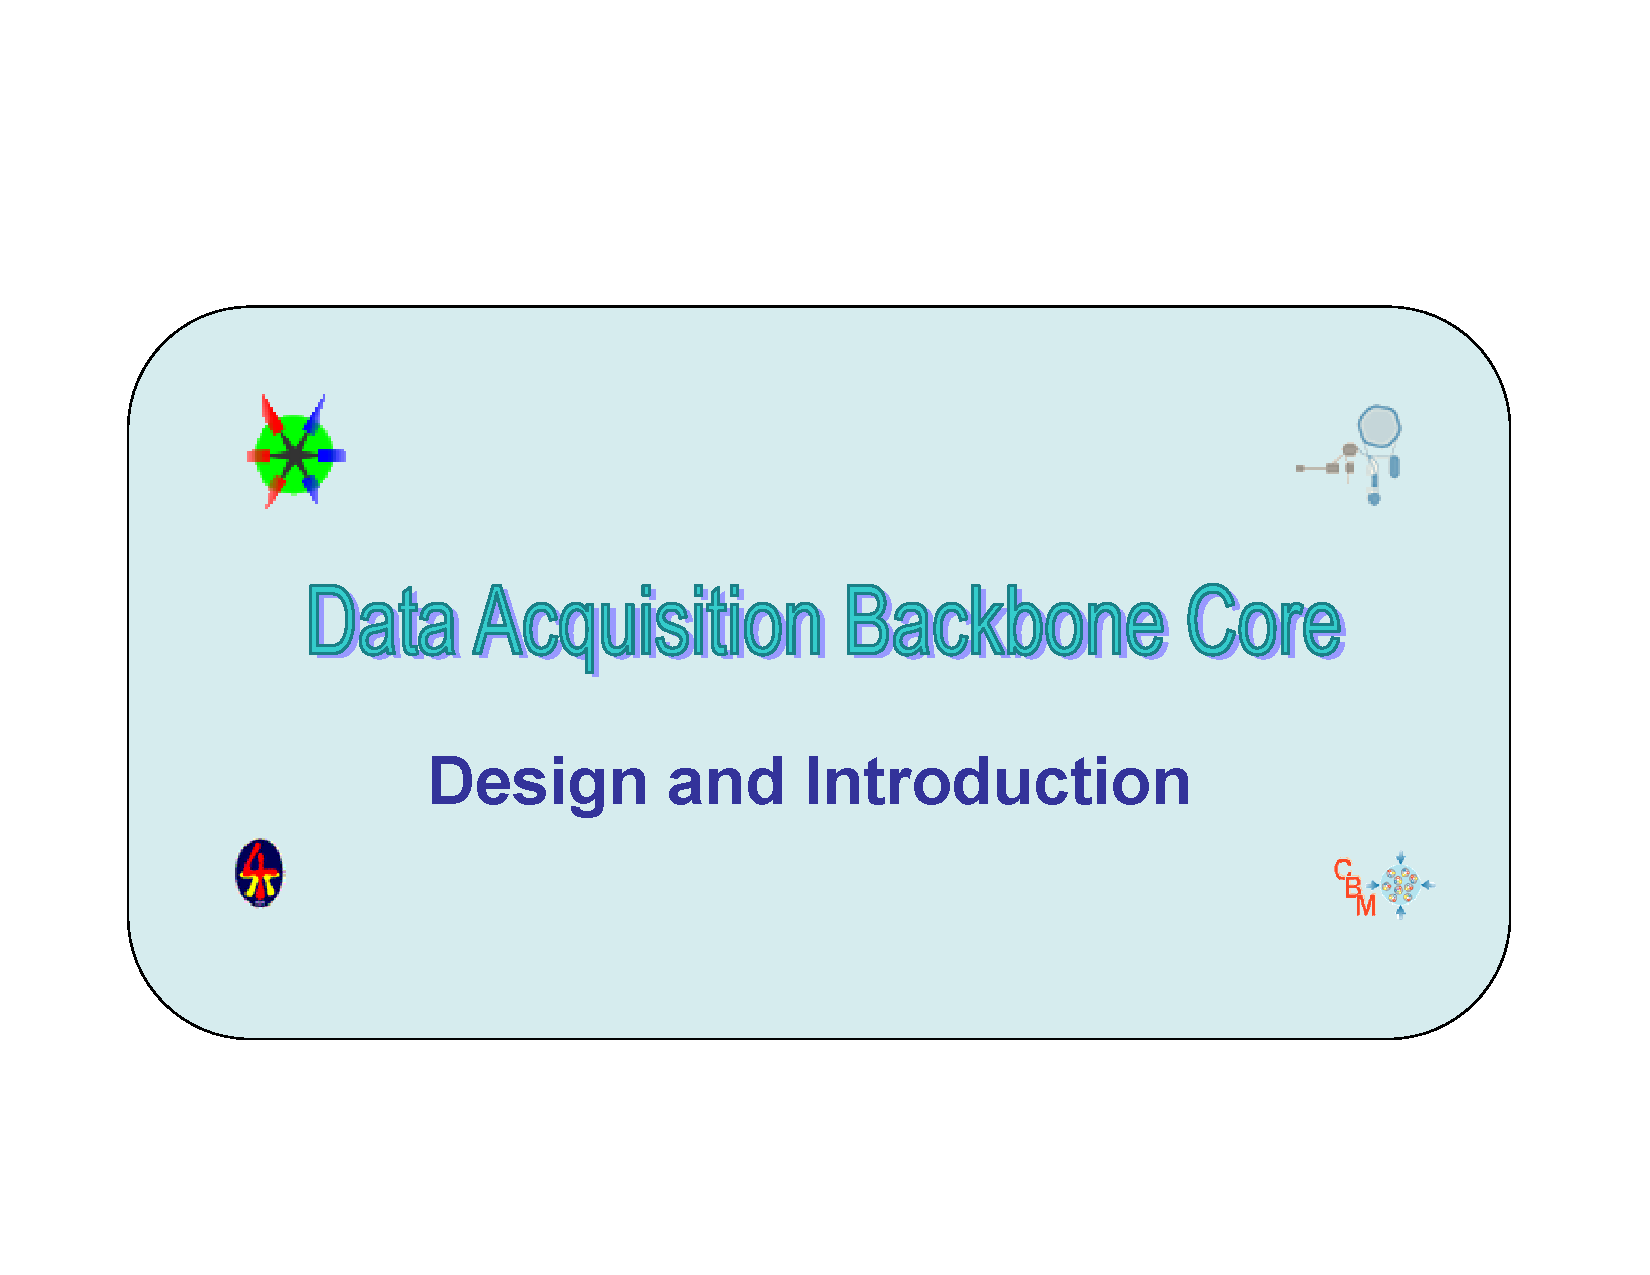
\includegraphics[width=.8\textwidth]
{frontpage}
\end{figure}
\vspace*{6cm}

\input{demo-docrev}
\vfill

\begin{center}
{\large March 2006} \\\vspace{0.5cm} {\large GSI Darmstadt}
\end{center}
 \cleardoublepage
%-----------------------------------------------------------------------------------
\thispagestyle{empty} \tableofcontents \thispagestyle{empty} \cleardoublepage
\pagenumbering{arabic}

\Chapter{Editorial}
[environment/dabc-editorial.tex]

\section{Structure of document}
The document is structured hierarchically. To make sure that files
to be included by \verb+\+input\{filename\} or \verb+\+include\{filename\}
can be located, set the following environment variables:\\
Linux:\\
export TEXINPUTS=\verb+<+topdirectory\verb+>+//:\\
Windows: If one uses fpTeX with WInEdt:\\
Append ;P:\verb+\+Application\verb+\+TeXLive2005\verb+\+bin\verb+\+win32 to PATH.\\
Set TEXINPUTS to x:\verb+\+topdirectory\verb+\+//;\\
(Systemsteuerung->System:Erweitert:Umgebungsvariablen)

The full document is built by command (we are on topdirectory):
\begin{verbatim}
pdflatex main-all
makeindex main-all.idx
pdflatex main-all
\end{verbatim}
or by {\tt make}. It builds the document in parts from the steering files in the directories.
On each subdirectory xxx there might be a main file main-xxx.tex to build a document 
from this directory only, i.e.
\begin{verbatim}
cd template
pdflatex main-template
makeindex main-template.idx
pdflatex main-template
\end{verbatim}
Alternatively on top directory the script 
\begin{verbatim}
makedoc <subdirectory>
\end{verbatim}
can be used. 
The files on directory {\tt template} can be used as templates, i.e. copied to a new subdirectory.
All occurences of XXX in file names and tex files should then be renamed properly.
The script {\tt rename.sh} can be used to do so:
\begin{verbatim}
. ../rename.sh XXX yyy
\end{verbatim}
replaces all {\tt XXX} to {\tt yyy} in tex file names and tex files.
(After that all eventually remaining {\tt *XXX*} files can be deletetd).\\
The file {\tt XXX-section.tex} contains commonly used tex commands.
It could be used as cut\&paste source.\\
Figures (pdf) can be located in any subdirectories, typically {\tt figures}.\\

\clearpage
Description of the files:
\subsubsection{Topdirectory}
\begin{compactdesc}
\item[Makefile] make file.
\item[makedoc] script to make a subdirectory.
\item[main-all.tex] main file to be texed. Includes all steer files from subdirectories.
\item[bibitem.tex] references
\item[dabc-glossary.tex] glossary
\item[dabc-requirements.tex] brief and informal list of requirements
\item[dabcclass.cls] document description
\item[rename.sh] script to rename/replace strings in file names and content.
\end{compactdesc}
\subsubsection{Subdirectory {\tt environment}}
\begin{compactdesc}
\item[dabc-docrev.tex] document name and revision information
\item[dabc-defs.tex] central definitions (included by all main files)
\item[dabc-post.tex] reference and index chapters (included by all main files)
\item[dabc-frontpage.tex] first page of top document
\item[dabc-people.tex] list of people
\item[dabc-preface.tex] this text
\item[dabc-work.tex] working packages
\end{compactdesc}
\subsubsection{Subdirectory {\tt controls}}
Example of a manual part. 
\begin{compactdesc}
\item[ctrl-docrev.tex] document name and revision information.
Is included by {\tt main-all.tex} and {\tt main-controls.tex}.
\item[main-controls.tex] main file to be texed.
Includes {\tt steer-controls.tex} and {\tt ctrl-docrev.tex}. Adjust document information here.
\item[steer-controls.tex] includes everything needed from this directory.
Is included by {\tt main-all.tex} and {\tt main-controls.tex}. Controls chapters.
\item[ctrl-section.tex] is an example section file (several sections)
 as included in the steering file.
\end{compactdesc}
All other directories below topdirectory have the main, docrev and the steer file.
\section{Formatting shortcuts}
Some macros are defined in the style file {\tt dabcclass.cls}
\subsection{Font styles}
\begin{compactitem}[$\bullet$] 
\item macro {\tt $\backslash$verba\{Verbatim\}} , tt \verba{Verbatim}
\item macro {\tt $\backslash$decl\{Declaration\}} , tt \decl{Declaration}
\item macro {\tt $\backslash$class\{Class\}} , bf em \class{Class}
\item macro {\tt $\backslash$func\{Function\}} , sl \func{Function}
\item macro {\tt $\backslash$member\{Member\}} , sl \member{Member}
\item macro {\tt $\backslash$strong\{Strong\}} , bf \strong{Strong}
\item macro {\tt $\backslash$keyw\{Keyword\}} , sf \keyw{Keyword}
\item macro {\tt $\backslash$param\{Parameter\}} , sf \param{Parameter}
\item macro {\tt $\backslash$comm\{Command\}} , sf \comm{Command}
\end{compactitem}
Example text:\\
When we have a \class{MyNewClass} it might have some \func{Functions} and some \member{Members}.
It also might have some \keyw{Constants} and \decl{Declarations}.
Fixed terms should be in \verba{Typewriter}. Text to be highlighted: \strong{Note!}.
DIM parameter and commands as \param{DataRate} and \comm{setBufferSize}
\subsection{Lists}
b is for begin, e for end
\begin{verbatim}
 {\bbul} = {\begin{compactitem}[$\bullet$]}
 {\ebul} = {\end{compactitem}}
 {\bcir} = {\begin{compactitem}[$\circ$]}
 {\ecir} = {\end{compactitem}}
 {\btri} = {\begin{compactitem}[$\triangleright$]}
 {\etri} = {\end{compactitem}}
 {\bbox} = {\begin{compactitem}[$\Box$]}
 {\ebox} = {\end{compactitem}}
 {\bnum} = {\begin{compactenum}}
 {\enum} = {\end{compactenum}}
 {\bdes} = {\begin{compactdesc}}
 {\edes} = {\end{compactdesc}}
\end{verbatim}
\bbul
\item bbul - ebul
\ebul
\bcir
\item bcir - ecir
\ecir
\btri
\item btri - etri
\etri
\bbox
\item bbox - ebox
\ebox
\bnum
\item bnum - enum
\enum
\bdes
\item[item] bdes - edes
\edes
\section{Naming conventions}
 \cleardoublepage
\Chapter{Preface}
[environment/dabc-preface.tex]
This document describes the requirements, design, and implementation of the
general purpose data acquisition backbone core \dabc.
This system is a result of the discussions about DAQ concepts for CBM,
Panda, and FutureDAQ started in 2004.

\section{Structure of document}
The document is structured hierarchically. To make sure that files
to be included by \verb+\+input\{filename\} or \verb+\+include\{filename\}
can be located, set the following environment variables:\\
Linux:\\
export TEXINPUTS=\verb+<+topdirectory\verb+>+//:\\
Windows: If one uses fpTeX with WInEdt:\\
Append ;P:\verb+\+Application\verb+\+TeXLive2005\verb+\+bin\verb+\+win32 to PATH.\\
Set TEXINPUTS to x:\verb+\+topdirectory\verb+\+//;\\
(Systemsteuerung->System:Erweitert:Umgebungsvariablen)

The full document is built by command (we are on topdirectory):
\begin{verbatim}
pdflatex main-all
makeindex main-all.idx
pdflatex main-all
\end{verbatim}
or by {\tt make}. It builds the document in parts from the steering files in the directories.
On each subdirectory xxx there might be a main file main-xxx.tex to build a document 
from this directory only, i.e.
\begin{verbatim}
cd template
pdflatex main-template
makeindex main-template.idx
pdflatex main-template
\end{verbatim}
Alternatively on top directory the script 
\begin{verbatim}
makedoc <subdirectory>
\end{verbatim}
can be used. 
The files on directory {\tt template} can be used as templates, i.e. copied to a new subdirectory.
All occurences of XXX in file names and tex files should then be renamed properly.
The script {\tt rename.sh} can be used to do so:
\begin{verbatim}
. ../rename.sh XXX yyy
\end{verbatim}
replaces all {\tt XXX} to {\tt yyy} in tex file names and tex files.
(After that all eventually remaining {\tt *XXX*} files can be deletetd).\\
The file {\tt XXX-section.tex} contains commonly used tex commands.
It could be used as cut\&paste source.\\
Figures (pdf) can be located in any subdirectories, typically {\tt figures}.\\

\clearpage
Description of the files:
\subsubsection{Topdirectory}
\begin{compactdesc}
\item[Makefile] make file.
\item[makedoc] script to make a subdirectory.
\item[main-all.tex] main file to be texed. Includes all steer files from subdirectories.
\item[bibitem.tex] references
\item[dabc-glossary.tex] glossary
\item[dabc-requirements.tex] brief and informal list of requirements
\item[dabcclass.cls] document description
\item[rename.sh] script to rename/replace strings in file names and content.
\end{compactdesc}
\subsubsection{Subdirectory {\tt environment}}
\begin{compactdesc}
\item[dabc-docrev.tex] document name and revision information
\item[dabc-defs.tex] central definitions (included by all main files)
\item[dabc-post.tex] reference and index chapters (included by all main files)
\item[dabc-frontpage.tex] first page of top document
\item[dabc-people.tex] list of people
\item[dabc-preface.tex] this text
\item[dabc-work.tex] working packages
\end{compactdesc}
\subsubsection{Subdirectory {\tt controls}}
Example of a manual part. 
\begin{compactdesc}
\item[ctrl-docrev.tex] document name and revision information.
Is included by {\tt main-all.tex} and {\tt main-controls.tex}.
\item[main-controls.tex] main file to be texed.
Includes {\tt steer-controls.tex} and {\tt ctrl-docrev.tex}. Adjust document information here.
\item[steer-controls.tex] includes everything needed from this directory.
Is included by {\tt main-all.tex} and {\tt main-controls.tex}. Controls chapters.
\item[ctrl-section.tex] is an example section file (several sections)
 as included in the steering file.
\end{compactdesc}
All other directories below topdirectory have the main, docrev and the steer file.
\section{Naming conventions}
 \cleardoublepage
\Chapter{DABC team}

\begin{compactitem}[$\bullet$]
\item {\bf Darmstadt, Germany, GSI }
J.~Adamczewski,
E.~Badura,
H.~Deppe,
H.~Essel,
H.~Flemming,
B.~Kolb,
S.~Linev,
W.F.J.~M{\"u}ller

\item {\bf Heidelberg, Germany, Kirchhoff-Institut f{\"u}r Physik,
Universit{\"a}t Heidelberg\footnotemark[1] }
U.~Kebschull (Universit{\"a}t Leipzig),
I.~Kisel,
V.~Lindenstruth,
G.~Tr{\"o}ger

\item {\bf Mannheim, Germany, Inst. of Computer Engineering,
Universit{\"a}t Mannheim \footnotemark[1]}
U.~Br{\"u}ning,
A.~Kugel,
R.~M{\"a}nner,

\footnotetext[1]{membership to be confirmed}
\end{compactitem}

\vspace{10cm}


\noindent {\bf Acknowledgement}

\noindent We acknowledge the support of the European Community-Research Infrastructure Activity
under the FP6 "Structuring the European Research Area" programme
(HadronPhysics, contract number RII3-CT-2004-506078).
Besides GSI, universities of Heidelberg, Mannheim are participating.
 \cleardoublepage
\Chapter{Requirements pin board}
[dabc-requirements.tex]\\
This list is rather about reminders. As soon as the items are addressed somewhere else,
they can be eliminated here.
\begin{enumerate}
\item It must be possible to partition the DAQ by configuration.
\item System must run with or without trigger
\end{enumerate}
 \cleardoublepage
[environment/dabc-work.tex]
Definition of work packages
\section{Hardware}
\section{Software}
\subsection{Framework}
\subsubsection{GUI}
\section{Controls}
 \cleardoublepage

%------------------------------------------------------------------------------------
\setcounter{chapter}{0}
\chapter{Documents}
Document names: DABC-c, where c=component key. Date in form yyyy-mm-dd.
Revision in form v.sv.b.\\
\\Titel: DABC Introduction
\begin{table}[h]
\begin{tabular}{|p{2.8cm}|p{2.0cm}|p{3.0cm}|p{1.6cm}|p{5.0cm}|} \hline
Document   & Date        & Editor       & Revision & Comment \\
\hline DABC-intro & 2008-12-18 & Hans G.Essel & 1.0.0    & First
scetch \\ \hline
\end{tabular}
\end{table}

%\input{dtor/dtor-docrev}
\\Titel: DABC: User Manual
\begin{table}[h]
\begin{tabular}{|p{2.0cm}|p{1.9cm}|p{3.2cm}|p{1.5cm}|p{5.8cm}|} \hline
Document   & Date        & Editor       & Revision & Comment \\
\hline DABC-user & 2009-01-05 & Hans G.Essel & 1.0.0      &
First scetch \\ \hline
\end{tabular}
\end{table}

\\Titel: DABC: Programmer Manual
\begin{table}[h]
\begin{tabular}{|p{2.0cm}|p{1.9cm}|p{3.2cm}|p{1.5cm}|p{5.8cm}|} \hline
Document   & Date        & Editor       & Revision & Comment \\
\hline DABC-prog & 2009-01-04 & Hans G.Essel & 1.0.0      &
First scetch \\ 
\hline DABC-prog & 2009-03-10 & J�rn Adamczewski-Musch & 1.0.1      &
Second scetch \\ 
\hline
\end{tabular}
\end{table}

\\Titel: DABC: reference manual
\begin{table}[h]
\begin{tabular}{|p{2.8cm}|p{2.0cm}|p{3.0cm}|p{1.6cm}|p{5.0cm}|} \hline
Document   & Date        & Editor       & Revision & Comment \\
\hline DABC-ref & 2009-01-05 & Hans G.Essel & 1.0.0      &
First scetch \\ \hline
\end{tabular}
\end{table}

%\\Titel: FutureDAQ Demonstrator Software
\begin{table}[h]
\begin{tabular}{|p{2.8cm}|p{2.0cm}|p{3.0cm}|p{1.6cm}|p{5.0cm}|} \hline
Document   & Date        & Editor       & Revision & Comment \\
\hline DAS-D-SW-06 & 2006 Oct 20 & Hans G.Essel & 0.9-2    & First
scetch \\ \hline
\end{tabular}
\end{table}

%\\Titel: FutureDAQ Demonstrator Hardware
\begin{table}[h]
\begin{tabular}{|p{2.8cm}|p{2.0cm}|p{3.0cm}|p{1.6cm}|p{5.0cm}|} \hline
Document   & Date        & Editor       & Revision & Comment \\
\hline DAS-D-HW-06 & 2006 Mar 13 & Hans G.Essel & 0.9      & First
scetch \\ \hline
\end{tabular}
\end{table}

\input{controls/ctrl-docrev}
%\input{simulation/simu-docrev}
%\\Titel: FutureDAQ Demonstrator Testing
\begin{table}[h]
\begin{tabular}{|p{2.5cm}|p{2.0cm}|p{3.0cm}|p{1.6cm}|p{5.0cm}|} \hline
Document   & Date        & Autor       & Revision & Comment \\
\hline DAS-TEST-06 & 2006 Nov 1 & J.Adamczewski S.Linev & 0.9 &
Draft
\\ \hline
\end{tabular}
\end{table}

\cleardoublepage
%----------------------------------------------------------------------------------
%\chapter{Work packages}
%[environment/dabc-work.tex]
Definition of work packages
\section{Hardware}
\section{Software}
\subsection{Framework}
\subsubsection{GUI}
\section{Controls}
 \cleardoublepage
% The parts structure may be useful later
%------------------------------------------------------------------------------------
\part{Introduction and Overview}
% DABC: Introduction and Overview
% This file is included from top directory in dabc environment.
% enter all chapters of introduction here
\section{DAQ for CBM}

The communication and processing needed between the front-end electronics,
generating digitized detector information, and the archival storage, where
the complete context of selected candidate events is recorded, can be
structured and organized in several ways.
The solution described in \cite{CBM-stat-rep} is guided by two principles:
processing is done after event building and it is done in a
structured processor farm.
It is well adapted to the type of processing needed in the CBM experiment
and leads to a straightforward and modular architecture.

\begin{figure}[htb]
\centering\includegraphics[width=.8\textwidth]
{demof-daq-all}
\caption{CBM overall data processing architecture}
\label{fig:daq-all}
\end{figure}

A logical data flow diagram is shown in Fig.~\ref{fig:daq-all},
indicating the data sources and processing elements as boxes and every
form of interconnection networks as ovals.
\clearpage

\section{Demonstrator mission}
\index{Demonstrator!mission}
\hyperdef{in}{mission}{[Marker:in.mission]}\\
The final DAQ system will be quite complex and involves many
technologies which are at the limits of today possibilities.
Therefore it is necessary to start early with a system which can
be implemented in the next years without showing up the full final
performance needed. This system, a \DDA, is useful in four
respects.
\subsection{Demonstration of key technologies}
\index{Demonstrator!technology}
The first task is to prove the key technologies needed, maybe with
less performance.
\begin{compactitem}[$\bullet$]
\item FEE: self-triggered, data push, conditional RoI based readout
\item CNet: combined data, time, control, and RoI traffic
\item TNet: low jitter clock and synchronization over serial links
\item BNet: high bandwidth switched network for event building
\item ECS: integrated control system
\end{compactitem}
\subsection{Test bed for prototypes}
All components will need iterations. A testing environment is
needed from the beginning.
\begin{compactitem}[$\bullet$]
\item Hardware
\item Firmware
\item Controls
\item Software
\end{compactitem}
\subsection{Functional DAQ for detector tests}
There are many questions concerning detector performance.
Prototypes will be developed. They can only be tested with a DAQ
system with the same characteristics as the final one. The whole
readout chain must be available to prove that a triggerless
readout is feasible.
\subsection{General purpose DAQ for medium sized experiments}
To prove that a highly distributed system scales it is necessary
to install at least a medium sized setup. This can only be
afforded if it is used in production for an experiment.

\section{Demonstrator use cases}
\index{Demonstrator!use cases}
According the mission there are several use cases or scenarios:
\subsubsection{Frontend test bed}
The new components FEB, DCB, and ABB and their connections must be tested.
The timing system and the triggered/non-triggered mode must be tested.
\subsubsection{Detector test bed}
Detector tests with a free running system are needed to verify that the data rates
are not very much bigger that expected (dark noise).
\subsubsection{Switched event building}
Independent of the data sources (ABB or GEB) several mechanisms for the switched
event building must be implemented and tested.
\subsubsection{DAQ framework and control systems}
There are still several options for the choice of the control system.
\subsubsection{MBS replacement}
\index{Demonstrator!MBS}
Very probably there will be no complete replacement of the MBS possible for the next years.
One could envision that the MBS frontend nodes, i.e. the readout nodes
send their subevent data peer to peer to new event builder nodes (new MBS mode).
\subsubsection{Hybrid setup}
If the system should run in production, very probably a hybrid of MBS for ancillary components
and new frontends will be needed.

\section{Demonstrator architecture}
As a first step the \DDA~ shall be used to investigate practically the technologies needed.

\begin{figure}[htb]
\centering\includegraphics[width=.8\textwidth]
{demof-all}
\caption{\DDA~ overall data processing architecture}
\label{fig:daq-over}
\end{figure}

The system can be described in several dimensions:
\begin{compactdesc}
\item[Hardware] There are mainly three boards with different tasks but similar architecture.
\item[Data formats] The data and time stamp formats must be defined early because they are
interpreted at many occasions. A change would have big impact.
\item[Data flow models] Mechanisms how the data is moving throughout the system.
\item[Software framework] What frameworks are used. We should not start from scratch.
\item[High level software] Runs wherever Linux is running.
\item[Board level software] Mainly the FPGA codes
\item[Controls] Several sorts of controls
\end{compactdesc}

\subsection{Hardware}
The hardware components as shown in Fig.~\ref{fig:daq-over} are
summarized with their key features.
\subsubsection{Front End Electronics board FEE}
General purpose chamber-mountable board with ADCs (4*4 channels,
65 MHz sampling, 10-12 bit), FPGA (Virtex-4, PPC, Ethernet MAC,
MGT plus SDRAM, CPLD, NVRAM), plugable to preamp/chapers. A
version utilizing pipeline TDCs (ns resolution) possible. Two
clock domains: receive clock of 312.5 MHz (timing and trigger) and
sampling clock with 62.5 MHz (measurement). Four pair of LVDS
bi-directional links (625 Mbps).
\subsubsection{Data Combiner board DCB}
Four bi-directional LVDS links to FEB, Ethernet, MGT with SFP
optical link to ABB, same FPGA. A test layout of such board is shown in Fig.~\ref{fig:dcb}.
A possible connection to the between FEE and DCB boards is shown if Fig.~\ref{fig:fee-dcb}
\subsubsection{Active Buffer board ABB}
PCIe board, 4 - 8 MGT/SFP optical links to DCBs, same FPGA.
\subsubsection{Timing board}
Similar to DCB, gets optional trigger inputs, generates clock and distributes through
optical splitters to DCBs.
\subsubsection{Event builder}
Standard PC with GE, InifiniBand switch.


\subsection{Data formats}
See also \hyperref{http://www-linux.gsi.de/~mbs/main-software.pdf}{sw}{data}{Software paper}.
\subsubsection{Raw data stream}
The data must be formatted on the FEE boards to achieve the following requirements:
\begin{compactenum}
\item compressed
\item coded geographical address
\item incremental time stamps
\item time epoch markers
\end{compactenum}
The event building is done through a switched network.
Logical entities to be switched are epochs.
Data before switching may be stored/retrieved in a binary format for testing and/or
development..
It should be foreseen that data has to be reformatted before the switching, because different
subsystems might produce different data formats. Eventually the time sorting might be done.
After the switching, the event definition has to be done.
At that point all data must be repacked.
\subsubsection{Event definition data}
This intermediate format is a full time ordered compressed data stream of an epoch.
Optionally it may contain multiplicity histograms to accelerate later event definition.
Data may be stored/retrieved in this format.
\subsubsection{Event format}
After event definition events must be formatted and stored.

\subsection{Software}
\subsubsection{Board level software}
Software running on the FPGAs. The data flow from the FEE through
the DCB to the ABB is controlled by FPGAs.
\subsubsection{Data mover}
The data dispatchers (task on standard PCs with Linux) read the
data stream via PCIe from the ABB boards and send it via a fast
network (GE or IB) switch to the event builder tasks (same PCs)
using the links bi-directional.
\subsubsection{Data processing}
From the event builder task the formatted events are handed over
to data processing tasks for event filtering and archiving. These
tasks can run optionally on separate machines.
\subsection{Controls}
For the three main fields of detector controls, DAQ controls, and board controls
there are currently three products under test:
\begin{compactdesc}
\item[EPICS] Well known control system, widely used in accelarator and classical controls.
SNMP interface is available for monitoring clusters and net devices.
\item[LabView] Standard slow control at GSI.
\item[SysMES] Configuration control system developed at KIP. Has CA interface to work with
EPICS and SNMP.
\item[xDAQ] DAQ framework of CMS
\end{compactdesc}
Because it might be not possible to make a decision for one of these to be used exclusively
one should investigate/implement interoperability.
Communication standards in question:
\begin{compactitem}
\item DIM: DIM server in an EPICS IOC as first test bridge
\item CA: LabView CA client available
\item SOAP: provided by xDAQ, Java interface available.
\item CA: EPICS IOC (xDAQ application) gateway to xDAQ infospace
\end{compactitem}
The DAQ controls must provide the following functionality:
\begin{compactitem}
\item Control tasks on remote machines
\item Communicate with all tasks
\item Mechanism to store/retrieve the whole setup
\item Monitor setup, status, data flow, and performance
\item Control data flows
\item Visualization and GUI
\end{compactitem}
 \cleardoublepage
[introduction/in-dabc-concept.tex]
\section{Concept}
% define a marker to be referenced from outside:
\hyperdef{dabc}{concept}{[Marker:dabc.concept]}\\
As mentioned in the introduction, there are several scenarios or
use cases for the \DDA~ reflecting differing requirements and
delivery dates.
\subsection{\DDA~ use cases}
\index{Demonstrator!use cases}
\subsubsection{Detector test bed}
Detector tests with a free running system are needed to verify
that the data rates are not very much bigger than expected (dark
noise).
\subsubsection{Switched event building}
Independent of the data sources (\ABB~ or GigabitEthernet) several mechanisms for the switched
event building must be implemented and tested.
\subsubsection{DAQ framework and control systems}
There are still several options for the choice of the control system. The \xdaq~ framework
provides several communication mechanisms. The control system not necessarily must be \xdaq~ but
could be e.g. EPICS based. In such a case gateways must be implemented.
\subsubsection{\mbs~ replacement}
\index{Demonstrator!MBS} Very probably there will be no complete
replacement of the \mbs~ possible for the next years. A very big
amount of existing hardware of running \mbs~ systems cannot be
replaced neither they can be attached directly to the new DAQ
framework. At least the effort to replace the software running on
the front-end CPUs (RIO, Lynx, \mbs~) would be too big, if
possible. Instead one could envision that the \mbs~ front-end
nodes, i.e. the readout nodes, send their sub-event data peer to
peer to new event builder nodes (new \mbs~ mode). Each of these
nodes functions as sub-event receiver (Ethernet, TCP) and sends
the data for event building through the data transport network
like InfiniBand to the others and functions also as event
processor. The Ethernet input channel replaces the \ABB~input
channel.
\subsubsection{Hybrid setup}
If the system should run in production, very probably a hybrid of
\mbs~ for ancillary components and new front ends will be needed.
When running in triggered mode, the trigger of the new components
must be synchronized with the \mbs~ trigger system. In triggerless
mode the \mbs~ data must be time stamped or \mbs~ triggers must be
injected and recorded in one of the time stamped data streams by
connecting the trigger bus directly to an \FEB.
\subsubsection{Front end test bed}
The new components \FEB, \DCB, and \ABB~and their connections must be tested.
The timing system and the triggered/non-triggered mode must be tested.

\subsection{The name}
Because the systems described might be also used by other
experiments it might evolve to more than a dabcnstrator. At the
other hand it will not provide components of the front-end side
but rather provide the hooks and plug-ins to attach a big variety
of front-end systems and components. There is one principal
restriction, however, in the current design. There is nothing like
a 2nd level trigger. That means, that we assume that the full data
rate can be switched through a network for event building.
However, a congestion prevention must be provided generating dead
time for the detector readout. From this point on we have only
event filters. The front-ends might however be triggered or free
running.

The dabcnstrator as a production system would be rather a backbone. Therefore we propose a name like\\
Data Acquisition Backbone Framework {\bf DBF} (DataBaseFormat!) or {\bf ABF}\\
Data Acquisition Backbone System {\bf DBS} (Deutscher Bildungs-Server) or {\bf ABS}\\
Data Acquisition Backbone Core {\bf DABC} or {\bf ABC}\\
FAIR Acquisition Backbone {\bf FAB}

\section{\dabc~ architecture}
\begin{figure}[htb]
\centering\includegraphics[width=.8\textwidth] {dabc_sw-over_4}
\caption{\dabc~ data flow and components}
\label{fig:dabc_sw-over_4}
\end{figure}

\section{Implementation phases}
One can identify four implementation phases, i.e. time scales:
\begin{compactenum}
\item \mbs~ front end support
\item Hardware tests and basic functionality of framework
\item Detector test
\item Production system
\end{compactenum}
Phase 0 might be in the beginning necessary for elementary test of the boards and the data links.
The software of phase 0 will be "experimental" and not part of the system.
\section{Requirements}
\subsection{Frontend test bed}
Phase 0, 1
\begin{figure}[htb]
\centering\includegraphics[width=.8\textwidth] {dabcf-all}
\caption{\dabc~ overall data processing architecture}
\label{fig:dabc-daq-over}
\end{figure}

\begin{figure}[htb]
\centering\includegraphics[width=.8\textwidth]{sw-over} % pdf file
\caption{Overall data streams architecture}
\label{fig:dabc-struct-over} % give it a name for references
\end{figure}

Fig.~\ref{fig:dabc-daq-over} shows the hardware components,
fig.~\ref{fig:dabc-struct-over} shows the data streams.
\subsection{Detector test bed}
Phase 2
\subsection{Switched event building}
Phase 2
\subsection{DAQ framework and control systems}
Phase 2
\subsection{\mbs~ front-end support}
Phase 1
\subsection{Hybrid setup}
Phase 4
\section{DABC framework requirements}

S.Linev, 23.01.2007

This is short description of required functionality, possible use cases and implementation details for some basic components of DABC framework.

\subsection{Basic overview}
I propose to build our framework as data flow model, where two main types of entities are exists: data processing units (modules) and communication (transport) layer between modules. This kind of approach used in SystemC and many ideas from this framework can be used.

\subsubsection{Transport layer}
This is major component of complete framework. Its main aim is the transport of basic data types (integer, floats) and arbitrary data packets between different parts of the distributed system. Transport can be local (inside one application) or global. Transport can be pear-to-pear or network-kind, when in addition destination address is specified. 
Interface from program code to transport should be done via 'port' entity, which should not depend from specific transport implementation. In normal operations mode user uses only port functionality to send/receive data. 
Ports are connected with each other during initialization phase. At this phase configured implementation of transport should be created and assigned for this port. 
By default, all ports are bidirectional, but one should be able to restrict port only for input or only for output. Each port can have name and, if required, data type identifier (string or number id). 
Transport layer approach gives flexibility to exchange different transports without exchange of data processing code.
Another advantage of intermediate transport layer between modules is possibility to store flowing data into the file. Later this data can be used for debugging of parts of the complete system instead of real data one can provide data from log file(s). 

\subsubsection{Processor unit (module)}
This is place for program code. All data manipulation should happen only inside modules. Communication with other modules should only be done via ports. In module constructor required number of ports should be created and registered to the module. Module should have functionality to list all ports afterwards. 

\subsubsection{Connection configuration approach}
First of all, application should be able to browse/search full hierarchy of the modules. As a result, one will have access to all ports, parameters, control values, which are available via module interface. During application startup modules should be created and local (application-wide) interconnection should be established. Connection with external nodes (or other application from the same node) can be configured locally or via control interface from operator node. 
This is static connection approach, while connections should be established before module can start working. But such approach may fail when network has dynamic nature, i.e. number of nodes or number of running processes increases/decreases during system run. Then system should be able dynamically establish new connection or brake existing ones. One possible solution is dynamic connection management, where modules could requests necessary connection to external module. For such functionality complete hierarchy of nodes/applications/processes/modules should have unique identifiers. One should avoid situations that module itself decides which transport used for connection. Connection manager should itself create appropriate transport and establish connections. 

\subsubsection{Buffer management}
As long as generic transport should support zero-copy data transfer, one should have application-wide buffer management, which takes care about buffers allocation/holding/release action. 

\subsection{Use cases}
1. Generic DAQ with several modules, connected via transport layer. One can imagine situation, when all modules run on single node, but one may also require to reconfigure same DAQ to run on several nodes. \\
2. Specific B-Net implementation. In this case one cannot use standard interface. Most probably, one should directly access transport from module to explore all functionality of specific network (for instance, MPI or verbs).

\subsection{Implementation details}
Communication port 
Here one supposes to have one common class (TTransport), which deliver interface, used by TPort class to send/receive data. TPort should not have any transport-specific code. 
Important question is usage of templates. SystemC port class is defined as template, where transferred data type is template parameter. This allows arbitrary port kinds, but complicates implementation for us, especially when one needs to communicate with different nodes and OS. I propose to support only following types: arbitrary binary buffer, integer (int64t), 64-bit double, null-terminated string. As result, one should implement four TPort::Send() methods, each for mentioned data types. In port constructor user should clearly specify which type will be used. 
Type identifier can be integer or string. Some types, deriver from binary buffer, can has it own types identifier. For instance, output port of event builder, can be identified as 'DABCFullEvent'. Probably, one can use here name, derived from data-format plugin, for instance 'MBS10\_1Event'. 
While port will have type identifier parameter, one can provide type-safety check during modules connection. Generally, types of connected port should match with each other. One also can detect error situations like two output ports are connected or similar.
Each port should have configurable size input and output queues. In the queue one store send/received values. For binary data buffer identifier is saved. 
Very important question: how we notify module when data is arrived (send). First, one should be able to use polling approach. For that appropriate flag should be defined in TPort class. One should be able to use queue size for this purpose. Second, kind of TPort::Wait() method should be implemented. It suspends receiver thread until new data is arrived. When it happens, data should be placed in receiving queue as well. Third, one can support call-back function, which is called when new data is arrived. In call-back function, defined in module class, one can immediately process incoming data. 
Seems to be, call-back approach cannot be combined with first two (wait or pool) for single port, therefore one should clearly specify port notification type at the time when port is created. One should also investigate, if notification required for the output port. 

\subsection{Transport}
Specific kind of transports (dapl, socket, pipe) should be implemented, as TTransport subclasses. Interface of TTransport class should be suited both for pear-to-pear and network-kind transport. For instance, TTransport::Send() method can have two arguments, where first is data to transfer (buffer reference or integer or float or string) and second argument is destination address (by default, -1 and ignored by peer-to-peer transport). \\
For the local (inside application) communication one need implementation which is able to transfer data between two threads. Actually, it can be single object which is associated with both input and output ports. Only buffer reference (buffer id) will be moved. Buffer itself will remain busy until receiver releases it. Actually, one can imagine situation, when several modules running in single thread and should communicate with each other. In this case call-back function approach can be most optimal (no need for additional communication threads at all).
For the global (inter-node or inter-application) communications one need of course separate objects on receiver and sender sizes. In that case transport object is responsible for release/lock of the buffers. 

\subsection{Module}
Module is aggregation of input/output ports and methods to transform data from inputs to outputs. Module should keep (be able to reproduce) list of all available ports.
Combination of several modules can be combined in one valid super-module. From outside it should be seen as normal module with several ports, inherited from sub-modules.
Probably, module should have separate list of parameters, which can be changed/viewed from outside by controlling system. 

\subsection{Buffers management}
It should be application-wide manager for buffers, allocated for data transport or just for application use. 
Because of this reason one can add some methods to TPort class, which allocates required number and size of buffers, which are suitable for transport, used for port connection. 
Buffers in manager should be grouped in subsets. Inside subset all buffers can (have to?) have same size. Buffer id (64 bit) can be combined from subset-id (16 bit) and buffer number (48 bit). 
Subset approach allows us to create one object per subset (like TBuffersSubset), not one object per buffer. This is very useful in the case, when many small buffers should be allocated. This also can be used in dapl/verbs transport implementation. There one should only register complete subset memory region and not separate memory buffers.
Actually, TBuffersSubset also can consist of set of normal buffers, where one object correspond to one buffer. 
For each buffer in subset one should keep additional information. It should be at least boolean flag, which indicate if buffer in use. One can also allow additional buffer information like data format type, individual buffer size, buffer shift and so on for each separate buffer in subset.

\subsection{Generic question} 
Which OS should be supported? Only Linux or any Unix-like? LynxOS support? 
Windows support: CYGWIN or native Win32/Win64 API or not supported at all? Probably, one can support some basic module functionality plus threading plus socket connection to enable some end-user activity on Windows. An be recognized, as low-priority task.
Do we using only glibc and pthread, or some additional library? Other thread implementations?
How we use templates? Most concern can be about list of objects like list of ports, list of parameters and so on. If we do not use template, ROOT-like approach with TNamed and TList classes should be use. This is not type-safe, but simplify search by name or similar functionality. In case of templates search methods should be implemented each time.
Do we use some basic class like TObject at all? Probably, yes. It can be useful not only in lists, but also to introduce hierarchy via parent-child relationship between objects. This provide us unique naming scheme for all objects in the system. Another solution for hierarchy: object manager, where any object property (name, config parameters and so on) stored independent from object itself.

\subsection{Requirements}
Lets summarize requirements for different components of the framework.
\subsubsection{Port}
\begin{compactitem}[$\bullet$]
\item communication entity for sending/receiving data from/to user code;
\item single TPort class, independent from specific transport implementation;
\item bi-directional or only input or only output (configurable on creation time)
\item supported data format: binary buffer, null-terminated string, integer, floats (configurable on creation time);
\item safety checks during connection: type safety, in/out comparison;
\item notification via wait/poll mechanism or via call-back (configurable on creation time);
\end{compactitem}
\subsubsection{Transport}
\begin{compactitem}[$\bullet$]
\item bidirectional data transfer between modules ports;
\item same basic TTransport class for all implementation;
\item both peer-to-peer and network in one interface;
\item local transport between modules in two threads;
\item local transport between modules in single thread;
\item global transport via pipe, socket, dapl, mpi, verbs, XDAQ peer-to-peer;
\item logging of data flow. 
\end{compactitem}
\subsubsection{Module}
\begin{compactitem}[$\bullet$]
\item keep list of ports;
\item keep list of parameters;
\item can be triggered by timer;
\item debugging possibility with use of log data;
\item unique identifier (name) over all system.
\end{compactitem}
\subsubsection{Buffer management}
\begin{compactitem}[$\bullet$]
\item buffer managed by subsets of the same size and kind of buffers;
\item TBufferSubset can has special implementation for specific transports (like verbs, dapl);
\item TPort should has methods to allocate appropriate subsets in manager;
\end{compactitem}
\subsubsection{Generic}
\begin{compactitem}[$\bullet$]
\item use of exception for error handling;
\item full support of Linux, LynxOS;
\item partial support of Windows;
\item no templates in basic transport functionality;
\item objects hierarchy via object manager or parent-child relationship;
\item basic TObject class, TList, TObjArray classes.
\end{compactitem}

 \cleardoublepage
[introduction/in-dabc-design.tex]
\section{Design}
\subsection{Task layout}
\begin{figure}[htb]
\centering\includegraphics[width=.8\textwidth] {dabc_sw-over_3}
\caption{\xdaq~ entities} \label{fig:dabc_sw-over_3}
\end{figure}
Figure \ref{fig:dabc_sw-over_3} shows the task layout of \xdaq~.
On each node there is at least one executive which controls
the \xdaq~ applications. The applications run in threads
thus being scheduled and sharing memory. Applications also may start and
control threads (work loops).\\
The executive also is the communication stub through the Web interface or the
DIM gateway. The executive addressspace is the scope of the infospace. The
infospace provides mechanisms to access parameters across applications
and subscribe for parameter changes. The DIM gateway subscribes for
parameters in the infospace and serves them to DIM clients.\\
Figure \ref{fig:dabc_sw-over_4}, page \pageref{fig:dabc_sw-over_4} shows the data flow. 
There are two main
\xdaq~ executives. One runs the applications for the data input from the
front-end systems, the event building scheduler and the network senders.
The second one runs the event receiver applications for event tagging,
event building and event senders.
\clearpage
\subsection{MBS data input}
A \dabc~ input channel can connect to an \mbs~ transport and read LMD buffers.
The \mbs~ runs in a special \dabc-mode without event spanning over buffers.
Because buffers now can have any size, one buffer per stream can be configured
to avoid event spanning.

\subsubsection{Communication protocol}
\begin{compactenum}
\item The \dabc~ input channel connects to the \mbs~ transport.
\item An acknowledge message of 4 longwords is returned (endian=1, size, buffers, streams).
For transport that means that \dabc~ needs a buffer of size x buffers bytes to store all
events of a stream completely (no fragments).
\item Start reading buffers. When the reading is slower than the \mbs~ can send,
the \mbs~ blocks!\\
\mbs~ transport sends buffers.
\item Close connection.
\end{compactenum}


\subsubsection{MBS control}
The remote \mbs~ system can be controlled completely by \dabc.
\mbs~ runs now DIM servers for monitoring and controls.
The \mbs~ is started by remote shell commands and controlled by
sending commands to DIM server. The controlling process as a DIM client
registers the \mbs~ status information for monitoring.
 \cleardoublepage
 \cleardoublepage
%-----------------------------------------------------------------------------------
\part{User Manual}
% DABC User Manual: Overview

% This file is included from top directory in dabc environment.
% enter all chapters of introduction here
\chapter{\dabc~ User Manual: Overview}
[user/user-overview.tex]
\lsection[Outline of this manual]{user-overview-outline}{Outline of this manual}
This \dabc\ User Manual contains all information that is necessary to
install and use the \dabc\ framework.

Chapter \paref{user-introduction} should be useful to understand the
most commonly used terms of \dabc.

Chapter \paref{user-setup-chapter} describes how to install the
\dabc\ packages on any linux machine, and how to set up the working
environment. Additionally, some typical use cases and their configuration
files are shown. 
The following chapters then give more detailed explanations how to operate
in different modes with the \dabc\ Java GUI:

Chapter \paref{user-gui-chapter}
covers the general functionality of the GUI
which is common for most applications. Especially, this 
is mostly sufficient
to control a DAQ cluster purely with one or several \dabc\ nodes.

Chapter \paref{user-gui-mbs-chapter} describes the \dabc\ GUI 
in a mode to control a pure \mbs data acquisition system without 
a native \dabc\ node.

The application use case for a mixed DAQ cluster, both with \dabc\ and \mbs\ nodes, is
treated in Chapter \paref{user-app-mbs-chapter}.

Chapter \paref{user-app-bnet-chapter} describes the use case of
a \dabc\ builder network (BNET), both with and without using \mbs\ .

Finally, Chapter \paref{user-app-roc-chapter} describes the use case of
ROC front-ends.

However, the scope of the \dabc\ User Manual does not contain 
detailed descriptions of the \dabc\ framework architecture, 
the software mechanisms, and the example programs. 
These subjects are treated thouroughly
in the \dabc\ Programmer Manual.

\lsection[Release Notes]{user-overview-release}{Release Notes}

\subsection{Version 1.0.01 (10. March 2009)} 
\bnum
\item Add IP multicast support in SocketTransport.
\item Add IB multicast support in verbs::Transport.
\item Possibility to add user-defined parameters directly in xml file - 
      in Context/User section.
\item If Context/Run/copycfg = true, config file will be copied to working
      directory of specified node, useful for cluster without common file system.
\item Implement all-to-all and multicast tests in net-test application.
\item Bugfix several minor errors in Verbs plugin.
\item Bugfix: suppress output of scripts running from ssh (caused problems with GUI).
\item Bugfix: GUI: Register DIM service after full instantiation of parameter object.
\item Bugfix: GUI: Histogram drawer had uninitialized field.
\enum

\subsection{Version 1.0.00 (26. February 2009)}
These are the features of the first official release:
\bnum
\item A Data Acquisition framework in C++ language for linux platforms
   with modular components for dataflow on multiple nodes.
   
\item Runtime environment with basic services for:
   threads, event handling, memory management, command execution, 
   configuration, logging, error handling

\item Plug-in mechanism for user defined DAQ applications

\item Plug-in mechanism for a control system. Features a finite state machine
   logic and parameters for monitoring and  configuration.
   The default implementation is based
   on the DIM protocol (http://dim.web.cern.ch/dim)

\item Java GUI to operate the standard DIM control system of \dabc/\mbs. 
   Fully generic evaluating \dabc\ process variables, but extendable
   by user written components.

\item Contains a sub-framework to set-up distributed event builder networks (BNET) 
 
\item Supports TCP/IP and InfiniBand/verbs networks for data transport

\item Supports formats and readout of GSI's standard DAQ system \mbs\
   (Multi Branch System). May also write data into \mbs\ listmode format,
   and may emulate MBS socket data servers.
   Additionally, MBS systems can be controlled by the DABC GUI.  
\enum

% 
% More specific functionality is described in the sections of the applications
% (as far as delivered with \dabc).
% 
% As examples we take sometimes the \dabc\ simulator plug-in which runs out of the box.
% 
% External application specific GUI add-ons cannot be described here.

 \cleardoublepage
\chapter{\dabc~ User Manual: Plugins}
[user/user-plugin.tex]
\section{\dabc plug-in mechanism }
 \cleardoublepage
\chapter{\dabc~ User Manual: Parameter}
[user/user-parameter.tex]
\section{\dabc~ parameters}
 \cleardoublepage
\chapter{\dabc~ User Manual: Commands}
[user/user-command.tex]
\section{\dabc commands}
 \cleardoublepage
\chapter{\dabc~ User Manual: Setup}
[user/user-setup.tex]
\lsection[Installing DABC]{user-install}{Installing \dabc}
\index{DABC!Installation}
When working at the gsi linux cluster, the \dabc~ framework is already installed and will
be maintained by people of the gsi EE department. Here \dabc~ needs just to be
activated from any gsi shell by typing {\tt . dabclogin}. In this case, 
please skip this installation section and proceed with following section \ref{user-env} describing
the set-up of the user environment.

However, if working on a separate DAQ cluster outside gsi, 
it is mandatory to install the \dabc~ software
from scratch. 
Hence the \dabc~ distribution is available for download at \hyperref{http://dabc.gsi.de}{}{}{http://dabc.gsi.de}.
It is provided as a compressed tarball of sources {\tt dabc1.tar.gz}.
The following steps describe the recommended installation procedure:

\bnum
\item {\bf Unpack this \dabc~ distribution} at an appropriate installation directory,
e.~g.~:
\begin{verbatim}
cd /opt/dabc; 
tar zxvf dabc1.tar.gz
\end{verbatim}
This will extract the archive into a subdirectory which is labelled
with the current version number like {\tt /opt/dabc/dabc\_1\_0.00}.
This becomes the future \dabc~ system directory.

\item {\bf Prepare the \dabc~ environment login script}:
A template for this script can be found at {\tt scripts/dabclogin.sh}
\bbul
  \item Edit the {\tt DABCSYS} environment according to your local installation directory. 
  This is done in the following lines:
  \begin{verbatim}
  export DABCSYS=/opt/dabc\_installations/dabc_1_0.00  
  \end{verbatim}  
  
  \item Edit the {\tt DIM\_DNS\_NODE} environment according to the machine where 
  the DIM name server \cite{DIM} for the \dabc~ control system will run:
   \begin{verbatim}
  export DIM_DNS_NODE=hostname.domain.de
  \end{verbatim}  
  \item Copy the script to a location in your global {\tt \$PATH} for later login,
  e.~g.~ {\tt /usr/bin}. Alternatively, you
  may set an \func{alias} to the full pathname of {\tt dabclogin.sh} in your shell profile.
\ebul

\item Execute the just modified login script in your shell to set the environment:  
  \begin{verbatim}
  . dabclogin.sh
  \end{verbatim} 
  This will set the environment for the compilation.

\item Change to the \dabc~ installation directory and start the build:
  \begin{verbatim}
  cd \$DABCSYS
  make
  \end{verbatim} 
  This will compile the \dabc~ framework and install a suitable version of DIM in a
  subdirectory of {\tt \$DABCSYS/dim}.

\enum

After succesful compilation, the \dabc~ framework installation is complete
and can be used from any shell after invoking {\tt . dabclogin.sh}
The next sections \ref{user-env} and \ref{user-setup} will describe further steps 
to set-up the \dabc~ working environment for each user.


\lsection[Set-up the DABC environment]{user-env}{Set-up the  \dabc~ environment}
\index{DABC!Environment set-up}
Once the general \dabc~ framework is installed on a system, still each user
must "activate" the environment and do further preparations to work with it.

\bnum
\item Execute the \dabc~ login script in a linux shell to set the environment.
At gsi linux installation, this is done by  
\begin{verbatim}
  . dabclogin
  \end{verbatim} 
For the user installation as described in above section \ref{user-install},
by default the script is named   
  \begin{verbatim}
  . dabclogin.sh
  \end{verbatim} 
The login script will already enable the \dabc~ framework for
compilation of user written components. Additionally, 
the general executable {\tt dabc\_run} now provides
the \dabc~ runtime environment and may be started directly 
for simple "batch mode" applications on a single node. 

However, further preparations are necessary if \dabc~ shall be used with
DIM control system and GUI.

\item Open a dedicated shell on the machine that shall provide the DIM name server,
e.~g.~ {\tt ssh nsnode.cluster.domain}
Then call 
\begin{verbatim}
. dabclogin.sh
dimDns  
\end{verbatim} 
to launch the DIM name server. This is done \strong{once} at the beginning of
the DAQ setup; usually the DIM name server needs not to be shut down 
when \dabc~ applications terminate.

\item Set the DIM name server environment variable in any \dabc~ working shell (e.~g.~
the shell that will start the dabc gui later):
\begin{verbatim}
. dabclogin.sh
export DIM\_DNS\_NODE=nsnode.cluster.domain
\end{verbatim} 
Note that a user installation of \dabc~ framework may set this 
environment variable already in the general {\tt dabclogin.sh} script, if the DIM name server will 
mostly run for all users on the same default node (see section \ref{user-install}).  

\item Now the \dabc~ GUI can be started in such prepared shell by typing {\tt dabc}, (or 
{\tt mbs} for a plain \mbs~ gui, resp.). See below in gui section.  

\enum


\lsection[Setting up DABC user workspace]{user-setup}{Setting up \dabc\ user workspace}
\index{TODO!Setup}
To operate a \dabc\ application one should create a dedicated 
working directory to keep all relevant files:
\bbul
\item Setup files for \dabc\ (XML).
\item Log files (text).
\ebul
The GUI may run on a different directory with no access to the \dabc\ working directory.
There we place:
\bbul
\item Data files for startup panels (XML).
\item Configuration files for GUI (XML).
\ebul
Of cause, one can use one directory for all.
The setup files are application specific. Therefore they are described in
the application sections.
\subsection[DABC data simulator]{\dabc\ data simulator}
%\paref{user:Bnet}
\subsection[DABC MBS event server]{\dabc\ \mbs\ event server}
\paref{user:mbs}
\subsection{PCI connected front-ends}
%\paref{user:roc}


\lsection[Installation of additional plug-ins]{user-plugins}{Installation of additional plug-ins}
\index{TODO!Plugin installation}
example abb here to explain what to do. 

\lsubsection[Add plug-in packages to \$DABCSYS]{user-plugins-dabcsys}{Add plug-in packages to \$DABCSYS}
Describe here what to do if you have dabcsys installation priviliges.

\lsubsection[Plug-in packages in user directory]{user-plugins-userdir}{Plug-in packages in user directory}
How to use plug-in packages outside dabcsys. modify the library load paths in example \cleardoublepage
\chapter{\dabc~ User Manual: GUI}
[user/user-gui.tex]
\section{GUI Guide lines}
The current \dabc\ GUI is written in Java using the DIM software as communication layer.
The standard part of the GUI described here may be extended by application specific parts.
How to add such extensions is described in the programmer's manual.
Typically they are started as prompter panels via buttons in the
main GUI menu.

The standard part builds a set of panels (windows) according the parameters
the DIM servers offer. Only services from one single DIM name server
defining a name space can be processed.

The GUI needs no file access to the \dabc\ working directory.
However, user must have \keyw{ssh} (or \keyw{rsh}) access to
the \dabc\ (or \mbs) master node.
Currently the GUI must run under the same account as the \dabc.
In spectator mode (no commands) the GUI may run under different account.
Master node must have remote access to all worker nodes.
The user's \keyw{ssh} settings must enable remote access without
prompts.

The layout of the GUI can be adjusted to individual needs.
It is strongly recommended to save these settings to see the same layout
after a restart of the GUI. The GUI can be restarted any time.
\dabc\ and \mbs\ systems continue without GUI.
\section{GUI Panels}
\figpng{user-gui-main-buttons}{Main buttons.}{htb}{0}{1.0}
Fig. \paref{fig:user-gui-main-buttons} shows the the main menu of \dabc\ (minimal view).\\
\figpng{user-gui-full-screen}{Full screen.}{htb}{0}{1.0}
Fig. \paref{fig:user-gui-full-screen} shows a more typical view of a running \dabc.\\
\icon{fileclose} Close\\
\icon{control} Test, shell script\\
\icon{savewin} Save settings: window layout, record attributes, parameter selection filters.\\
\icon{dabcmbsicon} \dabc\ \mbs\ launcher\\
\icon{dabcicon} \dabc\ launcher\\
\icon{mbsicon} \mbs\ launcher\\
\icon{browser}  Browser.\\
\icon{comicon} Command.\\
\icon{paramwin} Parameter table\\
\icon{usericon} Parameter selection panel\\
\icon{meterwin} Rate meter panel\\
\icon{histowin} Histogram panel\\
\icon{statewin} State panel\\
\icon{infowin} Info panel\\
\icon{logwin} Log panel\\\\
The three launcher panels (\dabc, \mbs, combined \dabc\ and \mbs) 
are used depending on the
application to be controlled. Eventually an application provides 
additional specific panels.
\subsection{\dabc~ launch panel}
\figpng{user-gui-pan-dabc}{DABC launcher.}{htb}{0}{0.6}
Values from file {\tt DabcLaunch.xml} (default, may be saved to other file,
see \paref{user:guiSaveRestore}).
{\small \begin{verbatim}
<?xml version="1.0" encoding="utf-8"?>
<DabcLaunch>
<DabcMaster prompt="DABC Master" value="node.xxx.de" />
<DabcName prompt="DABC Name" value="Controller:41" />
<DabcUserPath prompt="DABC user path" value="myWorkDir" />
<DabcSystemPath prompt="DABC system path" value="/dabc" />
<DabcSetup prompt="DABC setup file" value="SetupDabc.xml" />
<DabcScript prompt="DABC Script" value="ps" />
<DabcServers prompt="%Number of needed DIM servers%" value="5" />
</DabcLaunch>
\end{verbatim}
\bdes
\item[DabcMaster:] Node where the master controller shall be started.
Can be one of the worker nodes.
\item[DabcName:] A unique name inside \dabc\ of the system.
\item[DabcUserPath:] User working directory. The GUI need not to have
access to the filesystem. 
\item[DabcSystemPath:] Path where the \dabc\ is installed. GUI needs no access to this path.
\item[DabcSetup:] Setup file name.
\item[DabcScript:] Command to be executed in an ssh at the master node.
\item[DabcServers:] Number of workers and controllers. This information
is minimum for the GUI to know when all \dabc\ nodes are up. The GUI waits until
this number of DIM servers is up and running.
\edes
The name server name is translated from \keyw{DIM\_DNS\_NODE},
the user name from the account. Password can be chosen when
the first remote shell script is executed (which is protected by
user password). All following commands need this password.
\subsubsection{\dabc\ launcher buttons}
\icon{fileclose} Close window.\\
\icon{savewin} Save panel settings to the file \keyw{Launch file}.
If you choose a name different from the default you must
set a shell variable to it to get the values from that file
(see \paref{user:guiSaveRestore}).\\
\icon{connprm} Startup all tasks. Executes a \dabc\ script \verba{dabcstartup.sc} via \verba{ssh} 
on the master node under user name. Then it waits until the number of DIM servers
expected are announced. A progress panel pops up during that time
(see \paref{user:guiProgress}).
When the servers are up the main \keyw{Update} is triggered building
all panels from scratch according the parameters offered by the servers.\\
\icon{dabcconfig} Configure. Executes state transition command \comm{Configure}
on master node and waits for the transition.
All plug-in components are created. Then execute \keyw{Enable}.
Waits until all workers go into \keyw{Ready} state. Now the \dabc\ is ready to run.\\
\icon{dabcstart} Start acquisition. Executes \comm{Start} command.
All components go into running state \keyw{Running}.\\
\icon{dabcstop} Hold acquisition. Executes \comm{Stop} command.
All components go into standby state \keyw{Ready}.\\
\icon{mbsstop} Stop acquisition. Executes \comm{Halt} command.
This closes all plug-ins. States go into \keyw{Halted}. Next must be
shut down or configure.\\
\icon{disconn} Exit all by \comm{EXIT} commands. After 2 seconds 
trigger the main \keyw{Update}.\\
\icon{exitall} Shut down all by script. This is the hard shut down.\\
\icon{controldabc} \verba{ssh} shell script execution on master node.\\
\subsection{Action in progress}
\label{user:guiProgress}
\figpng{user-gui-pan-progress}{Launching progress.}{htb}{0}{0.6}
When starting up, configure or shut down the GUI has to wait
until the front-ends have completed the action.
During that time a progress window similar to the one shown
in Fig. \paref{fig:user-gui-pan-progress} pops up.
Please wait until the popup disappears.
\subsection{\mbs~ launch panel}
This panel is a specific application panel and described in the \mbs\ section.
\subsection{Combined \dabc~ and \mbs~ launch panel}
This panel is a specific application panel and described in the \mbs\ section.
\subsection{Command panel}
\figpng{user-gui-pan-cmd-dabc}{Command panel.}{htb}{0}{0.9}
Fig. \paref{fig:user-gui-pan-cmd-dabc} shows
on the left side the command tree. Normally the tree is built
from name, application, nodes. Double click (or \keyw{RETURN}) on a treenode
executes the command on all treenodes below. The \mbs\ commands
are defined in a way that the top tree level is the executing \mbs\ task,
the next one the command, and the master node (prompter node) is the only node.
Command is sent to the current node which is displayed in the info panel
(see Fig. \paref{fig:user-gui-pan-info}).
Click on a command opens at the right side the argument panel.
Entering argument values and \keyw{RETURN} executes the command.
\subsection{Monitoring panels}
\subsubsection{Rate meters}
\figpng{user-gui-pan-rate}{Rates.}{htb}{0}{0.7}
All rate meters are displayed in the meter panel. Meters can be removed
in the parameter table (See Fig. \paref{fig:user-gui-pan-partab}) 
with the \keyw{Show} buttons like the other graphical parameters.
Saving the setup, the visibility will be preserved.
\figpdf{user-gui-rate-set}{Steering menus.}{htb}{0}{1}

On the left side in Fig. \paref{fig:user-gui-rate-set} the \keyw{Settings}
menu is shown. It affects all items in the panel. One can \keyw{Zoom}
(toggle between large and normal view), change the number of
columns, change the display mode, toggle \keyw{Autoscale}, and set limits
(applied to all meters). 

Besides that each individual item can be
adjusted by right mouse button. The context menu is shown on the right.
All changes done individually are changing the defaults!
The global changes can be overwritten by these defaults.
All settings are saved with the setup and restored on GUI startup
(see \paref{user:guiSaveRestore}).
\subsubsection{Histograms}
Histogram panels are handled in pretty much the same way as the rate meters.
Histograms can have arbitrary size.
\subsubsection{States}
\figpng{user-gui-pan-state}{States.}{htb}{0}{1.0}
States are records having a number for severity (0 to 4), a color,
and a brief state description (see Fig. \paref{fig:user-gui-pan-state}).
\subsubsection{Information}
\figpng{user-gui-pan-info}{Info.}{htb}{0}{0.7}
Information records mainly display one line of text with a color
(see Fig. \paref{fig:user-gui-pan-info}).
\subsection{Parameter table}
\figpng{user-gui-pan-partab}{Parameter table.}{htb}{0}{0.9}
The parameter table holds all parameters which can be visible.
The table can be ordered by columns (click on column header). 
The parameter values can be changed
in the \keyw{Set value} column if no minus sign is in there.
The column width can be adjusted and is saved/restored by main save button
(see \paref{user:guiSaveRestore}).
\subsubsection{Parameter selection}
\figpng{user-gui-pan-parsel}{Parameter selection panel and selected parameter list.}{htb}{0}{1.0}
To get a more selective view on the parameters one can specify
filters in the panel shown at the left side of Fig. \paref{fig:user-gui-pan-parsel}. 
Text substrings for each of the four name fields
can be specified as well as a selection of record types.
With the check boxes the filter function for each of these can (de)activated.
The parameter list at the right window in Fig. \paref{fig:user-gui-pan-parsel}
shows only the parameters matching all filters.

If the data field is white the parameter can be changed.
This cannot be done in place because the parameter might be
updated in the mean time. Instead press \keyw{RETURN} in the field.
A prompter will pop up to enter the value.
\subsection{Logging window}
\figpng{user-gui-pan-log}{Logging.}{htb}{0}{1.0}
Fig. \paref{fig:user-gui-pan-log} show the logging window.
%\section{GUI save/restore setups}
%\label{user:guiSaveRestore}
\lsection{user:guiSaveRestore}{GUI save/restore setups}
There are several setups which can be stored in XML files and are retrieved
when the \gui\ is started again. The file names can be specified by
shell variables. 
\bdes
\item [\keyw{DABC\_LAUNCH\_DABC}]: 
Values of \dabc\ launch panel. Saved by button in panel. \\
Default \verba{DabcLaunch.xml}. Filename in panel itself.
\item [\keyw{DABC\_LAUNCH\_MBS}]: 
Values of \mbs\ launch panel. Saved by button in panel. \\
Default \verba{MbsLaunch.xml}. Filename in panel itself.
\item [\keyw{DABC\_RECORD\_ATTRIBUTES}]: 
Attributes of records. Saved by main save button. \\
Default \verba{Records.xml}.
\item [\keyw{DABC\_PARAMETER\_FILTER}]: 
Values of parameter filter panel. Saved by main save button. \\
Default \verba{Selection.xml}.
\item [\keyw{DABC\_GUI\_LAYOUT}]: 
Layout of frames. Saved by main save button. \\
Default \verba{Layout.xml}.
\edes
\section{List of icons}
\icon{browser} browser Browser.\\
\icon{comicon} comicon Command.\\
\icon{conndsp} conndsp Connect single MBS\\
\icon{connprm} connprm Connect MBS prompter\\
\icon{control} control Test, shell script\\
\icon{controlmbs} controlmbs \dabc\ shell script\\
\icon{controldabc} controldabc \mbs\ shell script\\
\icon{dabcconfig} dabcconfig Configure\\
\icon{dabcicon} dabcicon \dabc\ launcher\\
\icon{dabcmbsicon} dabcmbsicon \dabc\ \mbs\ launcher\\
\icon{dabcstart} dabcstart Start acquisition\\
\icon{dabcstop} dabcstop Hold acquisition\\
\icon{disconn} disconn Shut down all \\
\icon{exitall} exitall Exit all\\
\icon{fileclose} fileclose Close\\
\icon{filesave} filesave Save\\
\icon{histowin} histowin Histogram panel\\
\icon{info} info Show acquisition\\
\icon{infowin} infowin Info panel\\
\icon{logwin} logwin Log panel\\
\icon{mbsconfig} mbsconfig Configure\\
\icon{mbsicon} mbsicon \mbs\ launcher\\
\icon{mbsstart} mbsstart Start acquisition\\
\icon{mbsstop} mbsstop Stop acquisition\\
\icon{meterwin} meterwin Rate meter panel\\
\icon{paramwin} paramwin Parameter table\\
\icon{rshmbs} rshmbx \mbs\ remote shell script\\
\icon{savewin} savewin Save settings\\
\icon{statewin} statewin State panel\\
\icon{usergraphics} usergraphics Graphics panel\\
\icon{usericon} usericon Parameter selection panel\\
\icon{usericonblue} usericonblue User panel\\
\icon{usericonred} usericonred User panel\\
\icon{usericongreen} usericongreen User panel\\
\icon{usericonyellow} usericonyellow User panel\\
\icon{user} user Windows\\
\icon{windowclose} windowclose Windows close\\
\icon{windowblue} windowblue Graphics window\\
\icon{windowred} windowred Graphics window\\
\icon{windowgreen} windowgreen Graphics window\\

 \cleardoublepage
\chapter{\dabc~ User Manual: Example \mbs}
[user/user-exa-mbs.tex]
\section{Example \mbs\ event building}
\section{\mbs\ GUI}
The \dabc\ GUI can be used to control a stand alone \mbs\ system
or a combined \mbs\ (front-ends) \dabc\ (event builder) system.
To control a standard \mbs\ nothing has to be done by the user on the \mbs\ side.
Of cause, the \mbs\ itself must have been build with the DIM option (since version v5.1).
\subsection{\mbs\ launch panel}
\figpng{user-gui-pan-mbs}{MBS launcher.}{htb}{0}{0.6}
Values from file {\tt MbsLaunch.xml} (default, may be saved to other file,
see \paref{user:guiSaveRestore}).
{\small \begin{verbatim}
<?xml version="1.0" encoding="utf-8"?>
<MbsLaunch>
<MbsMaster prompt="MBS Master" value="node-xx" />
<MbsUserPath prompt="MBS User path" value="myMbsDir" />
<MbsSystemPath prompt="MBS system path" value="/mbs/v51" />
<MbsScript prompt="MBS Script" value="script/remote_exe.sc" />
<MbsCommand prompt="Script command" value="whatever command" />
<MbsServers prompt="%Number of needed DIM servers%" value="3" />
</MbsLaunch>
\end{verbatim}
\bdes
\item[MbsMaster]: Lynx node where the \mbs\ prompter is started.
\item[MbsUserPath]: User working directory. The GUI need not to have
access to the filesystem.
\item[MbsSystemPath]:  Path where the \mbs\ is installed. GUI needs no access to this path.
\item[MbsScript]: An execution script located relativ to \mbs\ path.
It sets all \mbs\ related variables and executes a program given as argument.
\item[MbsCommand]: Script command (argument to MbsScript).
\item[MbsServers]: Number of nodes plus prompter. This information
is minimum for the GUI to know when all \mbs\ nodes are up. The GUI waits until
this number of DIM servers is up and running.
\edes
\subsubsection{\mbs\ launcher buttons}
\icon{fileclose} Close window.\\
\icon{savewin} Save panel settings.\\
\icon{connprm}  Execute script \verba{prmstartup.sc} at master node.
Starts prompter, dispatchers and message loggers and waits untill they are up.
A progress panel pops up during that time
(see \paref{user:guiProgress}).\\
\icon{conndsp} Execute script \verba{dimstartup.sc} at master node.
Starts dispatcher and message logger for single node \mbs.\\
\icon{dabcconfig} Configure. Execute \verba{startup.scom} in prompter.\\
\icon{dabcstart} \comm{Start acquisition}.\\
\icon{dabcstop} Hold acquisition. Execute \comm{stop acquisition}.\\
\icon{mbsstop} Stop acquisition. Execute \verba{shutdown.scom} in prompter.
Prompter, dispatcher and message loggers should still be running.\\
\icon{disconn} Shut down all. Execute script \verba{prmshutdown.sc} at master node.
After 2 seconds trigger the main \keyw{Update}.\\
\icon{info} \comm{Show acquisition}. Output in log panel.\\
\icon{rshmbs} Executes \keyw{Script} with argument \keyw{Command} at master node.\\
\icon{controlmbs} Shell script

\subsection{Combined \dabc\ and \mbs\ launch panel}
\figpng{user-gui-pan-dabcmbs}{Combined DABC and MBS launcher.}{htb}{0}{0.7}
This panel is simply a superposition of the single ones.
\subsubsection{Combined \dabc\ and \mbs\ launcher buttons}
\icon{fileclose} Close window.\\
\icon{savewin} Save panel settings.\\
\icon{connprm}  Execute script \verba{dabcstartup.sc} at \dabc\ master node.
Starts DIM servers.
Execute script \verba{prmstartup.sc} at \mbs\ master node.
Starts prompter, dispatchers and message loggers.
Waits for all components.
A progress panel pops up during that time
(see \paref{user:guiProgress}).
If all components are up trigger the main \keyw{Update}.\\
\icon{dabcconfig} Configure. Execute \verba{startup.scom} in \mbs\ prompter.
Executes state transition command \comm{Configure}
on \dabc\ master node and wait for the transition.
All plug-in components are created. Then execute \comm{Enable}.
If all components are up trigger the main \comm{Update}.\\
\icon{dabcstart} Start \mbs\ acquisition, then executes \dabc\ \comm{Start} command.
All components go into running state \keyw{Running}.\\
\icon{dabcstop} Hold acquisition. Execute \mbs\ \comm{stop acquisition}.
Execute \dabc\ \comm{Stop} command.
All components go into standby state \keyw{Ready}.\\
\icon{mbsstop} Executes \dabc\ \comm{Halt} command.
This closes all plug-ins. States go into \keyw{Halted}. 
Execute \verba{shutdown.scom} in \mbs\ prompter.
Prompter, dispatcher and message loggers should still be running.
Next must be shut down or configure.
After two seconds trigger the main \keyw{Update}.\\
\icon{disconn} Shut down all. Execute \comm{EXIT} command on all \dabc\ nodes.
Execute script \verba{prmshutdown.sc} at \mbs\ master node.
After two seconds trigger the main \keyw{Update}.\\
\icon{info} \comm{Show acquisition}. Output in log panel.\\
\icon{rshmbs} Executes \keyw{Script} with argument \keyw{Command} at master node.\\
\icon{controlmbs} Shell script for \mbs\ master node.\\
\icon{controldabc} Shell script for \dabc\ master node.
\subsection{\mbs\ command panel}
\figpng{user-gui-pan-cmd-mbs}{Command panel.}{htb}{0}{0.9}
Fig. \paref{fig:user-gui-pan-cmd-mbs} shows
on the left side the command tree. Double click (or \keyw{RETURN}) on a command
executes the command. The top tree level is the executing \mbs\ task,
below that are the commands, and the master node (prompter node) is the only node
below each command. However,
command is sent to the prompter node, but executed on the current node 
which is displayed in the info panel
(see Fig. \paref{fig:user-gui-pan-info}).
Click on a command opens at the right side the argument panel.
Entering argument values and \keyw{RETURN} executes the command.
\section{\mbs\ DIM parameters}
\subsection{\mbs\ states}
\bdes
\item[Acquisition/State] \keyw{Running} \keyw{Stopped} 
\item[BuildingMode/State]\keyw{Delayed} \keyw{Immediate}\keyw{} \keyw{}
\item[EventBuilding/State]\keyw{Working} \keyw{Suspended}\keyw{} \keyw{}
\item[FileOpen/State]\keyw{File open} \keyw{File closed}
\item[RunMode/State] \keyw{DABC connected} \keyw{MBS to DABC} \keyw{Transport client} \keyw{MBS standalone}
\item[SpillOn/State]\keyw{Spill ON} \keyw{Spill OFF}
\edes
\subsection{\mbs\ rates}
\bdes
\item[MSG/DataRateKb] KByte/s
\item[MSG/DataTrendKb] KBytes/s as trend
\item[MSG/EventRate] Events/s
\item[MSG/EventTrend] Events/s as trend
\item[MSG/StreamRateKb] Stream server Kbyte/s
\item[MSG/StreamTrendKb] Stream server Kbyte/s as trend
\item[MSG/FileFilled] File filled in percent
\item[MSG/StreamsFull] Number of full streams in percent
\edes
\subsection{\mbs\ infos}
Shown in info window.
\bdes
\item[MSG/eFile] Name of file.
\item[MSG/ePerform] Events, MBytes, Events/s and MBytes/s.
\item[MSG/eSetup] Name of setup file loaded.
\item[PRM/Current] Current command execution node (master node only).
\item[PRM/NodeList] List of nodes (master node only).
\edes
\subsection{\mbs\ tasks}
When a task is started a parameter with it's name is created.
The value is the task name. If the task is stopped,
color changes to gray and value is preceded by "no".
Task list is shown in info window.
\bdes
\item[MSG/Dispatch]
\item[MSG/MsgLog]
\item[MSG/ReadMeb]
\item[MSG/Collector]
\item[MSG/Transport]
\item[MSG/EventServ]
\item[MSG/Util]
\item[MSG/ReadCam]
\item[MSG/EsoneServ]
\item[MSG/StreamServ]
\item[MSG/Histogram]
\item[MSG/Prompt]
\item[MSG/Rate]
\item[MSG/SMI]
\item[MSG/Sender]
\item[MSG/Receiver]
\item[MSG/AsynchReceiver]
\item[MSG/Rising]
\item[MSG/TimeOrder]
\item[MSG/VmeServ]
\edes
\subsection{\mbs\ text}
\bdes
\item[MSG/GuiNode] Node where GUI runs
\item[MSG/Date] Date as written in file header
\item[MSG/Run] Run ID  as written in file header
\item[MSG/Experiment] Experiment as written in file header
\item[MSG/User] Lynx user name as written in file header
\edes
\subsection{\mbs\ numbers}
\bdes
\item[MSG/BufferSize]
\item[MSG/Buffers]
\item[MSG/Events]
\item[MSG/FileMbytes]
\item[MSG/FlushTime]
\item[MSG/MBytes]
\item[MSG/StreamKeep] 
\item[MSG/StreamMbytes]
\item[MSG/StreamScale]
\item[MSG/StreamSync]
\edes
\section{\mbs\ user working directory}
\subsection{GUI setup}
Optional file \verba{.guirc} in the \mbs\ working directory
specifies which rate meters and states shall appear
in the GUI. Upper limits of the rate meters can be specified.
This file can be copied from \$MBSROOT/set. Only the
parameters which are in this file are optional.
{\small {\begin{verbatim}
## This file controls the rate meter and state appearance.
## File name must be .guirc and in the MBS working directory.
## The value numbers are the maximum values for rate meters
## Colons only if value is specified!
## Node names must be uppercase, * wildcards all
## RunMode shows if MBS is set into DABC event builder mode 
## and client is connected.

##========= All nodes:
##---- Rates:
* EventRate     : 10000.
* EventTrend    : 10000.
* DataRateKb    : 16000.
* DataTrendKb   : 16000.
* StreamRateKb  : 16000.
* StreamTrendKb : 16000.
# ++ File filling status in percent, typically only on one node (transport)
#* FileFilled   :   100.
* StreamsFull   :   100.

##---- States:
# ++ Delayed or immediate event building:
* BuildingMode
# ++ Current eventbuilding running or suspended:
* EventBuilding
# ++ Running mode, stand alone or DABC:
* RunMode
# ++ Shows spill signal:
#* SpillOn
# ++ Shows if file is open, typically only on one node (transport)
#* FileOpen

##======== Node XXX
#XXX EventRate   : 10000.
#XXX DataRateKb  : 16000.
#XXX RunMode
#XXX FileOpen
#XXX FileFilled  :   100.
#XXX SpillOn
#XXX EventTrend  : 10000.
#XXX DataTrendKb : 16000.
\end{verbatim}
}
\section{\mbs\ upgrade for \dabc}
To have minimal changes, we use standard collector and transport. Two changes:
\subsubsection{Increased buffer size support}
This is done in a completely compatible way. The only problem is the 16 bit {\tt i\_used field} in the buffer header keeping the number of 16 bit data words (behind buffer header). With a new rule we store this number in 32 bit field {\tt l\_free[2]}. Only if dlen is less equal {\tt MAX\_\_DLEN} defined as {\tt (16K-sizeof(bufhe))/2} this number is also stored in {\tt i\_used} as before. Modifications have to be made in all \mbs\ modules accessing {\tt i\_used}. Modules outside \mbs\ can be modified on demand to support large buffers. Current buffers still can be handled without change.\\
When \mbs\ writes large buffer files only the used part of the file header is written. Number of 16 bit words behind buffer header structure is stored in {\tt filhe\_used}.
Event API f\_evt is updated to handle large buffers on input.
Note: By setup the number of buffers per stream can be set to one. This suppresses event spanning.
Large buffers can be used by standard \mbs.
\subsubsection{Variable sized buffers}
As a second step variable sized buffers are implemented. They get a new type 100. The allocated buffers are still fixed length as before. However, the \mbs\ transport would write only the used part of the buffers to clients. Processing these buffers a module must first read the header, then get the used size from {\tt iUsedWords} ({\tt free[2]}) and read the rest. Modules outside \mbs\ must be modified to process such buffers.
In \mbs, after stream buffers are created, buffer types are set to 100 by a new command {\tt enable dabc} in transport. This command also sets the transport synchronous mode. In this mode transport processes streams only if a client is connected.
\subsection{New LMD file format}
With \dabc\ as event builder for \mbs\ there is no need to write files in \mbs. This gives more freedom to design a new file format. This format will be written by \dabc\ and read by {\tt fLmd} functions (get event). The format is quite simpler than the old one, because it has no buffer structure causing so much complications by event spanning.

A file has a file header as before, but with a fixed size and a variable part (size {\tt iUsedWords}).
Behind the header follow data elements with {\tt sMbsHeader} headers (length, type, subtype) allowing to identify and process or skip them. Besides event data, time stamps may be inserted from the original \mbs\ formatted buffers to preserve this time information. Writing/reading such a file is very straight forward. The file header contains the number of data elements and the maximum size of elements. This information is collected throughout the file writing and written on close into the file header. The file header is an {\tt sMbsFileHeader} structure.
{\tt iMaxWords} is the maximum size of elements,
{\tt iElements} is the number of data elements.

The file size is no longer restricted to 2GB. Optionally an element index is written at the end of the file. This allows for random access of elements in the file through this index table. The table itself has 32-bit values for the element offsets (in 32-bit). It can therefore address offsets up to 16GB in the file. If larger files are needed, the table can be created with 64-bit values giving unlimited addressing.

Note: This file format needs the rewind file function because the file header must be rewritten to store {\tt iMaxWords}, {\tt iElements}, and optionally the offset of the index table. This function is currently not implemented in the {\tt RFIO} package, but will be done.

 \cleardoublepage
\chapter{\dabc~ User Manual: Example Bnet}
[user/user-exa-bnet.tex]
\section{Example network event building}
 \cleardoublepage
\chapter{\dabc~ User Manual: Example ROC}
[user/user-exa-roc.tex]
\section{Example ROC event building}

 \cleardoublepage

 \cleardoublepage
%-----------------------------------------------------------------------------------
\part{Programmer Manual}
% DABC Programmer Manual: Overview

% This file is included from top directory in dabc environment.
% First chapter is in callin main file.
\chapter{DABC Programmer Manual: Overview}
[programmer/prog-overview.tex]
\section{Introduction}
The {\em \dabc~ Programmer Manual} 
describes the aspects of the Data Acquisition Backbone Core
framework that are necessary for programming user extensions.
To begin with, this overview chapter explains the
software objects and their collaboration, 
the intended mechanisms for controls and configuration, the dependencies of
packages and libraries, and gives a short reference of the most important classes.

The following chapters contain full explanations of the \dabc~ interface classes, 
describe the set-up with parameters, and give a reference of the Java GUI plug-in possibilities.

Finally, some implementation examples are treated in detail to illustrate these issues:
the adaption of the GSI legacy DAQ system \mbs~ within  \dabc~; the application of a distributed
event builder network (Bnet); and the data import via UDP from a readout controller board (ROC). 

\section{Role and  functionality of the objects}
\subsection{Modules}
\label{prog_overview_modules}
All processing code runs in module objects. 
There are two general types of modules: \\
The \class{dabc::ModuleSync} and the \class{dabc::ModuleAsync}. 
\subsubsection{Class \class{dabc::ModuleSync}} 
\index{Core classes !dabc::ModuleSync}
Each module is executed by a 
dedicated working thread. The thread executes a
 method \func{MainLoop()} with arbitrary code, which {\sl may block} 
the thread. In blocking calls of the framework (resource or 
port wait), optionally command callbacks may be executed 
implicitely ("non strictly blocking mode"). In the "strictly 
blocking mode", the blocking calls do nothing but wait. 
A {\sl timeout} may be set for all blocking calls; this can 
optionally throw an exception when the time is up. On timeout 
with exception, either the \func{MainLoop()} is left and the exception 
is then handled in the framework thread; or the \func{MainLoop()} itself 
catches and handles the exception. On state machine commands (e.g. 
\comm{Halt} or \comm{Suspend}), the blocking calls are also left by exception, 
thus putting the mainloop thread into a stopped state.
\subsubsection{Class \class{dabc::ModuleAsync}}
\index{Core classes !dabc::ModuleAsync}
 Several modules may be run by a {\sl shared working thread}. 
The thread processes an  {\sl event queue} and executes 
appropriate  {\sl callback functions} 
of the module that is the receiver of the event. Events are fired for data input 
or output, command execution, and if a requested resource (e.g. memory buffer) 
is available. \strong{The callback functions must never block the working thread}. 
Instead, the callback must \strong{return} if further processing requires 
to wait for a requested resource. Thus each callback function must check the 
available resources explicitly whenever it is entered.
           
\subsection{Commands}
\index{Core classes !dabc::Command}
A module may register commands in the constructor and may define 
command actions by overwriting a virtual command callback method in a 
subclass implementation of \class{dabc::Command}.

\subsection{Parameters}
A module may register \class{dabc::Parameter} \index{Core classes !dabc::Parameter} objects. Parameters are accessible by name; their values can be monitored and optionally changed by 
the controls system. 

\subsection{Manager}
The modules are organized and controlled by one manager object of class \class{dabc::Manager}
\index{Core classes !dabc::Manager};
this singleton instance is persistent independent of the application's state.

The manager is an \strong{object manager} that owns and keeps all 
registered basic objects into a folder structure. Each object 
has a direct backpointer to the manager. 

Moreover, the manager defines the \strong{interface to the control system}. 
This covers registering, sending, and receiving of commands; registering, 
updating, unregistering of parameters; error logging and global error handling. 
The virtual interface methods must be implemented in subclass of \class{dabc::Manager} that 
knows the specific controls framework.

The manager receives and \strong{dispatches commands} 
to the destination module where they are queued and eventually executed 
by the module thread (see section \ref{prog_overview_modules}).
Additionally, the manager has an independent manager thread. 
This thread may execute manager commands for configuration, 
and all high priority commands like state machine switching 
that must be executed immediately even if the mainloop of the modules is blocked.
 
 
\subsection{Memory and buffers}
Data in memory is referred by \class{dabc::Buffer} \index{Core classes !dabc::Buffer} objects. 
Allocated memory areas are kept in\\
 \class{dabc::MemoryPool}
\index{Core classes !dabc::MemoryPool} 
objects. 
   

A buffer contains a list of references to scattered memory 
fragments, or it may have an empty list of references. 
The auxiliary class \class{dabc::Pointer} \index{Core classes !dabc::Pointer} 
offers methods to transparently 
treat the scattered fragments from the user point of view 
(concept of "virtual contiguous buffer"). 
Moreover, the user may also get direct access to each of the fragments.      

The buffers are provided by one or several memory pools 
which preallocate reasonable memory from the operating system. 
A memory pool may keep several sets, each set for a different 
configurable memory size. Each memory pool is identified by a 
unique \class{dabc::PoolHandle} \index{Core classes !dabc::PoolHandle} 
object which is used e.g. by the module to 
communicate with the memory pool.  

A new buffer may be requested from a memory pool by size. 
Depending on the module type and mode, this request may either block until an 
appropriate buffer is available, or it may return an error value 
if it can not be fulfilled. The delivered buffer has at 
least the requested size, but may be larger. A buffer as 
delivered by the memory pool is contiguos. 

Several buffers may refer to the same fragment of memory. 
Therefore, the memory as owned by the memory pool has a 
reference counter which is incremented for each buffer 
that refers to any of the contained fragments. When a user frees 
a buffer object, the reference counters of the referred 
memory blocks are decremented. If a reference counter becomes 
zero, the memory is marked as "free" in the memory pool.

      
\subsection{Ports}
Buffers are entering and leaving a module through \class{dabc::Port}
\index{Core classes !dabc::Port}  objects. 
Each port has a buffer queue of configurable length.
A module may have several input ports, output ports, 
or bidirectional ports. The ports are owned by the module.

Depending on the module type, there are different possibilities to
work with the port buffers in the processing functions of the module.
These are described in section \ref{plugin_module_sync} (for \class{dabc::ModuleSync} ),
and section \ref{plugin_module_async}  \class{dabc::ModuleAsync}, resp.
 
% For \class{dabc::ModuleSync} \index{Core classes !dabc::ModuleSync}   , 
% function \func{MainLoop()} may wait for buffers 
% to arrive at one or several input ports, calling the respective \func{Recv()} methods; this call may block. 
% Processed buffers can be put into output ports by method \func{Send()}; 
% these calls may also block the mainloop, if the port queue is full since
% subsequent components do not read the outgoing buffers fast enough (data backpressure mechanism).
% 
% In contrast to this, \class{dabc::ModuleAsync} \index{Core classes !dabc::ModuleAsync}  
% has event callbacks that are executed 
% by the framework when a buffer arrives at an input 
% port (\func{processInput()}), or when an output 
% port is ready to accept a buffer (\func{processOutput()}). 
% Alternatively, \func{ProcessUserEvent()} may be implemented to handle events of all input and output ports
% in one function. 



\subsection{Transport}
Outside the modules the ports are connected to \class{dabc::Transport}
\index{Core classes !dabc::Transport}  objects.
On each node, a transport may either transfer buffers between 
the ports of different modules (local data transport), or it may connect the module port to a data 
source or sink (e.~g.~ file i/o, network connection, hardware readout).

In the latter case, it is also possible  to connect ports of two modules on 
different nodes by means of a transport instance of the same kind on 
each node (e.g. InfiniBand verbs transport connecting a sender module on node A with a receiver
module on node B via a verbs device connection).

\subsection{Device}
A transport belongs to a \class{dabc::Device} \index{Core classes !dabc::Device}
 object of a 
corresponding type that manages it. Such a device may have one or several transports.  
The threads that run the transport functionality are
created by the device. If the \class{dabc::Transport} implementation 
shall be able to block (e.g. on socket receive), there can be only 
one transport for this thread. 

A \class{dabc::Device} instance usually represents an IO component (e.g. network card); 
there may be more than one \class{dabc::Device} instances of the same 
type in an application scope. 
The device objects are owned by the manager 
singleton; transport objects are owned and managed by their corresponding device.  

A device is persistent independent of the connection state 
of the transport. In contrast, a transport is created 
during \func{connect()} or \func{open()}, respectively,
and deleted during \func{disconnect()} or \func{close()}, respectively. 

A device may register parameters and define 
commands. This is the same functionality as available for modules.   
   
   


\subsection{Application}
The \class{dabc::Application} \index{Core classes !dabc::Application}
is a singleton object that represents the running application of the DAQ node 
(i.e.~ one system process) itself. It provides the main configuration parameters
and defines the runtime actions in the different control system states (see section \ref{prog_fsm}).
In contrast to the \class{dabc::Manager} implementation that defines a framework control system (e.g. DIM, EPICS), the subclass of \class{dabc::Application} defines the experiment specific behaviour of the DAQ.


               
\section{Controls and configuration}
\subsection{Finite state machine}
\label{prog_fsm}

The running state of the DAQ system is ruled by a {\sl finite state machine} on 
each node of the cluster.The manager provides an interface to switch the application 
	 state by the external control system. This may be done by calling 
	 state change methods of the manager, or by submitting state change commands 
      to the manager.

The finite state machine itself is not necessarily part of the manager,
but may be provided by an external control system. In this case,
the manager defines the states, but does not check if a state transition is allowed. 

However, the \dabc~ core system offers a native state machine to be used
in the controls implementation; it can be
activated in the constructor of the \class{dabc::Manager} subclass 
by method \func{InitSM()}.      
      
Some of the application states may be propagated to the 
      active components (modules, device objects), e.g. the 
      \keyw{Running} or \keyw{Ready} state which correspond to the activity of the thread. 
      Other states like \keyw{Halted} or \keyw{Failure} do not match a component state; 
      e.g. in \keyw{Halted} state, all modules are deleted and thus do not 
      have an internal state. The granularity of the control system state 
      machine is not finer than the node application.

There are 5 generic states to treat all set-ups: 
\index{Finite state machine ! states}
\begin{compactdesc}
\item[Halted] : The application is not configured and not running. 
	 There are no modules, transports, and devices existing.
\item[Configured] : The application is mostly configured, but not running. 
	 modules and devices are created. Local port connections are done.
	  Remote transport connections may be not all fully connected, 
	  since some connections require active negotiations between existing 
	  modules. Thus, the final connecting is done between 
	  \keyw{Configured} and \keyw{Ready}.  
\item[Ready] : The application is fully configured, but not running 
	 (threads are stopped).
\item[Running] : The application is fully configured and running.
\item[Failure] : This state is reached when there is an error in a 
	 state transition function. Note that a run error during the 
	 \keyw{Running} state would not lead to \keyw{Failure}, but rather to stop 
	 the run in a usual way (to \keyw{Ready}).
\end{compactdesc}

The state transitions between the 5 generic states correspond to 
      commands of the control system for each node application:
\index{Finite state machine ! transition commands}      
\begin{compactdesc}
\item[Configure] : between \keyw{Halted} and \keyw{Configured}. Core 
	 framework automatically creates standard modules and 
	 devices. The application plug-in  creates application 
	 specific objects, requests memory pools, and establishes all 
	 local port connections. Core framework instantiates the 
	 requested memory pools
\item[Enable] : between \keyw{Configured} and \keyw{Ready}. 
	 The application plug-in may establish the necessary 
	 connections between remote ports. The framework checks if 
	 all required connections are ready.
\item[Start]  : between \keyw{Ready} and \keyw{Running}. The framework automatically 
	 starts all modules, transport and device actions.
\item[Stop] : between \keyw{Running} and \keyw{Ready}. The framework automaticall 
	 stops all modules, transport and device actions, 
	 i.e. the code is suspended to \keyw{wait} at the next appropriate 
	 \keyw{waiting point} (e.g. begin of \func{MainLoop()}, wait for a requested resource). 
	 Note: queued buffers are not flushed or discarded on \keyw{Stop} !
\item[Halt] : switches states \keyw{Ready} , \keyw{Running} , \keyw{Configured}, or 
	 \keyw{Failure} to \keyw{Halted}. The framework automatically deletes all 
	 registered objects (transport, device, module) 
	 in the correct order. However, the user may explicitly specify on 
	 creation time that an object shall be persistent (e.g. a device may 
	 be kept until the end of the process once it had been created) 
\end{compactdesc}


\subsection{Commands}
The control system may send (user defined) commands to each 
   component (module , device). Execution of these commands is 
   independent of the state machine transitions.

\subsection{Parameters for configuration and monitoring}
The {\sl Configuration} is done using parameter objects. The 
   manager provides an interface to register parameters to the
    configuration/control system.    

On application startup time, the configuration system may 
      set the parameters from a database, or from a configuration file 
      (e.g. XML configuration files). During the application lifetime, the control system may change 
      values of the parameters by command. However, since the set 
      up is changed on \keyw{Configure} time only, it may be forbidden to change 
      true configuration parameters except when the application is \keyw{Halted}. 
      Otherwise, there would be the possibility of a mismatch between the 
      monitored parameter values and the really running set up.
   However, the control system may change local parameter objects 
   by command in any state to modify minor system properties 
   independent of the configuration set up (e.g. switching on 
   debug output, change details of processing parameters).
      
The current parameters  may be stored back to the data 
base of the configuration system.

      
%\subsection{Parameters and monitoring}
Apart from the configuration, 
the control system may use local parameter objects for 
{\sl Monitoring} the components. When monitoring parameters change, 
the control system is updated by interface methods of the 
manager and may refresh the GUI representation.

% \subsection{Parameter change}
% The control system may change local parameter objects 
%    by command in any state to modify minor system properties 
%    independent of the configuration set up (e.g. switching on 
%    debug output, change details of processing parameters).


\section{Package and library organisation}
The complete system consists of different packages. 
Each package is represented by a subproject of the source code with own namespace. 
There may be one or more shared libraries for each package. Main packages are as follows: 

\subsection{Core system}
The \strong{Core system} package uses namespace \class{dabc::}.
It defines all base classes and interfaces, 
and implements basic functionalities for object organization, memory management, 
thread control, and event communication. Section \ref{prog_core_classes} gives a brief overview of the
\strong{Core system}  classes.
   

\subsection{Control and configuration system}
   Depends on the \strong{Core system}. Defines 
   functionality of state machine, command transport, parameter 
   monitoring and modification. Implements the 
   connection of configuration parameters with a database 
   (i.e. a file in the trivial case). Interface to the \strong{Core system} is 
   implemented by subclass of \class{dabc::Manager}.
   
   Note that default implementations of state machine and a configuration file
   parser are already provided by the \strong{Core system}.

                
\subsection{Plugin packages}
Plugin packages may provide special implementations of the core interface classes: \\
\class{dabc::Device}, \class{dabc::Transport}, \class{dabc::Module}, or
\class{dabc::Application}. Usually, these classes are made available to the system by means
of a corresponding \class{dabc::Factory} that is automatically registered in the \class{dabc::Manager} 
when loading the plugin library.

When installed centrally, the \strong{Plugin packages} are kept in subfolders of the  \verba{\$DABCSYS/plugins} directory.
Alternatively, the \strong{Plugin packages} may be installed in a user directory and linked against the
\strong{Core system} installation.

\subsubsection{Bnet package}
   This package uses namespace \class{bnet::}. It depends on the \strong{Core system} and implements 
   modules to cover a generic event builder network. 
   It defines interfaces (virtual methods) of the special Bnet modules to 
   implement user specific code in subclasses. The \strong{Bnet package} provides a 
   factory to create specific Bnet modules by class name. It also 
   provides application classes to define generic functionalities for 
   worker nodes (\class{bnet::WorkerApplication}) and 
   controller nodes (\class{bnet::ClusterApplication}). These may be used as base classes
   in further \strong{Application packages}.
   Section \ref{prog_bnet_classes} gives a brief overview of the
\strong{Bnet package} classes.   
   
\subsubsection{Transport packages}
   Depend on the \strong{Core system}, and may depend on external libraries or hardware drivers. 
   Implement \class{dabc::Device} and 
   \class{dabc::Transport} classes for specific data transfer mechanism, e.g. 
   \strong{verbs} or \strong{tcp/ip socket}. May also implement \class{dabc::Device} 
   and \class{dabc::Transport} classes for special data input or output. Each transport package provides a 
   factory to create a specific device by class name. 
   
   However, the most common transport implementations are put 
   directly to the \strong{Core system}, e.g. local memory, or 
   socket transport; the corresponding factory is part of the \strong{Core system} then. 
 
\subsection{Application packages}
They depend on the \strong{Core system}, and may depend 
on several \strong{transport packages}, on the \strong{Bnet package}, or other plugin packages. 
They may also depend on other application packages. 
\strong{Application packages} provide the actual implementation of the core interface class
\class{dabc::Application} that defines the set-up and behaviour of the DAQ application in 
different execution states. This may be a subclass of specific existing 
application (e.g. subclass of \class{bnet::WorkerApplication}). 
Additionally, they may provide experiment specific \class{dabc::Module} classes.

When installed centrally, the \strong{Application packages} are kept in subfolders of the \\  
\verba{\$DABCSYS/applications} directory. Alternatively, an \strong{Application package} may be installed in a user directory and linked against the \strong{Core system} installation and the required \strong{Plugin packages}.


     
\subsection{Distribution contents}
The DABC distribution contains the following packages:

\begin{compactdesc}
\item [Core system] : This is plain C++ code and independent of any external framework.
\item [Bnet plugin] : Depends on the core system only.
\item [Transport plugins] :  Network transport for  \textit{tcp/ip} sockets and \textit{InfiniBand} verbs. Additionally, 
transports for gsi \textit{Multi Branch System} \mbs~ connections (socket, filesystem) is provided. Optionally, example transport packages may be installed that
illustrate the readout of a \textit{PCIe} board, or data taking via \textit{UDP} from
an external readout controller (ROC) board.
\item [Control and configuration system]: The general implementation is depending on the DIM framework only.
DIM is used as main transport layer for commands and parameter monitoring.  On top of DIM, a generic record format for parameters is defined. Each registered command exports a self describing command descriptor  parameter as DIM service. Configuration parameters are set from XML setup files and are 
available as DIM services.      
\item  [GUI] A generic controls GUI using the DIM record and command descriptors is 
      implemented with Java. It may be extendable with user defined components.
\item[Application packages] : some example applications, such as: 
\begin{compactitem}[$\circ$]
\item  Simple \mbs~ event building
\item  Bnet with switched \mbs~ event building
\item  Bnet with random generated events
\end{compactitem}

      
\end{compactdesc}   






\section{Main Classes}
\subsection{Core system}
\label{prog_core_classes}
The most important classes of the \dabc core system are described in the following.

%\begin{compactdesc}
\begin{description}

\item[\class{dabc::Basic}] : \index{Core classes !dabc::Basic} The base class for all objects to be kept in \dabc~ collections (e.~g.~ \class{dabc::Folder}).

\item[\class{dabc::Command}] : \index{Core classes !dabc::Command}
Represents a command object. A command 
   is identified by its name which it keeps as text string. Additionally, 
   a command object may contain any number of arguments (integer, double, text). 
   These can be set and requested at the command by their names. 
   The available arguments of a special command may be exported to the control 
   system as \class{dabc::CommandDefinition} objects. A command is sent from a 
   \class{dabc::CommandClient} object to a \class{dabc::CommandReceiver} object
    that executes it in his scope. 
   The result of the command execution may be returned as a reply event to 
   the command client. The manager is the standard command client 
   that distributes the commands to the command receivers 
   (i.e. module , manager, or device). 

\item[\class{dabc::Parameter}] :  \index{Core classes !dabc::Parameter} 
Parameter object that may be monitored or 
   changed from control system. Any \class{dabc::WorkingProcessor} implementation 
   may register its own parameters. The use case of a parameter 
   depends on the lifetime of its parent object: The configuration 
   parameters should be created from the application plug-in which 
   is persistent during the process lifetime. Transient monitoring parameters 
   may be created from a device (optionally also persistent, but not 
   yet existing at process startup when configuration database is read!), 
   from a module, or from a transport implementation (if this 
   also inherits from \class{dabc::WorkingProcessor}). The latter parameters 
   do only exist if the application is at least in \keyw{Configured} state, and 
   they will be destroyed with their parents when switching to \keyw{Halted} state. 
   Currently supported parameter types are:
\begin{compactitem}[$\bullet$]
\item \class{dabc::IntParameter}    - simple integer value
\item \class{dabc::DoubleParameter} - simple double value
\item \class{dabc::StrParameter} - simple test string
\item \class{dabc::StateParameter} - contains state record, e.g. current 
      state of the finite stat machine and associated colour for gui representation
\item \class{dabc::InfoParameter} - contains info record, e.g. system message 
      and associated properties for gui representation
\item \class{dabc::RateParameter} - contains data rate record and associated 
      properties for gui representation. May be updated in predefined time intervals.
\item \class{dabc::HistogramParameter} - contains histogram record and 
      associated properties for gui representation.
\end{compactitem}

\item[\class{dabc::WorkingThread}] : \index{Core classes !dabc::WorkingThread} 
An object of this class represents a system thread. 
   The working thread may execute one or several jobs; each job is defined 
   by an instance of \class{dabc::WorkingProcessor}. The working thread waits on an 
   event queue (by means of pthread condition) until an event for any 
   associated working processor is received; then the corresponding event action is 
   executed by calling \func{ProcessEvent()} of the corresponding working processor.

\item[\class{dabc::WorkingProcessor}] :  \index{Core classes !dabc::WorkingProcessor} 
Represents a runnable job. Each 
   working processor is assigned to one working thread instance; 
   this thread may run either one working processor, or serve several
    working processors in parallel. 
    \class{dabc::WorkingProcessor} is a subclass of \class{dabc::CommandReceiver}, 
   i.e. a working processor may receive and execute commands in 
   his scope. 

\item[\class{dabc::Module}] : \index{Core classes !dabc::Module} 
A processing unit for one "step" of the dataflow. 
   Is subclass of \class{dabc::WorkingProcessor}, i.e. the module may be run by an own 
   dedicated thread, or a working thread may execute several modules that 
   are assigned to it. A module has ports as connectors for the 
   incoming and outgoing data flow.   

\item[\class{dabc::ModuleSync}] : \index{Core classes !dabc::ModuleSync}
Is subclass of \class{dabc::Module}; defines interface for a 
   synchronous module that is allowed to block. User must implement virtual 
   method \func{MainLoop()} that runs in a dedicated working thread. 
   Method \func{TakeBuffer()} provides blocking access to a memory pool. 
   The optionally blocking methods \func{Send(port), buffer)} and
    \func{Receive(port), buffer)} are used from the \func{MainLoop()} 
    code to send (or receive) buffers over (or from) 
    a port of the \class{dabc::ModuleSync}.  

\item[\class{dabc::ModuleAsync}] : \index{Core classes !dabc::ModuleAsync}
Subclass of \class{dabc::Module}; defines interface for an 
   asynchronous module that must never block the execution. Several 
   \class{dabc::ModuleAsync} objects may be assigned to one working thread. User must 
   either re-implement virtual method \func{ProcessUserEvent()} wich is called 
   whenever {\bf any} event for this module (i.e. this working processor) 
   is processed by the working thread. Or the user may implement 
   callbacks for special events (e.g. \func{ProcessInputEvent()}, 
   \func{ProcessOutputEvent()}, \func{ProcessPoolEvent()},..) that are invoked when 
   the corresponding event is processed by the working thread. 
   The events are dispatched to these callbacks by the \func{ProcessUserEvent()} 
   default implementation then. To avoid blocking the shared working thread, 
   the user must always check if a resource (e.g. a port, a memory pool) 
   would block before any calls (e.g. \func{Send()}, \func{TakeBuffer()}) are invoked on it. 
   All callbacks must \strong{return} in the "I would block" case; on the next 
   time the callback is executed by the framework the user must check the situation 
   again and react appropriately (might require own bookkeeping of available resources). 

\item[\class{dabc::Port}] : \index{Core classes !dabc::Port}
A connection interface between module and transport. 
   From inside the module scope, only the ports are visible to send or  receive 
   buffers by reference. Data connections between modules 
   (i.e. transports between the ports of the modules) are set up by 
   the application using methods of \class{dabc::Manager} which specify the full 
   module/port names. For ports on different nodes, commands to establish 
   a connection may be send remotely (via controls layer, e.g. DIM) and 
   handled by the manager of each node.  

\item[\class{dabc::Transport}] : \index{Core classes !dabc::Transport}
Moves buffers by reference between two 
   ports, or between a port and the device which owns the 
   transport, respectively. Implementation may be subclass of \class{dabc::WorkingProcessor}.

\item[\class{dabc::Device}] : \index{Core classes !dabc::Device}
Is subclass of \class{dabc::WorkingProcessor}. Represents 
   generally an module-external data producing or -consuming entity, e.g. a 
   network connection. 
   Each device may create and manage several transport objects. 
   The \class{dabc::Transport} and \class{dabc::Device} base classes have various implementations:
\begin{compactitem}[$\bullet$]
\item \class{dabc::LocalTransport} and \class{dabc::LocalDevice} for memory transport within one process
\item \class{dabc::SocketTransport} and \class{dabc::SocketDevice} for tcp/ip sockets
\item \class{verbs::Transport} and \class{verbs::Device} for InfiniBand {\bf verbs} connection
\item \class{pci::Transport} and \class{pci::BoardDevice} for DMA I/O from PCI or PCIe boards  
\end{compactitem}
\item[\class{dabc::Manager}] :  \index{Core classes !dabc::Manager}
Subclass of \class{dabc::WorkingProcessor} (and thus also of \class{dabc::CommandReceiver}) 
   and \class{dabc::CommandClient}. The manager is one single instance per process; 
   it combines different roles: 
\begin{compactenum}
      \item It is a manager of all \class{dabc::Basic} objects in the process scope. 
      Objects (e.g. modules, devices, parameters) are kept 
      in a folder structure and identified by full path name. 
      \item It defines the interface to the controls system (state machine, 
      remote command communication, parameter export); this is to be implemented 
      in a subclass. The manager handles the command and parameter flow 
      locally and remotely: commands submitted to the local manager are 
      directed to the command receiver where they shall be executed. 
      If any parameter is changed, this is recognized by the manager 
      and optionally forwarded to the associated controls system. Current 
      implementations of manager are:
\begin{compactitem}[$\bullet$]
   \item \class{dabc::StandaloneManager} provides simple socket controls connection to 
	 send remote commands within a multi node cluster. This is used for the 
	 standalone Bnet examples without higher level control system.
   \item \class{dimc::Manager} Provides DIM \cite{DIM} as 
	 transport layer for inter-module commands. Additionally, 
	 parameters may be registered and updated automatically as 
	 DIM services. 
	 
\end{compactitem}
      
      \item It provides interfaces for user specific plug-ins that define 
      the actual set-up: \\
      several \class{dabc::Factory} objects to create objects, and 
      one \class{dabc::Application} object to define the state machine transition actions.
\end{compactenum}

\item[\class{dabc::Factory}] : \index{Core classes !dabc::Factory}
	Factory plug-in for creation of modules and devices.

\item[\class{dabc::Application}] : \index{Core classes !dabc::Application}
Subclass of \class{dabc::WorkingProcessor} 
   (and therefore \class{dabc::CommandReceiver}). Interface for the user specific code. 
   Defines the actions on transitions of the finite state machine of the manager. 
   May export parameters for configuration, and may define additional commands.
%\end{compactdesc}
\end{description}

\subsection{BNET classes}
\label{prog_bnet_classes}
The classes of the Bnet package, providing functionalities of the event builder network.

%\begin{compactdesc}
\begin{description}
\item[\class{bnet::ClusterApplication}] : \index{Bnet classes !bnet::ClusterApplication}
Subclass of \class{dabc::Application} to run on 
   the cluster controller node of the builder network. 
\begin{compactenum}
      \item It implements the master state machine of the Bnet. 
      The controlling GUI usually sends state machine commmands 
      to the controller node only; the Bnet cluster plugin works as 
      a command fan-out and state observer of all worker nodes.
      \item It controls the traffic scheduling of the data packets between 
      the worker nodes by means of a data flow controller 
      (class \class{bnet::GlobalDFCModule}). This controller module communicates 
      with the Bnet sender modules on each worker to let them send their 
      packets synchronized with all other workers. 
      \item It may handle failures on the worker nodes automatically, e.g. 
      by reconfiguring the data scheduling paths between the workers.
\end{compactenum}
\item[\class{bnet::WorkerApplication}] : \index{Bnet classes !bnet::WorkerApplication}
Subclass of \class{dabc::Application} to run on 
   the worker nodes of the builder network. 
\begin{compactenum}
  \item Implements the local state machine for each worker with respect 
      to the Bnet functionality. 
  \item It registers parameters to configure the node in the Bnet, 
      and methods to set and check these parameters.
  \item Defines factory methods \func{CreateReadout()}, \func{CreateCombiner()}, 
      \func{CreateBuilder()}, \func{CreateFilter()}, \func{CreateStorage()} to be implemented 
      in user specific subclass. These methods are used in the worker state 
      machine of the Bnet framework.
\end{compactenum}
\item[\class{bnet::GeneratorModule}] : \index{Bnet classes !bnet::GeneratorModule}
Subclass of \class{dabc::ModuleSync}. Framework class 
   to fill a buffer from the assigned memory pool with generated 
   (i.e. simulated) data.
\begin{compactenum}
  \item Method \func{GeneratePacket(buffer)} is to be implemented in application 
      defined subclass (e.g. \class{bnet::MbsGeneratorModule}) and is called frequently 
      in module's \func{MainLoop()}. 
  \item Each filled buffer is forwarded to the single output port of the module. 
\end{compactenum}
\item[\class{bnet::FormaterModule}] :  \index{Bnet classes !bnet::FormaterModule}
   Subclass of \class{dabc::ModuleSync}. 
   Framework class to format inputs from several readouts to one data 
   frame (e.g. combine an event from subevent readouts on that node). 
\begin{compactenum}
  \item It provides memory pools and one input port for each 
      readout connection \\
      (either \class{bnet::GeneratorModule} or connection to a 
      readout transport). 
  \item The formatting functionality is to be implemented in method 
      \func{MainLoop()} of user defined subclass (e.g. \class{bnet::MbsCombinerModule}).
\end{compactenum}
\item[\class{bnet::SenderModule}] : \index{Bnet classes !bnet::SenderModule}
Subclass of \class{dabc::ModuleAsync}. 
   Responsible for sending the event data frames to the receiver 
   nodes, according to the network traffic schedule as set by the Bnet cluster plugin.
\begin{compactenum}
  \item It has {\bf one} input port that gets the event packets 
      (or time sorted frames) from the preceding 
      Bnet formatter module (or a special event combiner module, resp.). 
      The input data frames are buffered in the Bnet sender module and analyzed 
      which frame is to be sent to what receiver node at what time. 
      This can be done in a non-synchronized "round-robin" fashion, 
      or time-synchronized after a global traffic schedule as evaluated by 
      the Bnet cluster plugin.  
  \item Each receiver node is represented by one output port of 
      the Bnet sender module that is connected via a network transport 
      (tcp socket, InfiniBand verbs) to an input port of the 
      corresponding Bnet receiver node.
\end{compactenum}
\item[\class{bnet::ReceiverModule}] : \index{Bnet classes !bnet::ReceiverModule}
Subclass of \class{dabc::ModuleAsync}. 
   Receives the data frames from the Bnet sender modules and 
   combines corresponding event packets (or time frames, resp.) of the different senders.
\begin{compactenum}
  \item It has {\bf one} input port {\bf for each sender node} in the Bnet. 
      The data frames are buffered in the Bnet receiver module until the 
      corresponding frames of all senders have been received; then the 
      combined total frame is send to the output port.
  \item It has {\bf exactly one} output port. This is connected to the 
      \class{bnet::BuilderModule} implementation (or a user defined builder module, resp.) 
      that performs the actual event tagging and "first level filtering" 
      due to the experimental physics.   
\end{compactenum}
\item[\class{bnet::BuilderModule}] : \index{Bnet classes !bnet::BuilderModule}
	Subclass of \class{dabc::ModuleSync}. 
   Framework class to select and build a physics event from 
   the data frames of all Bnet senders as received by the receiver module.
\begin{compactenum}
  \item It has {\bf one} input port connected to the Bnet receiver module. 
      The data frame buffers of all Bnet senders are transferred serially 
      over this port and are then kept as an internal {\bf std::vector} in the Bnet builder module.
  \item Method \func{DoBuildEvent()} is to be implemented in user defined 
      subclass (e.~g.~ \class{MbsBuilderModule}) and is called in module's 
      \func{MainLoop()} when a set of corresponding buffers is complete.
  \item It provides {\bf one} output port that may connect to a 
      Bnet filter module, or a user defined output or storage module, resp. 
  \item The user has to implement the sending of the tagged 
      events to the output port explicitly in his subclass. 
      %{\bf Should be done automatically in \func{MainLoop()} later?}   
\end{compactenum}
\item[\class{bnet::FilterModule}] : \index{Bnet classes !bnet::FilterModule}
Subclass of \class{dabc::ModuleSync}. 
   Framework class to filter out the incoming physics events 
   according to the experiment's "trigger conditions". 
\begin{compactenum}
  \item Has {\bf one} input port to get buffers with 
      already tagged physics events from the preceding Bnet builder module.
  \item Has {\bf one} output port to connect a user defined output or storage module, resp.
  \item Method \func{TestBuffer(buffer)} is to be implemented in user 
      defined subclass (e.~g.~ \class{MbsFilterModule}) and is called in 
      module's \func{MainLoop()} for each incoming buffer. 
      Method should return \keyw{true} if the event is "good" for further processing.
  \item Forwards the tested "good" buffers to the output 
      port and discards all other buffers.
\end{compactenum}
%\end{compactdesc}
\end{description} \cleardoublepage
% \chapter{\dabc~ Programmer Manual: Concepts}
% [programmer/prog-concepts.tex]
\section{Concepts}
 \cleardoublepage
% \setcounter{chapter}{2}\setcounter{section}{0}\setcounter{subsection}{0}
\chapter{DABC Programmer Manual: Plugin interfaces}
[programmer/prog-plugin.tex]
\section{Introduction}
A multi purpose DAQ system like \dabc~ requires to develop user specific code and adopt
this into the general framework. A common object oriented technique to realize such
extensibility consists in the definition of base classes as interfaces for dedicated purposes.
The programmer may implement subclasses for these interfaces as \strong{Plug-Ins}
with the extended functionality that matches the data format, hardware, or other boundary conditions of the
data-taking experiment. Moreover, the  \dabc~ core itself applies such powerful plug-in mechanism to provide 
generic services in a flexible and maintainable manner.   

This chapter gives a brief description of all interface classes for the data acquisition 
processing itself. This covers the processing \strong{Modules}, the \strong{Transport} and 
\strong{Device} objects that move data between the DAQ components, 
and the \strong{Application} that is responsible for the node set-up and run control.
A \strong{Factory} pattern is used to introduce new classes to the framework and let them
be available by name at runtime.


\section{Modules}

\dabc~ provides \class{dabc::Module} class, which plays role of data processing entity in framework. 
In this class necessary components like pool handles, ports, parameters, timers are organised.
Class \class{dabc::Module} has two subclasses - \class{dabc::ModuleSync} and \class{dabc::ModuleAsync},
which provides two different paradigms of data processing: within explicit main loop and via event processing respectively.
Before discuss these two kinds of modules, lets consider components, which can be used with both types 
of the module.


\subsection{Pool handles}

Class \class{dabc::PoolHanlde} should be used in any module to communicate with \class{dabc::MemoryPool}.
By creating pool handle with method \func{CreatePoolHandle}, module declares that it 
wants to use buffers from specified (by name) memory pool. 
More than one memory handle can be used in one module. 
Pool handle can be accessed with method \func{dabc::Module::FindPool} via name or
with method \func{dabc::Module::Pool} via handle number (started from 0).

When pool with given name not exists, it will be created automatically at the 
time of first request. In this case plays a role buffer size and number of buffers,
which are specified in \func{CreatePoolHandle} call. 


\subsection{Ports}

Class \class{dabc::Port} is the only legal way to transport buffers from/to the module.
Class \class{dabc::Module} provides following methods for working with ports:

\begin{tabular}{|l|l|ll|l|}
   \hline
kind &  Create  & Count & Access & Search \\
   \hline
input   & \func{CreateInput(name, ...)} & \func{NumInputs()} & \func{Input(unsigned)} & \func{InputNumber()} \\
output  & \func{CreateOutput(name, ...)} & \func{NumOutputs()} & \func{Output(unsigned)} & \func{OutputNumber()} \\
inp/out  & \func{CreateIOPort(name, ...)} & \func{NumIOPorts()} & \func{IOPort(unsigned)} & \func{IOPortNumber()} \\
   \hline
\end{tabular}

Port usually should be created in module constructor.
As first argument in creation methods unique port name should be specified.
As second argument, pool handle should be
specified - it defines pool where necessary memory can be fetched for transports, 
associated with the port. Length of input or (and) output queue defines how many
buffers can be kept in correspondent queue. One also can specify size of user header,
which is expected to be transported over the port - it is important for further transport configurations.    

Any kind of port can be found by name with \func{FindPort()} method.
But this is not the fastest way to work with ports, while string search is not
very efficient. 
One better should use in code methods like func{NumInputs()} and \func{Input(unsigned)} (for input ports),
where port sequence number is used. 

Class \class{dabc::Port} provides methods \func{Send()} and \func{Recv()} to send or receive buffers. 
While these are non-blocking methods, one should use \func{CanSend()} and \func{CanRecv()} methods 
before one can call transfer operations.


\subsection{Parameters and configurations}

Parameters are used in module for configuration, controlling and monitoring.
More information about parameters handling see in chapter ...


\subsection{Commands processing}

There is possibility in \dabc~ to execute user-defined commands in module context.
Virtual method \func{ExecuteCommand} called every time when new command is submitted
to the module. Command \strong{always} executed in module thread disregard from which thread
command was submitted, therefore it is not necessary to lock command execution code.
Most actions in \dabc~ performed with help of the commands. 

Possible example how command execution can look like:
\begin{small}
\begin{verbatim}
int UserModule::ExecuteCommand(dabc::Command* cmd) 
{
   if (cmd->IsName("UserPrint")) {
      DOUT1(("Printout from UserModule"));
      return dabc::cmd_true;
   }
   return dabc::ModuleSync::ExecuteCommand(cmd);
}
\end{verbatim}
\end{small}

Than somewhere in the code of other component:
\begin{small}
\begin{verbatim}
...
dabc::Module* m = dabc::mgr()->FindModule("MyModule"); 
dabc::Command* cmd = new dabc::Command("UserPrint");
m->Execute(cmd);
// again, but in short form
m->Execute("UserPrint");
...
\end{verbatim}
\end{small}
Method \func{Execute} returns true when command executed successfully. 
When command is executed, \class{dabc::Command} object deleted automatically.  

One can register command in module constructor. In this case command will be 
known by control system and can be invoked by user from the GUI:

\begin{small}
\begin{verbatim}
UserModule::UserModule(const char* name) : dabc::ModuleSync(name) 
{
   ...
   dabc::CommandDefinition* def = NewCmdDef("UserPrint");
   def->AddArgument("Level", dabc::argInt, false); // optional argument
   def->Register(true);
}
\end{verbatim}
\end{small}


\subsection{ModuleSync}
\index{Core classes !dabc::ModuleSync}
\label{plugin_module_sync}
Data processing functionality in most intuitive way can be implemented by subclassing 
the \class{dabc::ModuleSync} base class, which defines the interface for a 
synchronous module that is allowed to block its dedicated execution thread.  

Class provides a number of methods, which are blocked until expected action 
cannot be performed.

\begin{tabular}{ll}
Method &  Description \\
   \hline
\func{Recv()} & Receive buffer from specified input port \\
\func{Send()} & Send buffers over output port \\
\func{RecvFromAny()} & Receive buffer from any of specified port \\
\func{WaitInput()} & Waits until required number of buffers is queued in input port \\
\func{TakeBuffer()} & Get buffer of specified size from memory pool \\
\func{WaitConnect()} & Waits until port is connected \\
   \hline
\end{tabular}

In all these methods timeout value as last argument can be specified.
Method \func{SetTmoutExcept} defines if \class{dabc::TimeoutException} exception 
is produced when timeout is expired. By default, these blocking methods
just return false in case of timeout.

Data processing should be implemented in \func{MainLoop()} method.
It usually contains \strong{while} loop where \func{ModuleWorking()} method
is used to check if execution of module code shall be continued.
This method is also used to execute queued command if user specified
so-call synchronous command execution by \func{SetSyncCommands()} call.
By default, command can be executed in any place of the code. 

Lets consider simple example of the module, 
which has one input and two output ports and deliver buffers from input to
one or another output sequentially. Implementation of such 
class will look like:
\begin{small}
\begin{verbatim}
#include "dabc/ModuleSync.h"

class RepeaterSync : public dabc::ModuleSync {
public:
   RepeaterSync(const char* name) : dabc::ModuleSync(name)
   {
      CreatePoolHandle("Pool", 2048, 1);
      CreateInput("Input", Pool(), 5);
      CreateOutput("Output0", Pool(), 5);
      CreateOutput("Output1", Pool(), 5);
   }
     
   virtual void MainLoop()
   {
      unsigned cnt(0);
      while (ModuleWorking()) {
         dabc::Buffer* buf = Recv(Input());
         if (cnt++ % 2 == 0) Send(Output(0), buf);
                        else Send(Output(1), buf);
   }
};
\end{verbatim}
\end{small}

In constructor one sees creation of pool handle and input and output ports.
Method \func{MainLoop} has simple while loop, where buffer received from the
input and than send to first or second output.

  
\subsection{ModuleAsync}
\index{Core classes !dabc::ModuleAsync}
\label{plugin_module_async}

In contrast to data processing in \class{dabc::ModuleSync} main loop,
class \class{dabc::ModuleAsync} provides 
number of callbacks routines which are executed only if dedicated \dabc~ events occurs.
For instance, when any input port gets new buffer, virtual method \func{ProcessInputEvent} will
be called. User should reimplement this method to react on the event.

Main advantage of such approach that thread is not blocked and
several modules \class{dabc::ModuleAsync} can run within same working thread.
At the same time, using such programming technique may requires additional 
bookkeeping while it is not allowed to block callback routine, waiting that
some resource is available.

Class \class{dabc::ModuleSync} provides number of methods for handling different events:

\begin{tabular}{ll}
Method &  Description \\
   \hline
\func{ProcessInputEvent()} & new buffer in input queue, it can be read with port->Recv() \\
\func{ProcessOutputEvent()} & new place in output queue is availible, one can use port->Send()  \\
\func{ProcessConnectEvent()} & port is connected to transport  \\
\func{ProcessDisconnectEvent()} & port was disconnected from transport  \\
\func{ProcessPoolEvent()} & requested buffer can be read with handle->TakeRequestedBuffer()  \\
\func{ProcessTimerEvent()} & time has fired and event  \\
\end{tabular}

By reimplementing one or several from these methods, one can react on correspondent events.

Actually, all events are dispatched to the mentioned above metyhods by method 
\func{ProcessUserEvent()}. 
The method called by the working thread
whenever {\bf any} event for this module shall be processed.
However, this virtual method  
may also directly be re-implemented in the user subclass
if one wants to treat all events centrally. 
As arguments one get component pointer (port, timer, ...) and number of
event type (dabc::evntInput, dabc::evntOutput, ...) 
 
Class \class{dabc::ModuleAsync} has no methods, which can block thread.
Nevertheless user should avoid any kind of polling loops, waiting for some
other resource (buffer, output queue and so on) - callbacks should \strong{return}
as soon as possible. In such situation processing can be continued in 
the other callback, called when required resource is available. 
This might require an own bookkeeping of such situations (kind of state transition logic). 

Lets consider as an example same repeater module, but implemented with asynchronous module.
   
\begin{small}
\begin{verbatim}
#include "dabc/ModuleAsync.h"
#include "dabc/Port.h"

class RepeaterAsync : public dabc::ModuleAsync {
   unsigned   fCnt;
public:
   RepeaterAsync(const char* name) : dabc::ModuleAsync(name)
   {
      CreatePoolHandle("Pool", 2048, 1);
      CreateInput("Input", Pool(), 5);
      CreateOutput("Output0", Pool(), 5);
      CreateOutput("Output1", Pool(), 5);
      fCnt = 0;
   }
    
   virtual void ProcessInputEvent(dabc::Port* port) 
   {
      while (Input()->CanRecv() && Output(fCnt % 2)->CanSend()) {
         dabc::Buffer* buf = Input()->Recv();
         Output(fCnt++ % 2)->Send(buf);
      }
   }

   virtual void ProcessOutputEvent(dabc::Port* port) 
   {
      while (Input()->CanRecv() && Output(fCnt % 2)->CanSend()) {
         dabc::Buffer* buf = Input()->Recv();
         Output(fCnt++ % 2)->Send(buf);
      }
   }
};
\end{verbatim}
\end{small}

Constructor of this module has absolutely the same components as in previous example.
One should add \member{fCnt} member to count direction for output of next buffer.
Value of \member{fCnt} in some sense defines current state of the module. 
 Instaed of main loop one can see two virtual methods for input and output event
processing. In each methods one sees same code, with while loop inside.
In the loop one checks that input and current output are ready and retransmit buffer.
When any port (input or output) has no more possibility to transmit data, 
method will be returned. 

One need \keyw{while} loop here while not every input event and not every output events
leads to buffer transports. In case, when input queue is empty (\func{CanRecv} returns false) 
or output queue is full (\func{CanSend} returns false) one cannot transfer buffer from input
to output, therefore callback must be returned. But next time event processing routine is
called, one should tranfer several buffers at once. While methods \func{Send} and \func{Recv}  
cannot block, such \keyw{while} loop will not block too. But in any case one should 
avoid such \strong{wrong} code:

\begin{small}
\begin{verbatim}
   virtual void ProcessInputEvent(dabc::Port* port) 
   {
      // this kind of waiting is WRONG!!!
      while(!Output(fCnt % 2)->CanSend()) usleep(10);
   
      dabc::Buffer* buf = Input()->Recv();
      Output(fCnt++ % 2)->Send(buf);
   }

\end{verbatim}
\end{small}

Here \keyw{while} loop can wait infinite time until output port will accept new buffer
and during this time complete thread will be blocked. 

While both processing methods are the same in the example,  
one can implement central \func{ProcessUserEvent} method instead:  
 
\begin{small}
\begin{verbatim}
   virtual void ProcessUserEvent(dabc::ModuleItem*, uint16_t)
   {
      while (Input()->CanRecv() && Output(fCnt % 2)->CanSend()) {
         dabc::Buffer* buf = Input()->Recv();
         Output(fCnt++ % 2)->Send(buf);
      }
   }
\end{verbatim}
\end{small}

To introduce time-dependent activity in \class{dabc::ModuleAsync}, 
one should use timers. Timer object can be created with method 
\func{CreateTimer}. It delivers timer event with specified intervals, 
which can be processed in \func{ProcessTimerEvent()} method.

One can modify previos example to display number of transported buffers
every 5 seconds.

\begin{small}
\begin{verbatim}
   RepeaterAsync(const char* name) : dabc::ModuleAsync(name)
   {
      ...
      CreateTimer("Timer1", 5.);
   }

   virtual void ProcessUserEvent(dabc::ModuleItem* item, uint16_t evnt)
   {
      ...
      if (evnt == dabc::evntTimeout) DOUT1(("Buffers count = %d", fCnt));  
   }
\end{verbatim}
\end{small}
   

\subsection{Special modules}
For special set ups (e.g. Bnet), the framework provides 
   \class{dabc::Module} subclasses with generic functionality 
   (e.g. \class{bnet::BuilderModule}, \class{bnet::FilterModule}). 
   In this case, the user specific parts like data formats are 
   implemented by subclassing these special module classes.

   
\begin{compactenum}

\item  Instead of implementing \func{MainLoop()}, other virtual 
      methods (e.g. \func{DoBuildEvent()}, \func{TestBuffer()}) may be 
      implemented that are implicitly called by the superclass \func{MainLoop()}.
\item  The special base classes may provide additional 
      methods to be used for data processing.    
\end{compactenum}

\section{Device and transport}
\label{prog_plugin_device}
All data transport functionality is implemented by 
   subclassing  \class{dabc::Device} and \class{dabc::Transport} base classes.
       
\begin{compactenum}
\item  The \class{dabc::Device} subclass constructor may create  
      pool handles and may define commands and parameters. 

\item  Method \func{int CreateTransport(Command* cmd, Port* port)} of the \class{dabc::Device}
      implementation creates the appropriate \class{dabc::Transport} 
      instance and connects it to the given \func{Port* port}.
      It is invoked by the framework  when this device is connected to 
      a module port, which is usually specified in the application via calls
      of \class{dabc::Manager} methods. The optional argument 
      \func{Command* cmd} may pass further parameters from the application 
      to the new transport, encapsulated in a command object. 
      
% \item  The virtual \func{bool Send(Buffer* buf)} and \func{bool Recv(Buffer* \&buf)} methods of the 
%       \class{dabc::Transport} subclass must implement the actual transport 
%       from and to a connected port, respectively.

\item  The special transport class \class{dabc::DataTransport} 
(inherits from \class{dabc::Transport})
       should be used as base class to implement a user defined transport 
      (e.~g.~ read from a user defined hardware board).
      This class already provides queues for (optionally)
      input and output buffers and a data backpressure mechanism. 
      The user subclass must implement virtual methods 
      to perform the data transport which are called implicitely from 
      the framework at the right time:
\begin{compactdesc}
	
	\item [\func{unsigned Read\_Size()}] : 
	Should specify the required buffer size to be read from the device, 
	e.~g.~ the DMA memory size. Framework will then allocate a \func{Buffer}
	of appropriate size for the \func{Read\_*} functions

	\item [\func{unsigned Read\_Start(Buffer* buf)}] : transport gets a 
	\func{Buffer* buf} to be filled in the read. Actual filling may be done
	asynchronously to the calling thread, e.~g.~ by DMA. Thus
	this function may initiate the asynchronous read here and return
	immeadeately before the read is complete. 
	For synchronous filling of the buffer, this function should do nothing.
	
	
	\item [\func{unsigned Read\_Complete(Buffer* buf)}] :
	Called before the framework transfers the \func{Buffer* buf}
	to the connected port. The transport should no sooner return this function
	 than the reading of this buffer (e.~g.~ by DMA) 
	 is complete. In case of synchronous reading, the buffer filling is also
	 initiated here. For asynchronous reading, 
	 buffer filling has been initiated before
	 in func{unsigned Read\_Start(Buffer* buf)} and this function just waits
	 for a "buffer complete" state from the filling device.
      
	\item [\func{void Read\_CallBack(unsigned compl\_res = DataInput::di\_Ok)}] :
	this method MUST be called by transport when \func{Read\_Start()} 
	returns \func{di\_CallBack}. It is only way to "restart" event loop in the transport (Sergei, please explain more!)
	
	\item [\func{double Read\_Timeout()}] :
	Defines timeout for operation in ms? TO BE EXPLAINED
	
	\item [\func{bool WriteBuffer(Buffer* buf)}] : 
	The arriving \func{Buffer* buf} is synchronously written to the device.	
         
	\item [\func{void ProcessPoolChanged(MemoryPool* pool)}] : 	
	Called when a func{MemoryPool} changes the buffer set up. 
	This allows to work directly on the buffers
	of a memory pool, e.~g.~ to initialize all buffers for DMA when
	memory pool is created.  
	  

\end{compactdesc}
      
      
\item  The virtual \func{ExecuteCommand()} method of \class{dabc::Device} 
      subclass may implement the callbacks of the defined commands.


\end{compactenum}

\section{Factories}
The set up of the application specific objects is done 
   by \class{dabc::Factory} subclasses.
\begin{compactenum}

\item  The user must define a \class{dabc::Factory} subclass to add own classes to the system. 

\item  Each factory is instantiated as static singleton when 
      loading the library that defines it. 

\item  Factories are registered and kept in the global manager. 
      The access to the factories' functionality is done via methods of the
      manager that scans all known factories to produce the requested object
      class. 

\item  The framework provides several factories for predefined 
      implementations (e.~g.~ \class{bnet::SenderModule}, \class{verbs::Device})
            
      
\item The user factory may implement such methods:
\begin{compactdesc}
	\item [\func{Module* CreateModule(const char* classname, const char* modulename, Command* cmd)}] : 
	Instantiate a \class{dabc::Module} of class \func{classname}. The object
	name of the module is taken from \func{modulename} argument. Optional 
	argument \func{Command* cmd} may pass further creation parameters 
	from the application to the new module, encapsulated in a command object.
	
\item [\func{Device* CreateDevice(const char* classname, const char* devname, Command* cmd)}] : 
	Instantiate a \class{dabc::Device} of class \func{classname}. The object
	name of the device is taken from \func{devname} argument. Optional 
	argument \func{Command* cmd} may pass further creation parameters 
	from the application to the new device, encapsulated in a command object.
	
\item [\func{Application* CreateApplication(const char* classname, Command* cmd)}] : 
	Instantiate a \class{dabc::Application} of class \func{classname}.  Optional 
	argument \func{Command* cmd} may pass further creation parameters 
	from the set-up to the new application, encapsulated in a command object.

            
\end{compactdesc}      

Note that the factory  methods for \class{dabc::Transport} objects
belong to the corresponding \class{dabc::Device} implementation (see section \ref{prog_plugin_device})). 
      


\end{compactenum}

\section{The DABC Application}
\label{prog_plugin_applicaton}
The specific application controlling code is defined in 
   the \class{dabc::Application}.   
\begin{compactenum}
\item  The manager has exactly one application object. 
      The user must implement a \class{dabc::Application} subclass.
\item  On startup time, the \class{dabc::Application} is instantiated
by means of a factory method 
      \func{CreateApplication(const char* classname, dabc::Command* cmd)}.
The text argument \func{classname} specifies which
application subclass is created; this name is taken from a setup parameter, i.~e.~ it may be read from an XML setup file. The framework will search all
registered factories for the method which can fullfill to create an application
of that name. So the user must provide a \class{dabc::Factory} that defines such method for his/her application implementation.
      
\item  The application  may register parameters that 
      define the application's configuration. These parameters can be set at 
      runtime from the configuration and controls system.
     
\item  The user may implement virtual methods \func{UserConfigure()} ,  
      \func{UserEnable()}, \func{UserBeforeStart()}, 
      \func{UserAfterStop()}, \func{UserHalt()} in his/her 
      \class{dabc::Application} subclass. These methods are executed by the 
      framework state machine before or after the corresponding state 
      transitions to do additional application specific configuration, 
      run control, and clean-up actions. Note: all generic state machine 
      actions (e.g. cleanup of modules and devices, starting 
      and stopping the working processors) are already handled by 
      the framework at the right time and need not to be invoked explicitely here.

\item   For special DAQ topologies (e.g. Bnet), the framework offers 
      implementations of the \class{dabc::Application} containing the 
      generic functionality (e.~g.~ \class{bnet::WorkerApplication}, \class{bnet::ClusterApplication}). 
      In this case, the user specific parts are implemented by subclassing 
      these and implementing additional virtual methods (e.~g.~ \func{CreateReadout()}).    
\end{compactenum}






 \cleardoublepage
% \chapter{\dabc~ Programmer Manual: Parameter}
% [prog/prog-parameter.tex]
\section{\dabc~ parameters}
 \cleardoublepage
% \chapter{\dabc~ Programmer Manual: Commands}
% [prog/prog-command.tex]
\section{\dabc~ commands}
 \cleardoublepage
\chapter{DABC Programmer Manual: Parameters and Setup}
[programmer/prog-setup.tex]
\section{Setting up system}
 \cleardoublepage
% \setcounter{chapter}{3}\setcounter{section}{0}\setcounter{subsection}{0}
\chapter{DABC Programmer Manual: GUI}
[programmer/prog-gui.tex]
\section{GUI Guide lines}
The \dabc~GUI is written in Java. In the following we refer to it
as a whole as \gui. It uses the DIM Java package to register the
DIM services provided by the \dabc~DIM servers. It is generic in that it
builds most of the panels from the services available.
Thus it can control and monitor any system running DIM servers conforming to
rules described in the following. 
According the description above it does the following:
\begin{compactitem}[$\bullet$]
\item Get list of commands and parameters and create objects for each
\item Put parameters in a table
\item Put commands in a command tree
\item Create graphics panels for rate meters, states, histograms, and infos
\end{compactitem}

\section{DIM Usage}
\index{DIM!Introduction}
DIM is a light weight communication protocoll based on publish/subscribe mechanism. Servers publish named services (commands or parameters) to a DIM name server. Clients can subscribe such services by name. They then get the values of the services subscribed from the server providing it. Whenever a server updates a service, all subscribed clients get the new value. Clients can also execute commands on the server side.

DIM provides the possibility to specify parameters and command arguments as primitives (I or L,X,C,F,D) or structures. The structures are described in a format string which can be retrieved by the clients (for parameters and commands) and servers (for commands):
\begin{verbatim}
   T:s;T:s;T:s ...
\end{verbatim}
Thus a client can generically access parameter structures, but without semantical interpretation.
In addition to the data and format string one longword called quality is sent.

\subsection{DABC DIM naming conventions}
\index{DIM!Conventions}
\index{DABC!DIM conventions}
When the number and kind of services of DIM servers often change it would be very convenient if a generic GUI would show all available services without further programming. It would be also very nice if standard graphical elements would be used to display certain parameters like rate meters. If we have many services it would be convenient to have a naming convention which allows to build tree structures on the GUI.

Naming conventions for generic \gui~(line breaks for better reading):
\begin{verbatim}
   /servernamespace
   /nodename[:nodeID]
   /[[applicationnamespace::]applicationname:]applicationID
   /[TYPE.module.]name
Example:
   /DABC/lx05/Control/RunState
\end{verbatim}
We recommend to forbid spaces in any name fields. Dots should not be used except in names (last field). The generic \gui~can handle only services from one servernamespace. For \dabc~and \mbs~this servernamespace is set to \keyw{DABC}.
\subsection{DABC DIM records}
For generic GUIs we need something similar to the EPICS records. This means to define structures which can be identified. How shall they be indentified? One possibility would be to prefix a type to the parameter name, i.e. \verba{rate:DataRate}. Another to use the quality longword. This longword can be set by the server. One could mask the bytes of this longword for different information:
\begin{verbatim}
   mode (MSB)| visibility | type | status (LSB)
   mode: not used
   visibility: Bit wise (can be ORed)
     HIDDEN    = all zero
     VISIBLE   = 1  appears in parameter table
     MONITOR   = 2  in table, graphics shown automatically 
     			if type is STATUS, RATE or HISTOGRAM
     CHANGABLE = 4  in table, can be modified
     IMPORTANT = 8  in table also if GUI has a "minimal" view.
   type: (exclusive)
     PLAIN     = 0
     GENERIC   = 1
     STATE     = 2
     RATE      = 3
     HISTOGRAM = 4
     MODULE    = 5
     PORT      = 6
     DEVICE    = 7
     QUEUE     = 8
     COMMANDDESC= 9
     INFO      = 10
   status: (exclusive) 
     NOTSPEC     = 0
     SUCCESS     = 1
     INFORMATION = 2
     WARNING     = 3
     ERROR       = 4
     FATAL       = 5
\end{verbatim}

Then we could provide at the client side objects for handling and visualization of such records.

\subsubsection{Record ID=0: Plain}

Scalar data item of atomic type

\subsubsection{Record ID=1: Generic self describing}
For these one would need one structure per number of arguments. Therefore the generic type would be rather realized by a more flexible text format, like XML. This means the DIM service has a string as argument which must be parsed to get the values.
\begin{compactdesc}
\item[XML schema] char, similar to command descriptor.
\item[Format:] C
\end{compactdesc}

\subsubsection{Record ID=2: State}
\begin{compactdesc}
\item[severity] int, 0=Success, 1=warning, 2=error, 3=fatal)
\item[color] char, (Red, Green, Blue, Cyan, Magenta, Yellow)
\item[state] char, name of state
\item[Format:] L:1;C:16;C:16
\end{compactdesc}

\subsubsection{Record ID=3: Rate}
\begin{compactdesc}
\item[value]   float 
\item[displaymode ]   int, (arc, bar, statistics, trend)
\item[lower limit]   float 
\item[upper limit]   float 
\item[lower alarm]   float
\item[upper alarm]   float 
\item[color]   char,  (Red, Green, Blue, Cyan, Magenta, Yellow)
\item[alarm color]   char,  (Red, Green, Blue, Cyan, Magenta, Yellow)
\item[units]   char 
\item[Format:] F:1;L:1;F:1;F:1;F:1;F:1;C:16;C:16;C
\end{compactdesc}

\subsubsection{Record ID=4: Histogram}
Structure must be allocated including the data field witch may be integer or double.
\begin{compactdesc}
\item[channels]   int 
\item[lower limit]   float 
\item[upper limit]   float 
\item[axis lettering]   char 
\item[content lettering]   char 
\item[color]   char, (White, Red, Green, Blue, Cyan, Magenta, Yellow)
\item[first data channel]   int 
\item[Format:] L:1;F:1;F:1;C:32;C:32;C:16;I(or D)
\end{compactdesc}

\subsubsection{Record ID=10: Info}
\begin{compactdesc}
\item[verbose]   int,  (0=Plain text, 1=Node:text)
\item[color]   char,  (Red, Green, Blue, Cyan, Magenta, Yellow)
\item[text]   char,  line of text
\item[Format:] L:1;C:16;C:128
\end{compactdesc}

\subsubsection{Record ID=9: Command descriptor}
This is an invisible parameter describing a command argument list. The service name must be correlated with the command name, e.g. by trailing underscore.
\begin{compactdesc}
\item[description]   char,  XMl string describing arguments
\item[Format:] C
\end{compactdesc}

The descriptor string could be XML specifying the argument name, type, required and description. Question if default value should be given here for optional arguments. Example:
\begin{verbatim}
<?xml version="1.0" encoding="utf-8"?>
<command name="com1" scope="public" content="default">
<argument name="arg1" type="F" value="1.0" required="req"/>
<argument name="arg2" type="I" value="2" required="opt"/>
<argument name="arg3" type="C" value="def3" required="req"/>
<argument name="arg4" type="boolean" value="" required="opt"/>
</command>
\end{verbatim}
The command definition can be used by the \gui~to build input panels for commands. The scope can be used to classify commands, content should be set to default if argument values are default, values if argument values have been changed.
\subsubsection{Commands}
Commands have one string argument only. This leaves the arguments to semantic definitions in string format. To implement a minimal security, the first 14 characters of the argument string should be an encrypted password (13 characters by crypt plus space). The arguments are passed as string. A command structure could look like:
\bdes
\item[password]   char[14]
\item[argument]   char,  string
\item[Format:] C
\edes
The argument string has the same XML as the command description. Thus, the same parser can be used to encode/decode the description (parameter) and the command. An alternate format is the MBS style format argument = value where boolean arguments are given by -argument if argument is true.
Setting parameters
If a parameter should be changable from the \gui, there must be a command for that. A fixed command SetParameter must be defined on the server for that. Argument is a string of form name=value. In the parameter table of the \gui~one field can be provided to enter a new value and the command SetParameter is used to set the new value.
\subsection{Application servers}
Any application which can implement DIM services can be controlled by the generic \gui~if it follows the protocol described above. The first application was \dabc, the second one \mbs.
\subsection{DABC GUI usage of DIM}
The service names follow a structured syntax as described above. The name fields are used to
build trees (for commands). Using the DIM quality longword (delivered by the server together
with each update) simple aggregated data services (records) are defined.
Currently the records \keyw{STATE}, \keyw{RATE}, \keyw{HISTOGRAM}, \keyw{COMMANDDESC} and \keyw{INFO}
are used. When the \gui~receives the first update of a service (immediately after subscribing)
it can determine the record type and handle the record in an appropriate way.
The \keyw{COMMANDDESC} record is an XML string describing a command.
The name of a descriptor record must be the name of the command it describes followed by an underscore.
\section{GUI global layout}
The top window of the \gui~is a \class{JFrame}. Inside that is a \class{JPanel}
which contains on top a \class{JToolBar} (all the main buttons), 
in the middle a \class{JDesktopPane} (main viewing area), and at the bottom
a \class{JTextArea} (One line text for server list). 
All other windows are inside (added to) the desktop as \class{JInternalFrame}s.
Typically such a frame contains again a \class{JPanel}. Inside that panel various
different layouts can be used like \class{JSplitPane}, or a \class{Jtree} in a \class{JScrollPane}.
In fact, \class{xInternalFrame}, a subclass of \class{JInternalFrame} is used.
It can contain exactly one panel, has a mechanism to store and restore its size and position,
and implenents the callback functions for resizing and closing.

Inside the internal frames two types of panels are often used: prompter panels and
graphics panels.
\subsection{Prompter panels}
Prompter panels can be implemented subclassing class \class{xPanelPrompt}.
The layout is in rows. A row can be a prompter line (label and \class{JTextField} field),
a text button, or a label and \class{JCheckBox}. At the bottom there is a \class{JToolBar}
where buttons with icons can be placed. The prompter class must implement the 
\class{ActionListener}, ie. provide the \func{actionPerformed} function which is
the central call back function for all elements.
\subsection{Graphics panels}
Graphics panels are provided by class \class{xPanelGraphics}.
The layout is as a matrix with columns and rows. All items to be added 
must be \class{JPanel}s and implement \class{xiPanelItem} (see below).
The items are added line by line. The number of items per line (columns)
is a parameter. All items must have the same size.
Currently no menu bar is supported.
\section{GUI Panels}
Brief description of panels implemented in the \gui.
\subsection{DABC launch panel}
\class{xPanelDabc} extending \class{xPanelPrompt}.\\
Form to enter all information needed to startup \dabc~tasks and
buttons to execute standard commands.
The values of the form (internally stored in \class{xFormDabc} extending of \class{xForm})
can be saved to an XML file and are restored from it. File name is either
\verba{DabcLaunch.xml} or translation of \keyw{DABC\_LAUNCH\_DABC}, respectively.
\subsection{MBS launch panel}
\class{xPanelMbs} extending \class{xPanelPrompt}.\\
Form to enter all information needed to startup \mbs~tasks and
buttons to execute standard commands.
The values of the form (internally stored in \class{xFormMbs} extending of \class{xForm})
can be saved to an XML file and are restored from it. File name is either
\verba{MbsLaunch.xml} or translation of \keyw{DABC\_LAUNCH\_MBS}, respectively.
\subsection{Combined DABC and MBS launch panel}
\class{xPanelDabcMbs} extending \class{xPanelPrompt}.\\
It is a combination of both, \dabc~and \mbs~launch panel.
\subsection{Command panel}
\class{xPanelCommand} extending \class{JPanel}.\\
Is rebuilt from scratch by \class{xDesktop} whenever the DIM service list has been updated.\\
This panel is split into a right and a left part. On the left, there is the command tree,
on the right the argument prompter panel for the currently selected command.
The panel gets the list of commands (\class{xDimCommand}) from the DIM browser (\class{xDimBrowser}).
The list of command descriptors (\class{xXmlParser}) is copied in \class{xDesktop} from \class{xPanelParameter} to
\class{xPanelCommand} and the \class{xXmlParser} objects are added to the
\class{xDimCommand} objects they belong to.
\subsection{Parameter table}
\class{xPanelParameter} extending \class{JPanel}.\\
Is rebuilt from scratch by \class{xDesktop} whenever the DIM service list has been updated.\\
The panel gets the list of parameters (\class{xDimParameter}) from the DIM browser (\class{xDimBrowser}). It builds a table from all visible parameters.
It creates a list of command descriptors (\class{xXmlParser}).
\subsection{Parameter selection panel}
\class{xPanelSelect} extending \class{xPanelPrompt}.\\
This form can be used to specify various filters on parameter attributes.
Parameters matching the filters are shown in a separate frame. Values
are updated on DIM update and can be modified interactively.
\subsection{Monitoring panels}
These panels are very similar to \class{xPanelGraphics} but have additional
functionality. 
\index{TODO!xPanelGraphics}\strong{TODO:} In the future, \class{xPanelGraphics} should be extended to provide all that functionality, or at least serves as base class.
\bdes
\item [\class{xPanelMeter}:]  \class{JPanel}, for rate meters (\class{xMeter})
\item [\class{xPanelState}:]  \class{JPanel}, for states (\class{xState})
\item [\class{xPanelInfo}:]   \class{JPanel}, for infos (\class{xInfo})
\item [\class{xPanelHisto}:]  \class{JPanel}, for histograms (\class{xHisto})
\edes
The monitoring panels contain special graphics objects:
\subsubsection{xMeter}
Displays a changing value between limits as rate meter, bar, histogram or trend.
With the right mouse a context menu is popped up where one can switch between these
modes. One also can change the limits, autoscale mode (limits are adjusted dynamically),
and the color.
\subsubsection{xState}
Displays a severity as colored box together with a brief text line.
\subsubsection{xHisto}
Displays a histogram.
\subsubsection{xInfo}
Displays a colored text line.
\subsection{Logging window}
\class{xPanelLogger} extending \class{JPanel}.\\
Central window to write messages.
\section{GUI save/restore setups}
There are several setups which can be stored in XML files and are retrieved
when the \gui~is started again.
\bdes
\item [\keyw{DABC\_LAUNCH\_DABC}]: 
Values of \dabc~launch panel. Saved by button in panel. \\
Default \verba{DabcLaunch.xml}.
\item [\keyw{DABC\_LAUNCH\_MBS}]: 
Values of \mbs~launch panel. Saved by button in panel. \\
Default \verba{MbsLaunch.xml}.
\item [\keyw{DABC\_RECORD\_ATTRIBUTES}]: 
Attributes of rate and histogram panels. Saved by main save button. \\
Default \verba{Records.xml}.
\item [\keyw{DABC\_PARAMETER\_FILTER}]: 
Values of parameter filter panel. Saved by main save button. \\
Default \verba{Selection.xml}.
\item [\keyw{DABC\_GUI\_LAYOUT}]: 
Layout of frames. Saved by main save button. \\
Default \verba{Layout.xml}.
\edes
\subsection{Records}
File {\tt Records.xml}
\begin{verbatim}
<?xml version="1.0" encoding="utf-8"?>
<Record>
<Meter name="DABC/X86-7/MSG/DataRateKb" 
       visible="true" 
       mode="0" 
       auto="false" 
       log="false" 
       low="00000000.0" 
       up="00016000.0" 
       color="Red"/>
</Record>
\end{verbatim}
\subsection{Parameter filter}
File {\tt Selection.xml}
\begin{verbatim}
<?xml version="1.0" encoding="utf-8"?>
<Selection>
<Full contains="Date" filter="false" />
<Node contains="X86-7" filter="false" />
<Application contains="MSG" filter="false" />
<Name contains="*" filter="false" />
<Records Only="true"  Rates="true"  States="false"  Infos="false" />
</Selection>
\end{verbatim}
\subsection{Windows layout}
File {\tt Layout.xml}
\begin{verbatim}
<?xml version="1.0" encoding="utf-8"?>
<Layout>
<WindowLayout>
<Main shape="357,53,857,953" columns="0" show="true"/>
<Command shape="0,230,650,200" columns="0" show="false"/>
<Parameter shape="20,259,578,386" columns="0" show="false"/>
<Logger shape="0,650,680,150" columns="0" show="false"/>
<Meter shape="463,13,413,236" columns="4" show="false"/>
<State shape="85,504,313,206" columns="2" show="false"/>
<Info shape="521,482,613,217" columns="1" show="false"/>
<Histogram shape="124,508,613,206" columns="3" show="false"/>
<DabcLauncher shape="0,0,100,100" columns="0" show="false"/>
<MbsLauncher shape="50,14,404,272" columns="0" show="false"/>
<DabcMbsLauncher shape="0,0,430,424" columns="0" show="false"/>
<ParameterSelect shape="300,0,271,326" columns="0" show="true"/>
<ParameterList shape="13,364,810,426" columns="1" show="true"/>
</WindowLayout>
<TableLayout>
<Parameter width="74,74,74,74,74,74,74,74" />
</TableLayout>
</Layout>
\end{verbatim}
\subsection{DABC launch panel values}
File {\tt DabcLaunch.xml}
\begin{verbatim}
<?xml version="1.0" encoding="utf-8"?>
<DabcLaunch>
<Labels
DabcMaster="DABC Master"
DabcName="DABC Name"
DabcUserPath="DABC user path"
DabcSystemPath="DABC system path"
DabcSetup="DABC setup file"
DabcScript="DABC Script"
DabcServers="%Number of needed DIM servers%"
/>
<Fields
DabcMaster="lxg0523.gsi.de"
DabcName="Controller:41"
DabcUserPath="/misc/goofy/dabc/work"
DabcSystemPath="/misc/goofy/sniff/dabc"
DabcSetup="SetupMbs.xml"
DabcScript="ps"
DabcServers="5"
/>
</DabcLaunch>
\end{verbatim}
\subsection{MBS launch panel}
File {\tt MbsLaunch.xml}
\begin{verbatim}
<?xml version="1.0" encoding="utf-8"?>
<MbsLaunch>
<Labels
MbsMaster="MBS Master"
MbsUserPath="MBS User path"
MbsSystemPath="MBS system path"
MbsScript="MBS Script"
MbsCommand="Script command"
MbsServers="%Number of needed DIM servers%"
/>
<Fields
MbsMaster="x86g-4"
MbsUserPath="v50/x86/newmbs"
MbsSystemPath="/daq/usr/goofy/mbswork/v51"
MbsScript="script/remote_exe.sc"
MbsCommand="m_rising v50/x86/newmbs . x86g-4 x86-7"
MbsServers="3"
/>
</MbsLaunch>
\end{verbatim}
\section{Application specific GUI plug-in}
Besides the generic part of the \gui~it might be useful to have application specific panels as well, integrated in the generic \gui. This is done by implementing subclasses of  \class{xPanelPrompt}. The class name (only one) can be passed as argument to the java command starting the \gui~or by setting variable \keyw{DABC\_APPLICATION\_PANELS} being a comma separated list of class names.
Variable is ignored if class name is given as argument.
The classes must implement some interfaces:
\bdes
\item [\class{xiUserPanel}]: needed by \gui.
\item [\class{xiUserInfoHandler}]: needed to register to DIM services.
\item [\class{xiUserCommand}]: optional to specify command formats.
\edes
One can connect call back functions to parameters, 
get a list of available commands,
create his own panels for display using the graphical primitives like rate meters.
Optional \class{xiUserCommand} provides a function to be called in the \gui~
(\class{xPanelCommand}) when a command shall be executed. This function steers if the command arguments have to be
encoded in XML style or argument list style.

There is for convenience another subclass of \class{xInternalFrame} and \class{JInternalFrame} for easy formatting from one to four panels 
(\class{JPanel} or \class{xPanelGraphics}) inside,
\class{xInternalCompound}.
Examples of such application panel can be found on directory \verba{application}.
\subsection{Java Interfaces to be implemented by application}
\subsubsection{Interface xiUserPanel}
\bcir
\item \decl{abstract void init(xiDesktop d, ActionListener a)}\\
Called by \gui~after instantiation. The desktop can be used to add frames (see below).\\
\item \decl{String getHeader();}\\
Must return a header/name text after instantiation.\\
\item \decl{String getToolTip();}\\
Must return a tooltip text after instantiation.\\
\item \decl{ImageIcon getIcon();}\\
Must return an icon after instantiation.\\
\item \decl{xiUserCommand getUserCommand();}\\
Must return an object implementing \class{xiUserCommand}, or null. See below.\\
\item \decl{void setDimServices(xiDimBrowser b);}\\
Called by \gui~whenever the DIM services had been changed.
The browser provides the command and parameter list (see below). 
One can select and store references to commands or parameters. 
A \class{xiUserInfoHandler} object can be registered for each selected parameter. 
Then the \func{infoHandler} method of this object is called for each parameter update.\\
\item \decl{void releaseDimServices();}\\
All local references to commands or parameters must be cleared!
\ecir
\subsubsection{public interface xiUserCommand}
\bcir
\item \decl{boolean getArgumentStyleXml(String scope, String command);}\\
Return \keyw{true} if command shall be composed as XML string, 
\keyw{false} if \mbs~style string. \verba{Scope} 
is specified in the XML command descriptor, \verba{command} is the full command name.
\ecir

\subsubsection{public interface xiUserInfoHandler}
\bcir
\item \decl{void infoHandler(xiDimParameter p, int handlerID)}\\
An object implementing this interface can be added to each parameter
as call back handler. This is done by the browser function \func{setInfoHandler},
see below. Function \func{infoHandler} is then called in the callback
of the parameter.
\item \decl{String getName()}\\
Called by \class{xDimParameter} to get a uniquie name of this handler.
Must return a name of the handler to distinguish from other handlers.
\ecir
\index{TODO!xiUserInfoHandler}\strong{TODO:} instead of \func{getName} the name could 
given as argument directly in  \func{setInfoHandler}.
\subsection{Java Interfaces provided by GUI}
\subsubsection{Interface xiDesktop}
\bcir
\item \decl{void addFrame(JInternalFrame f)}\\
Adds a frame to desktop if a frame with same title does not exist.
\item \decl{void addFrame(JInternalFrame frame, boolean manage)}\\
Adds a frame to desktop if a frame with same title does not exist.
\item \decl{boolean findFrame(String title)}\\
Checks if a frame exists on the desktop.
\item \decl{void removeFrame(String title)}\\
Remove (dispose) a frame from the desktop and list of managed frames.
\item \decl{void setFrameSelected(String title, boolean select)}\\
Switch a frames selection state (setSelected).
\item \decl{void toFront(String title)}\\
Set frames to front.
\ecir
\subsubsection{Interface xiDimBrowser}
\bcir
\item \decl{Vector<xiDimParameter> getParameters()}\\
Typically called in \func{setDimServices} to get list of available parameters.
Only selected parameters may be registered to.
\item \decl{Vector<xiDimCommand> getCommands()}\\
Typically called in \func{setDimServices} to get list of available commands.
\item \decl{void setInfoHandler(xiDimParameter p, xiUserInfoHandler h, int handlerID)}\\
Typically called in \func{setDimServices} to register a call back handler
(mostly \verba{this}) to a parameter.
\item \decl{void sleep(int s)}
\ecir

\subsubsection{Interface xiDimCommand}
\bcir
\item \decl{void exec(String command)}
\item \decl{xiParser getParserInfo()}
\ecir

\subsubsection{Interface xiDimParameter}
\bcir
\item \decl{double getDoubleValue()}
\item \decl{float getFloatValue()}
\item \decl{int getIntValue()}
\item \decl{long getLongValue()}
\item \decl{xiParser getParserInfo()}
\item \decl{String getValue()}
\item \decl{xRecordMeter getMeter()}
\item \decl{xRecordState getState()}
\item \decl{xRecordInfo getInfo()}
\item \decl{xiParser getParserInfo()}
\item \decl{boolean setParameter(String value)}\\
Builds and executes a DIM command \func{SetParameter name=vale} where name is the name part of the full DIM name string.
\ecir

\subsubsection{Interface xiParser}
\bcir
\item \decl{String getDns()}
\item \decl{String getNode()}
\item \decl{String getNodeName()}
\item \decl{String getNodeID()}
\item \decl{String getApplicationFull()}
\item \decl{String getApplication()}
\item \decl{String getApplicationName()}
\item \decl{String getApplicationID()}
\item \decl{String getName()}
\item \decl{String getNameSpace()}
\item \decl{String[] getItems()}
\item \decl{String getFull()}
\item \decl{String getFull(boolean build)}
\item \decl{String getCommand()}
\item \decl{String getCommand(boolean build)}
\item \decl{int getType()}
\item \decl{int getState()}
\item \decl{int getVisibility()}
\item \decl{int getMode()}
\item \decl{int getQuality()}
\item \decl{int getNofTypes()}
\item \decl{int[] getTypeSizes()}
\item \decl{String[] getTypeList()}
\item \decl{String getFormat()}
\item \decl{boolean isNotSpecified()}
\item \decl{boolean isSuccess()}
\item \decl{boolean isInformation()}
\item \decl{boolean isWarning()}
\item \decl{boolean isError()}
\item \decl{boolean isFatal()}
\item \decl{boolean isAtomic()}
\item \decl{boolean isGeneric()}
\item \decl{boolean isState()}
\item \decl{boolean isInfo()}
\item \decl{boolean isRate()}
\item \decl{boolean isHistogram()}
\item \decl{boolean isCommandDescriptor()}
\item \decl{boolean isHidden()}
\item \decl{boolean isVisible()}
\item \decl{boolean isMonitor()}
\item \decl{boolean isChangable()}
\item \decl{boolean isImportant()}
\item \decl{boolean isLogging()}
\item \decl{boolean isArray()}
\item \decl{boolean isFloat()}
\item \decl{boolean isDouble()}
\item \decl{boolean isInt()}
\item \decl{boolean isLong()}
\item \decl{boolean isChar()}
\item \decl{boolean isStruct()}
\ecir
\subsection{Other interfaces}
\subsubsection{Interface xiPanelItem}
Interface to be implemented for objects to be placed onto \class{xPanelGraphics}.
The elementary graphics objects of \gui~all have implemented this interface.
Example \class{xMeter}, \class{xState}, \class{xHisto}.
\bcir
\item \decl{Dimension getDimension()}
\item \decl{int getID()}
\item \decl{String getName()}
\item \decl{JPanel getPanel()}
\item \decl{Point getPosition()}
\item \decl{void setActionListener(ActionListener a)}
\item \decl{void setID(int id)}\\
Set internal ID.
\item \decl{void setSizeXY()}\\
Sets the preferred size of item to internal vale.
\item \decl{void setSizeXY(Dimension d)}\\
Sets the preferred size of item to specified dimension.
\ecir
Exampele:
\begin{verbatim}
public void setActionListener(ActionListener actionlistener){action=actionlistener;}
public JPanel getPanel() {return this;}
public String getName(){return sHead;}
public void setID(int i){iID=i;}
public int getID(){return iID;}
public Point getPosition(){return new Point(getX(),getY());};
public Dimension getDimension(){return new Dimension(ix,iy);};
public void setSizeXY(){setPreferredSize(new Dimension(ix,iy));}
public void setSizeXY(Dimension dd){setPreferredSize(dd);}
\end{verbatim}
\section{DIM update mechanism}
To get informed when a DIM parameter has been updated a DIM client has to register to it.
In a Java DIM client this is done by instantiating a subclass of \class{DimInfo}.
In \gui this is \class{xDimParameter} implementing callback function \func{infoHandler}.
After registration the callback function is called once immediately.
In \func{infoHandler} one can use getter functions to get the quality, the format string,
and the value(s).

The central object handling the available lists of DIM parameters and commands
is the \class{xDimBrowser}. It provides the functions:
\bdes
\item [\func{xDimBrowser(...)}]: Constructor. Arguments: references to the graphics panels
\class{xPanelMeter}, \class{xPanelState}, \class{xPanelInfo} and \class{xPanelHisto}.
There are protected functions to get then the references to these panels.
\item [\func{protected initServices(String wildcard)}]: 
Get list of available services from DIM name server
\keyw{DIM\_DNS\_NODE}. Create vectors of alphabetically ordered parameters 
(\class{xDimParameter})and commands (\class{xDimCommand}) and their interfaces, respectively.
The references of the graphics panels are passed to the parameter objects.
\item [\func{addInfoHandler(xiDimParameter p, xiUserInfoHandler ih)}]:
Interface function to add an info handler to a parameter. The \func{infoHandler}
function of this handler is called at the end of the \func{infoHandler} function
of \class{xDimParameter}. 
\item [\func{removeInfoHandler(xiDimParameter p, xiUserInfoHandler ih)}]:
Interface function to remove an info handler added before. 
\item [\func{protected Vector<xDimParameter> getParameterList()}]: 
\item [\func{protected Vector<xDimCommand> getCommandList()}]: 
\item [\func{Vector<xiDimParameter> getParameters()}]: 
From outside one gets only references to the interfaces.
\item [\func{Vector<xiDimCommand> getCommands()}]: 
From outside one gets only references to the interfaces.
\item [\func{rotected releaseServices(boolean cleanup)}]: Removes all external handlers
of the parameters. Sets all parameters to \keyw{inactive}. This means that in the
\func{infoHandler}s no more graphical activity is performed.
It \verba{cleanup} is \keyw{true}
all parameters release their service and are set to \keyw{inactive}. Then the parameter vector
is cleared. Then the command vector is cleared.
Note that the objects themselfes are removed only by next garbage collection.
\item [\func{protected enableServices()}]: 
All parameters are  set to \keyw{active}.
\item [\func{}]: 
\edes
\subsection{Getting parameters}

 \cleardoublepage
% \chapter{\dabc~ Programmer Manual: Example \mbs}
% [prog/prog-exa-mbs.tex]
\section{Example \mbs~ event building}
 \cleardoublepage
% \chapter{\dabc~ Programmer Manual: Example Bnet}
% [programmer/prog-exa-bnet.tex]

\section{Overview}

In complex experiments there are lot of front-end systems, which runs in parallel.
They takes data and marks them with trigger information or just with time stamps.
To be able analyze such data, all portions belonging to the same event (or time stamp),   
should be combined in one processing unit. Such task usually called event building.

To support event building functionality in DABC, special sub-framework called 
BNET (building network) was introduced. 
It's main aim - simplify implementation of experiment-specific event building, 
distributed over several nodes.

Typical event building network contains several \strong{readout} nodes, 
which are connected to some number of data sources each.
In readout node one reads data from data sources and combines
together data parts, which logically belongs together (so-called subevent building).
In case of trigerred system one combines together data, which has same trigger number.
In case of time-stamped data one combines together data which belongs to the same 
time interval. While one have several readout nodes, to build complete event, one
should bring together all data, which belongs to same trigger (or time interval) into
the same \strong{builder} node. 
One typically has not single but several builder nodes, therefore
full connectivity between all readouts and all builder nodes should be introduced.
Once all subevents delivered to the same builder node, one can build complete event 
and store it on the file or tape. 


BNET framework defines required functional units (modules), 
which should be used in application, 
and provides implementation of several important components.
BNET also defines topology of these functional units, which can be customized up
to definite level.


\section{Controller application}

Event building task usually distributed over several nodes, 
which should be controlled.
Therefore in BNET all nodes classified by their functionality on two kinds: controller and
workers. Workers perform all kinds of data transport and analysis codes while controller 
configures and steers all workers. 

Functionality of controller is implemented in \class{bnet::ClusterApplication} class.
Via controlling interface cluster controller distributes commands, coming from operator,
to all workers, observes status of all workers and reconfigures them automatically when 
errors are detected.

Functionality of \class{bnet::ClusterApplication} based on state-machine logic of DABC.
It means, that all actions performed during state changing command, implemented  
in virtual \func{DoStateTransition} method. State transition on cluster controller requires,
that appropriate state transition performed on all worker nodes.

Technically it means, that command, which is executed on cluster controller only than 
can be completed, when state transition commands on all workers are completed. This
is implemented with use of class \class{dabc::CommandsSet} - 
see method \func{StartClusterSMCommand} for details.  
  
Class \class{bnet::ClusterApplication} has following configuration parameters:

\begin{tabular}{llll}
\hline
Name &  Type &  Dflt & Description  \\
\hline
\param{NetDevice}           & str  & dabc::SocketDevice  &  device class for network connections \\
\param{NumEventsCombine}    & int  & 1      &  number of events (time frames) combined together  \\   
\param{TransportBuffer}     & int & 8192  &  size of buffer used for data transport cluster wide \\
\hline
\end{tabular}

Class \class{bnet::ClusterApplication} is fully functional and can be used as is in real work.
 
 
\section{Worker application}
 
Basic functionality of worker implemented in \class{bnet::WorkerApplication} class.
Its main aim - by commands from cluster controller instantiate all necessary modules, 
configure and connect them together. While some of the modules should be user-specific,
class provides virtual methods, which should be implemented in user-specific part.

Main functionality of \class{bnet::WorkerApplication} class is implemented 
in virtual method \func{CreateAppModules}, which is called during transition 
from Halted to Configured state. In this method all local modules are instantiated 
and configured. Some of these modules should be experiment specific, therefore 
class \class{bnet::WorkerApplication} provide number of virtual methods, where 
experiment-specific components should be created:
\bbul
\item \func{CreateReadout}   - creates readout (transport) connected to data source
\item \func{CreateCombiner}  - create module to combine several data sources and produces ready subevents 
\item \func{CreateBuilder}   - create module, which combines N subevents to complete event 
\item \func{CreateFilter}    - optional filter module to filter-out non-interesting events 
\item \func{CreateStorage}   - creates storage (transport) to store data on disk/tape 
\ebul

Therefore, to implement experiment-specific BNET application, user should creates 
its own application class, which inherits from \class{bnet::WorkerApplication} and
implement mentioned above virtual methods. 


\section{Combiner module}

In combiner module several data sources should be combined together.
Such module should have several inputs and one output.
There is \class{bnet::CombinerModule} class, which provides prototype 
of combiner module. Is has following parameters:

\begin{tabular}{llll}
\hline
Name &  Type &  Dflt & Description  \\
\hline
\param{NumReadouts}    & int  & 1   &  number of data inputs  \\   
\hline
\end{tabular}





\section{Event builder module}


\section{Filter module}


\section{BNET-test example}


\section{BNET for MBS implementation}
 \cleardoublepage
% \chapter{\dabc~ Programmer Manual: Example ROC}
% [programmer/prog-exa-roc.tex]

\section{ROC plugin overview}

CBM readout controller (ROC) is FPGA-based board, which is aimed to readout
nXYTER chip and transport data over Ethernet to PC. Software package ROClib 
provides basic functionality to readout data from ROC.
 
To support usage of ROC in DABC, following classes were designed:
\bbul
\item \class{roc::Device}  device class, wrapper for SysCoreController 
\item \class{roc::Transport}  access to SysCoreBoard functionality 
\item \class{roc::CombinerModule}  module to combine data from several ROCs in single output  
\item \class{roc::CalibrationModule}  module to calibrate time scale in ROC data  
\item \class{roc::ReadoutApplication}  application to perform readout from ROC boards   
\item \class{roc::Factory}  factory class to organize plugin 
\ebul


\section{Device and transport}

Normally instance of device class corresponds to physical device or board, but not in case
of \class{roc::Device}. It inherits from two classes: \class{dabc::Device} and \class{SysCoreControl},
where \class{SysCoreControl} provides simultaneous access to several ROC boards. 
Here device object used as central collection of \class{SysCoreBoard} objects.

Each instance of \class{roc::Transport} has a pointer to \class{SysCoreBoard} object,
over which data taking from specific ROC is performed. 
Implementation of class \class{roc::Transport} based on \class{dabc::DataTransport} class.
Class \class{dabc::DataTransport} uses event loop mechanism and does not requires explicit thread.
This feature allows to run several instances of such transports in the same thread.
In ROC case all \class{roc::Transport} instances uses thread of \class{roc::Device}.     
Lets try to describe how class \class{roc::Transport} is working.

In the beginning of event loop (when module starts) \func{StartTransport} is called, which
is used to call \func{SysCoreBoard::startDaq} to start data taking. After that
event loop consist from consequent calls of \func{Read\_Size}, \func{Read\_Start} and \func{Read\_Complete}
functions, derived from \class{dabc::DataTransport} class. 

Aim of \func{Read\_Size} is to define size of next buffer, required to read data. 
In case of \class{roc::Transport} this size
is fixed and defined by configuration parameter:  

\begin{verbatim}
unsigned roc::Transport::Read_Size()
{
   return fBufferSize;
}
\end{verbatim}
    
When system can deliver buffer of requested size, \func{Read\_Start} function is called to start reading 
of that buffer from data source. \class{SysCoreBoard} internally has its own buffer, therefore call 
\func{SysCoreBoard::requestData} either inform that required number of messages already there or
ROClib will call back \func{SysCoreControl::DataCallBack} virtual function when required amount of data is there.
Implementation of method is looks like:

\begin{verbatim}
unsigned roc::Transport::Read_Start(dabc::Buffer* buf)
{
   int req = fxBoard->requestData(fReqNumMsgs);

   if (req==2) return dabc::DataInput::di_CallBack;

   if (req==1) return dabc::DataInput::di_Ok;

   return dabc::DataInput::di_Error;
}
\end{verbatim}

In case when data already exists in internal buffer of \class{SysCoreBoard} object, \verba{dabc::DataInput::di\_Ok} 
is returned and than immediately \func{Read\_Complete} will be called, which finally fill output buffer:

\begin{verbatim}
unsigned roc::Transport::Read_Complete(dabc::Buffer* buf)
{
   unsigned fullsz = buf->GetDataSize();

   if (!fxBoard->fillData((char*) buf->GetDataLocation(), fullsz)) 
      return dabc::DataInput::di_SkipBuffer;

   if (fullsz==0) 
      return dabc::DataInput::di_SkipBuffer;
   
   buf->SetTypeId(roc::rbt_RawRocData);

   buf->SetDataSize(fullsz);

   return dabc::DataInput::di_Ok;
}
\end{verbatim}

Returned from function \func{Read\_Start} value \verba{dabc::DataInput::di\_CallBack} indicates 
that event loop should be suspended until call \func{Read\_CallBack} is achieved.
This call performed via \func{SysCoreControl::DataCallBack}, which is reimplemented in \class{roc::Device} class. 


\section{Combiner module}

Class \class{roc::CombinerModule} is designed to combine data from several ROC boards in one MBS event. It also performs sorting of
data according timestamp, resolves last epoch bits and fixes several coding errors (class \class{SysCoreSorter} is
used for this).

Module has following configuration parameters:
\bbul
\item \param{NumRocs}     - number of ROC boards, connected to combiner [default 1]  
\item \param{BufferSize}  - size of buffer, used to read data from ROCs [default 16386]
\item \param{NumOutputs}  - number of outputs [default 2]
\ebul

As output MBS events are provided. Each MBS event contain ROC messages between two sync markers.
For each ROC separate MBS event allocated. Field iSubcrate contains ROC id.


\section{Calibration module}

Class \class{roc::CalibrationModule} perform calibration of time scale for all
ROCs and merging all messages in single data stream. As output, MBS event with single
subevent is produced. 

Module has following configuration parameters:
\bbul
\item \param{NumRocs}     - number of ROC boards, which should be provided in MBS event [default 2]  
\item \param{BufferSize}  - size of buffer, used to produce output data [default 16386]
\item \param{NumOutputs}  - number of outputs [default 2]
\ebul
 

\section{Readout application}

The main aim of \class{roc::ReadoutApplication} class is configure and run application,
which combines readout of data from several ROCs, store it into lmd file and optionally 
create mbs stream server to observe data from remote Go4 GUI.
It has following configuration parameters:

\bbul
\item \param{NumRocs}   - number of ROC boards  
\item \param{RocIp0}, \param{RocIp1}, \param{RocIp2}, ... - addresses (IP or nodname) of ROC boards
\item \param{DoCalibr}  - defines calibration mode (see further)
\item \param{BufferSize} - size of buffer
\item \param{NumBuffers} - number of buffers
\item \param{MbsServerKind} - kind of MBS server (None, Stream, Transport)
\item \param{RawFile} - name of lmd file to store combined data
\item \param{CalibrFile} - name of lmd file to store calibrated data
\item \param{MbsFileSizeLimit} - maximum size of each file, in Mb
\ebul

Three calibration modes are supported:
\bbul
\item \param{DoCalibr}=0 - Only CombinerModule is instantiated, which produces kind of ROC "raw" data 
\item \param{DoCalibr}=1 - Both CombinerModule and CalibrationModule are instantiated   
\item \param{DoCalibr}=2 - Only CalibrationModule, used to convert raw data from lmd files into calibrated format.
\ebul

In all modes output in form of raw or (and) calibrated data can be stored in lmd file(s),
defined by \param{RawFile} and \param{CalibdFile} parameters respectively. Last mode is special case,
when \param{RawFile} specifies not output but input file for the calibration module.


\section{Factory}

Factory class \class{roc::Factory} implements several methods to create
ROC-specific application, device and modules.    


\section{Source and compilation}

Source code for all classes can be found in \$DABCSYS/plugins/roc directory. 
Compiled library libDabcKnut.so should be found in \$DABCSYS/lib directory.
If one need to modify some code in this library, one should copy sources in 
user directory and call "make" in this directory. In this case library can be found
in directory like \$ARCH/lib, where \$ARCH is current CPU architecture (for instance, i686).

 
\section{Running ROC application}

To run readout application, approprite xml configuration file should be created.
There are two examples of configuration files in \$DABCSYS/applications/roc.
In Readout.xml one founds example of readout from 3 ROCs: 

\begin{verbatim}
<?xml version="1.0"?>
<dabc version="1">
<Context name="Readout">
  <Run>
    <lib value="libDabcMbs.so"/>
    <lib value="libDabcKnut.so"/>
    <logfile value="Readout.log"/>
  </Run>
  <Application class="roc::Readout">
    <DoCalibr value="0"/>
    <NumRocs value="3"/>
    <RocIp0 value="cbmtest01"/>
    <RocIp1 value="cbmtest02"/>
    <RocIp2 value="cbmtest04"/>
    <BufferSize value="65536"/>
    <NumBuffers value="100"/>
    <TransportWindow value="30"/>
    <RawFile value="run090.lmd"/>
    <MbsServerKind value="Stream"/>
    <MbsFileSizeLimit value="110"/>
  </Application>
 </Context>
</dabc>
\end{verbatim}

While this is single-node application, to run it, dabc\_run executable can be used:
\verba{dabc\_run Readout.xml}. dabc\_run executable will load specified libraries,
create application, configure it and switch system in running mode.   

In Calibr.xml shown special case of configuration to convert raw data 
into calibrated files without running any real DAQ. 

\begin{verbatim}
<?xml version="1.0"?>
<dabc version="1">
<Context name="Calibr">
  <Run>
    <lib value="libDabcMbs.so"/>
    <lib value="libDabcKnut.so"/>
    <logfile value="Calibr.log"/>
  </Run>
  <Application class="roc::Readout">
    <DoCalibr value="2"/>
    <NumRocs value="3"/>
    <BufferSize value="65536"/>
    <NumBuffers value="100"/>
    <RawFile value="/d/cbm06/cbmdata/SEP08/raw/run028/run028*.lmd"/>
    <MbsServerKind value="Stream"/>
    <CalibrFile value="testcal.lmd"/>
    <MbsFileSizeLimit value="110"/>
  </Application>
 </Context>
</dabc>
\end{verbatim}


  \cleardoublepage
 \cleardoublepage
%----------------------------------------------------------------------------------
%\part{Reference Manual}
% DABC Reference Manual: Overview
%% This file is included from top directory in dabc environment.
% enter all chapters here
\chapter{\dabc~ Reference Manual: Overview}
[reference/ref-overview.tex]
\section{Reference overview}

 \cleardoublepage
 \cleardoublepage
%-----------------------------------------------------------------------------------
%\part{Controls}
% DABC Controls: Introduction
%
% This file is included from top directory in dabc environment.
% enter all chapters of controls here
% \section{Controls Introduction}
\hyperdef{ctrl}{introduction}{[Marker:ctrl.introduction]}\\
For the three main fields of detector controls, DAQ controls, and
board controls there are currently three products under test:
\begin{compactdesc}
\item[EPICS] Well known control system, widely used in accelarator
and classical controls. SNMP interface is available for monitoring
clusters and net devices. \item[LabView] Standard slow control at
GSI. \item[SysMES] Configuration control system developed at KIP.
Has CA interface to work with EPICS and SNMP. \item[xDAQ] DAQ
framework of CMS
\end{compactdesc}
Because it might be not possible to make a decision for one of
these to be used exclusively one should investigate/implement
interoperability. Communication standards in question:
\begin{compactitem}
\item DIM: DIM server in an EPICS IOC as first test bridge \item
CA: LabView CA client available \item SOAP: provided by xDAQ, Java
interface available.
\end{compactitem}
\begin{figure}[htb]
\centering\includegraphics[width=.8\textwidth]
{demof-sysmes-epics-snmp} \caption{SNMP based control architecure}
\label{fig:sysmes-epics-snmp}
\end{figure}
The DAQ controls must provide the following functionality:
\begin{compactitem}
\item Control tasks on remote machines
\item Communicate with all tasks
\item Mechanism to store/retrieve the whole setup
\item Monitor setup, status, data flow, and performance
\item Control data flows
\item Visualization and GUI
\end{compactitem}
 \cleardoublepage
% \chapter{\dabc~ Controls: Parameters}
% [controls/ctrl-parameter]
\section{\dabc parameters}

 \cleardoublepage
% \chapter{\dabc~ Controls: Commands}
% [controls/ctrl-command]
\section{\dabc~ commands}

 \cleardoublepage
% \chapter{\dabc~ Controls: Setup}
% [controls/ctrl-setup]
\section{Setting up system}

 \cleardoublepage
% \chapter{\dabc~ Controls: States}
% [controls/ctrl-statem]
\section{State machines}

 \cleardoublepage
\chapter{\dabc~ Controls: DIM server}
\section{Dim Introduction}
 
DIM is a light weight communication protocoll based on publish/subscribe mechanism. Servers publish named services (commands or parameters) to a DIM name server. Clients can subscribe such services by name. They then get the values of the services subscribed from the server providing it. Whenever a server updates a service, all subscribed clients get the new value. Clients can also execute commands on the server side.

DIM provides the possibility to specify parameters and command arguments as primitives (I or L,X,C,F,D) or structures. The structures are described in a format string which can be retrieved by the clients (for parameters and commands) and servers (for commands):
\begin{verbatim}
   T:s;T:s;T:s ...
\end{verbatim}
Thus a client can generically access parameter structures, but without semantical interpretation.
In addition to the data and format string one longword called quality is sent.

\subsubsection{DIM naming conventions}
When the number and kind of services of DIM servers often change it would be very convenient if a generic GUI would show all available services without further programming. It would be also very nice if standard graphical elements would be used to display certain parameters like rate meters. If we have many services it would be convenient to have a naming convention which allows to build tree structures on the GUI.

Naming conventions for generic GUI:
\begin{verbatim}
   /servernamespace
   /nodename[:nodeID]
   /[[applicationnamespace::]applicationname:]applicationID
   /[TYPE.module.]name
   
   /DABC/lx05/Control/RunState
\end{verbatim}

We recommend to forbid spaces in any name fields. Dots should not be used except in names (last field). The generic GUI can handle only services from one servernamespace. For DABC and MBS this servernamespace is set to DABC.

\subsubsection{DIM records}
For generic GUIs we need something similar to the EPICS records. This means to define structures which can be identified. How shall they be indentified? One possibility would be to prefix a type to the parameter name, i.e. {\\tt rate:DataRate}. Another to use the quality longword. This longword can be set by the server. One could mask the bytes of this longword for different information:
\begin{verbatim}
   mode (MSB)| visibility | type | status (LSB)
   mode: not used
   visibility: Bit wise (can be ORed)
     HIDDEN    = all zero
     VISIBLE   = 1  appears in parameter table
     MONITOR   = 2  in table, graphics shown automatically 
     			if type is STATUS, RATE or HISTOGRAM
     CHANGABLE = 4  in table, can be modified
     IMPORTANT = 8  in table also if GUI has a "minimal" view.
   type: (exclusive)
     PLAIN     = 0
     GENERIC   = 1
     STATE     = 2
     RATE      = 3
     HISTOGRAM = 4
     MODULE    = 5
     PORT      = 6
     DEVICE    = 7
     QUEUE     = 8
     COMMANDDESC= 9
     INFO      = 10
   status: (exclusive) 
     NOTSPEC     = 0
     SUCCESS     = 1
     INFORMATION = 2
     WARNING     = 3
     ERROR       = 4
     FATAL       = 5
\end{verbatim}

Then we could provide at the client side objects for handling and visualization of such records.

\subsubsection{Record ID=0: Plain}

Scalar data item of atomic type

\subsubsection{Record ID=1: Generic self describing}
For these one would need one structure per number of arguments. Therefore the generic type would be rather realized by a more flexible text format, like XML. This means the DIM service has a string as argument which must be parsed to get the values.
\begin{compactdesc}
\item[XML schema] char, similar to command descriptor.
\item[Format:] C
\end{compactdesc}

\subsubsection{Record ID=2: State}
\begin{compactdesc}
\item[severity] int, 0=Success, 1=warning, 2=error, 3=fatal)
\item[color] char, (Red, Green, Blue, Cyan, Magenta, Yellow)
\item[state] char, name of state
\item[Format:] L:1;C:16;C:16
\end{compactdesc}

\subsubsection{Record ID=3: Rate}
\begin{compactdesc}
\item[value]   float 
\item[displaymode ]   int, (arc, bar, statistics, trend)
\item[lower limit]   float 
\item[upper limit]   float 
\item[lower alarm]   float
\item[upper alarm]   float 
\item[color]   char,  (Red, Green, Blue, Cyan, Magenta, Yellow)
\item[alarm color]   char,  (Red, Green, Blue, Cyan, Magenta, Yellow)
\item[units]   char 
\item[Format:] F:1;L:1;F:1;F:1;F:1;F:1;C:16;C:16;C
\end{compactdesc}

\subsubsection{Record ID=4: Histogram}
Structure must be allocated including the data field witch may be integer or double.
\begin{compactdesc}
\item[channels]   int 
\item[lower limit]   float 
\item[upper limit]   float 
\item[axis lettering]   char 
\item[content lettering]   char 
\item[color]   char, (White, Red, Green, Blue, Cyan, Magenta, Yellow)
\item[first data channel]   int 
\item[Format:] L:1;F:1;F:1;C:32;C:32;C:16;I(or D)
\end{compactdesc}

\subsubsection{Record ID=10: Info}
\begin{compactdesc}
\item[verbose]   int,  (0=Plain text, 1=Node:text)
\item[color]   char,  (Red, Green, Blue, Cyan, Magenta, Yellow)
\item[text]   char,  line of text
\item[Format:] L:1;C:16;C:128
\end{compactdesc}

\subsubsection{Record ID=9: Command descriptor}
This is an invisible parameter describing a command argument list. The service name must be correlated with the command name, e.g. by trailing underscore.
\begin{compactdesc}
\item[description]   char,  XMl string describing arguments
\item[Format:] C
\end{compactdesc}

The descriptor string could be XML specifying the argument name, type, required and description. Question if default value should be given here for optional arguments. Example:
\begin{verbatim}
<?xml version="1.0" encoding="utf-8"?>
<command name="com1" scope="public" content="default">
<argument name="arg1" type="F" value="1.0" required="req"/>
<argument name="arg2" type="I" value="2" required="opt"/>
<argument name="arg3" type="C" value="def3" required="req"/>
<argument name="arg4" type="boolean" value="" required="opt"/>
</command>
\end{verbatim}

The command definition can be used by the GUI to build input panels for commands. The scope can be used to classify commands, content should be set to default if argument values are default, values if argument values have been changed.
\subsubsection{Commands}
Commands have one string argument only. This leaves the arguments to semantic definitions in string format. To implement a minimal security, the first 14 characters of the argument string should be an encrypted password (13 characters by crypt plus space). The arguments are passed as string. A command structure could look like:

\begin{compactdesc}
\item[password]   char[14]
\item[argument]   char,  string
\item[Format:] C
\end{compactdesc}

The argument string has the same XML as the command description. Thus, the same parser can be used to encode/decode the description (parameter) and the command. An alternate format is the MBS style format argument = value where boolean arguments are given by -argument if argument is true.
Setting parameters
If a parameter should be changable from the GUI, there must be a command for that. A fixed command SetParameter must be defined on the server for that. Argument is a string of form name=value. In the parameter table of the GUI one field can be provided to enter a new value and the command SetParameter is used to set the new value.

 \cleardoublepage
\chapter{\dabc~ Controls: DIM Java GUI}
\section{Generic Java GUI}
A generic GUI has been implemented in Java. It processes all services found on the DIM name server. According the description above it does the following:
\begin{compactitem}[$\bullet$]
\item Get list of commands and parameters and create objects for each
\item Put parameters in a table
\item Put commands in a command tree
\item Create graphics panels for rate meters, states, histograms, and infos
\end{compactitem}
\subsection{Application servers}
Any application which can implement DIM services can be controlled by the generic GUI if it follows the protocol describesd above. The first application was DABC, the second one MBS.

\subsection{Application interfaces}
Besides the generic part of the GUI it might be useful to have specific user panels as well, integrated in the generic GUI. This is provided by interface classes. A user may implement these interfaces in his own menues. He can connect his own call back functions to parameters, and a command function to be called when a command shall be executed. He may create his own panels for display using the graphical primitives like rate meters.

\subsection{Java Interfaces to be implemented by application}
\subsubsection{Interface xiUserPanel}
{\tt public abstract void init(xiDesktop desktop, ActionListener actionlistener);}
Called by xgui after instantiation. The desktop can be used to add frames (see below).\\
{\tt public String getHeader();}
Must return a header/name text after instantiation.\\
{\tt public String getToolTip();}
Must return a tooltip text after instantiation.\\
{\tt public ImageIcon getIcon();}
Must return an icon after instantiation.\\
{\tt public xiUserCommand getUserCommand();}
Must return an object implementing xiUserCommand, or null. See below.\\
{\tt public void setDimServices(xiDimBrowser browser);}
Called by xgui whenever the DIM services had been changed.
The browser provides the command and parameter list (see below). One can select and store references to commands or parameters. A xiUserInfoHandler can be registered for each selected parameter. Then the infoHandler method is called for each parameter update.\\
{\tt public void releaseDimServices();}
All local references to commands or parameters must be cleared!

\subsubsection{public interface xiUserCommand}
{\tt public boolean getArgumentStyleXml(String scope, String command);}
Return true if command shall be composed as XML string, false if MBS style string. scope is specified in the XML command descriptor, command is the full command name.

\subsubsection{public interface xiUserInfoHandler}
{\tt public void infoHandler(xiDimParameter p);}

\subsection{Java Interfaces provided by xgui}
\subsubsection{Interface xiDesktop}
{\tt public void addDesktop(JInternalFrame frame, String name);}

\subsubsection{Interface xiDimBrowser}
\begin{verbatim}
public xiDimParameter[] getParameters();
public xiDimCommand[] getCommands();
public void setInfoHandler(xiDimParameter parameter, 
                           xiUserInfoHandler infohandler);
public void sleep(int s);
\end{verbatim}

\subsubsection{Interface xiDimCommand}
\begin{verbatim}
public void exec(String command);
public xiParser getParserInfo();
\end{verbatim}

\subsubsection{Interface xiDimParameter}
\begin{verbatim}
public xRecordMeter getMeter();
public xRecordState getState();
public xRecordInfo getInfo();
public xiParser getParserInfo();
\end{verbatim}

\subsubsection{Interface xiParser}
\begin{verbatim}
public String getDns();
public String getNode();
public String getNodeName();
public String getNodeID();
public String getApplicationFull();
public String getApplication();
public String getApplicationName();
public String getApplicationID();
public String getName();
public String getNameSpace();
public String[] getItems();
public String getFull();
public String getFull(boolean build);
public String getCommand();
public String getCommand(boolean build);
public int getType();
public int getState();
public int getVisibility();
public int getMode();
public int getQuality();
public int getNofTypes();
public int[] getTypeSizes();
public String[] getTypeList();
public String getFormat();
public boolean isNotSpecified();
public boolean isSuccess();
public boolean isInformation();
public boolean isWarning();
public boolean isError();
public boolean isFatal();
public boolean isAtomic();
public boolean isGeneric();
public boolean isState();
public boolean isInfo();
public boolean isRate();
public boolean isHistogram();
public boolean isCommandDescriptor();
public boolean isHidden();
public boolean isVisible();
public boolean isMonitor();
public boolean isChangable();
public boolean isImportant();
public boolean isLogging();
public boolean isArray();
public boolean isFloat();
public boolean isDouble();
public boolean isInt();
public boolean isLong();
public boolean isChar();
public boolean isStruct();
\end{verbatim}
\subsection{Setup files}
\subsubsection{Records}
File {\tt Records.xml}
\begin{verbatim}
<?xml version="1.0" encoding="utf-8"?>
<Record>
<Meter name="DABC/X86-7/MSG/DataRateKb" 
       visible="true" 
       mode="0" 
       auto="false" 
       log="false" 
       low="00000000.0" 
       up="00016000.0" 
       color="Red"/>
</Record>
\end{verbatim}
\subsubsection{Parameter filter}
File {\tt Selection.xml}
\begin{verbatim}
<?xml version="1.0" encoding="utf-8"?>
<Selection>
<Full contains="Date" filter="false" />
<Node contains="X86-7" filter="false" />
<Application contains="MSG" filter="false" />
<Name contains="*" filter="false" />
<Records Only="true"  Rates="true"  States="false"  Infos="false" />
</Selection>
\end{verbatim}
\subsubsection{Windows layout}
File {\tt Layout.xml}
\begin{verbatim}
<?xml version="1.0" encoding="utf-8"?>
<Layout>
<WindowLayout>
<Main shape="357,53,857,953" columns="0" show="true"/>
<Command shape="0,230,650,200" columns="0" show="false"/>
<Parameter shape="20,259,578,386" columns="0" show="false"/>
<Logger shape="0,650,680,150" columns="0" show="false"/>
<Meter shape="463,13,413,236" columns="4" show="false"/>
<State shape="85,504,313,206" columns="2" show="false"/>
<Info shape="521,482,613,217" columns="1" show="false"/>
<Histogram shape="124,508,613,206" columns="3" show="false"/>
<DabcLauncher shape="0,0,100,100" columns="0" show="false"/>
<MbsLauncher shape="50,14,404,272" columns="0" show="false"/>
<DabcMbsLauncher shape="0,0,430,424" columns="0" show="false"/>
<ParameterSelect shape="300,0,271,326" columns="0" show="true"/>
<ParameterList shape="13,364,810,426" columns="1" show="true"/>
</WindowLayout>
<TableLayout>
<Parameter width="74,74,74,74,74,74,74,74" />
</TableLayout>
</Layout>
\end{verbatim}
\subsubsection{\dabc~ launch panel values}
File {\tt DabcLaunch.xml}
\begin{verbatim}
<?xml version="1.0" encoding="utf-8"?>
<DabcLaunch>
<Labels
DabcMaster="DABC Master"
DabcName="DABC Name"
DabcUserPath="DABC user path"
DabcSystemPath="DABC system path"
DabcSetup="DABC setup file"
DabcScript="DABC Script"
DabcServers="%Number of needed DIM servers%"
/>
<Fields
DabcMaster="lxg0523.gsi.de"
DabcName="Controller:41"
DabcUserPath="/misc/goofy/dabc/work"
DabcSystemPath="/misc/goofy/sniff/dabc"
DabcSetup="SetupMbs.xml"
DabcScript="ps"
DabcServers="5"
/>
</DabcLaunch>
\end{verbatim}
\subsubsection{\mbs~ launch panel}
File {\tt MbsLaunch.xml}
\begin{verbatim}
<?xml version="1.0" encoding="utf-8"?>
<MbsLaunch>
<Labels
MbsMaster="MBS Master"
MbsUserPath="MBS User path"
MbsSystemPath="MBS system path"
MbsScript="MBS Script"
MbsCommand="Script command"
MbsServers="%Number of needed DIM servers%"
/>
<Fields
MbsMaster="x86g-4"
MbsUserPath="v50/x86/newmbs"
MbsSystemPath="/daq/usr/goofy/mbswork/v51"
MbsScript="script/remote_exe.sc"
MbsCommand="m_rising v50/x86/newmbs . x86g-4 x86-7"
MbsServers="3"
/>
</MbsLaunch>
\end{verbatim}




 \cleardoublepage

 \cleardoublepage
%-----------------------------------------------------------------------------------
%\part{DABC: Hardware}
%
% This file is included from top directory in demo environment.
% enter all chapters of introduction here
\section{Hardware Introduction}
\hyperdef{hw}{introduction}{[Marker:hw.introduction]}\\
\subsection{Demonstrator}
\subsubsection{Front End Electronics board FEE}
\begin{figure}[htb]
\centering\includegraphics[width=.8\textwidth]
{demof-dcb} \caption{Scetch of FPGA board (Br\" uning)}
\label{fig:dcb}
\end{figure}
General purpose chamber-mountable board with ADCs (4*4 channels,
65 MHz sampling, 10-12 bit), FPGA (Virtex-4, PPC, Ethernet MAC,
MGT plus SDRAM, CPLD, NVRAM), plugable to preamp/chapers. A
version utilizing pipeline TDCs (ns resolution) possible. Two
clock domains: receive clock of 312.5 MHz (timing and trigger) and
sampling clock with 62.5 MHz (measurement). Four pair of LVDS
bi-directional links (625 Mbps).
\subsubsection{Data Combiner board DCB}
Four bi-directional LVDS links to FEB, Ethernet, MGT with SFP
optical link to ABB, same FPGA. A test layout of such board is shown in Fig.~\ref{fig:dcb}.
A possible connection to the between FEE and DCB boards is shown if Fig.~\ref{fig:fee-dcb}
\subsubsection{Active Buffer board ABB}
PCIe board, 4 - 8 MGT/SFP optical links to DCBs, same FPGA.
\subsubsection{Timing board}
Similar to DCB, gets optional trigger inputs, generates clock and distributes through
optical splitters to DCBs.
\subsubsection{Event builder}
Standard PC with GE, InifiniBand switch.
\begin{figure}[htb]
\centering\includegraphics[width=.8\textwidth]
{demof-fee-dcb}
\caption{FEE and DCB connections}
\label{fig:fee-dcb}
\end{figure}
 \cleardoublepage

 \cleardoublepage
%-----------------------------------------------------------------------------------
%\part{DABC: Software}
%% This file is included from top directory in demo environment.
% enter all chapters of introduction here
\section{Software Introduction}
This part describes the software of the Linux based components.
The FPGA software is described elsewhere in detail, but the
interfaces are described here, as well as the data formats.
\begin{compactitem}[$\diamond$]
\item Functional components
\item Data streams
\item Communication and control
\item User interfaces
\end{compactitem}

\section{Data streams overview}
\begin{figure}[htb]
\centering\includegraphics[width=.8\textwidth]{sw-over} % pdf file
\caption{Overall data streams architecture}
\label{fig:SW-over} % give it a name for references
\end{figure}

Fig.~\ref{fig:SW-over} shows the data streams. On the FEE board the data from
the ADCs are tagged with time stamps. The data following a time stamp may be
a stream of ADC values. Certain time stamps are time epoch markers.
Data items sent by the FEE need not to be time ordered, but {\bf all items of one epoch
should be in between the epoch markers} defining an {\sl epoch buffer}.\\
Similarly, the DCB merges all incoming epoch buffers into one output stream where
all epoch buffers are subsequent.
The ABB collects the epoch data from the inputs (one or two) and stores them in the
frame buffer in the PC.\\
The frame buffer now contains complete streams of epoch buffers containing data
items without time order. These epoch streams can be used as switching unit.
{\bf It is assumed that all items of an epoch buffer belong to that buffer!}
Through the switching all epoch streams of one epoch are combined on one PC.
Now the data items must be reconfigured, i.e. time sorted and eventually reformatted.
By multiplicity histograms over time the event time intervals can be calculated.
The data items inside this interval build the event which is tagged.

\section{Data formats}
All FEE run asynchronously. Let use term \"hit\" (whatever it means) as minimum portion of
data, which is provided by detector. Hit data size (excluding
detector channel id and time stamp) will be about 1-8 bytes depending of detector system.
Each hit should be assigned with the time stamp. Most probably, not individual hits but
rather group of hits will be assigned with the same time stamp. Required resolution
for time stamp depends on detector type. For most detectors 1 ns will be enough, for
other 50 ps is required.

\subsection{Proposal for data format}
\hyperdef{sw}{data}{[Marker: sw.data]}\\
Lets introduce following types for markers:

\begin{table}[h]
\centering
\begin{tabular}{|p{1.0cm}|p{2.0cm}|p{1.0cm}|p{10.0cm}|} \hline

Value & Name &   Marker & description \\ \hline
0000  &  Epoch & M &
Value of time epoch in 10 $\mu$s units. 28 bits can provide unique code for each
epoch inside \~ 2500 s time interval. \\ \hline
0001  &  time shift & T &
To achieve 1 ns precision of time shift inside 10 $\mu$s epoch, 13-14 bits are required.
For the 25 ps precision 19 bits can be used.
Probably, one should use rest 9 bits as size indicator how many data assigned to this time marker.
This allows fast navigation in packet to find given time value, which is important in time sorting
algorithm. \\ \hline
0010  &  channel identifier & ID &
About 10 Mchannels are expected [1] (excluding MAPS). 28-bits code can be divided on
two-three groups to have: clear system number like STS, TRD etc, subsystem number STS1,
TRD2 etc, channel inside subsystem. Should exists clear algorithm to define size of data
for given channel id (something like lookup table). \\ \hline
0011  &  Event tag & TG &
28 bits allows \~ 2.5 108 codes for events or about 25 sec for repetition of the same
code at 107 events/sec rate. \\ \hline
0100   & Histogram & H1 &
28 bits can include initial time shift and size of histogram. \\ \hline
0101  &  Peak & P &
28 bits is used for time shift (\~ 13 bits), amplitude (9 bits), width (6 bits) \\ \hline
0110   & Schedule & SCH &
28 bits used to specify schedule size. Schedule include dependency between time,
event tag and event builder, which should receive event data. \\ \hline
\end{tabular}
\caption{List of data types.}
\label{SW-data-format}
\end{table}

One can imagine a lot of variants to code data to the binary arrays.
Probably, one can formulate some rules, which allows more clearly define format. For instance:
\begin{compactitem}[$\bullet$]
\item all data flows can be separated by packet of variable size;
\item should exists simple algorithm to merge data of several packets into one;
\item data of following packet should not depend from previous one;
\item all entities of the system should use same format.
\end{compactitem}
Probably, there are other rules, which can be specified.
Lets try to define format, which conform to this rule. For instance:
\begin{compactitem}[$\bullet$]
\item any data inside package are represented as array of 4 bytes values;
\item some of this four-bytes values are defined as markers;
\item marker include 4-bit type and 28-bit data parts;
\item any packet should be started from such marker value;
\item should exists clear algorithm to navigate from marker to marker inside packet;
\item data between markers is of any kind binary data, rounded to 4 bytes.
\end{compactitem}

This list (\ref{SW-data-format} can be further extended to have unique identifier for any markers in all packets,
used in the system. It is supposed, that address information and packet length are provided
by transport protocol.\\
Data packet, coming from FEE, can be:
\begin{verbatim}
M   1        epoch marker
T   17       time shift inside epoch
ID  15       detector channel id, where hit is detected
   100  200  detector specific data
T   68       time shift of next hit
ID  34       detector channel id for next hit
    20
T  134
ID  18       this detector may not require any data
T  135
ID  19
   100  200
\end{verbatim}
 \cleardoublepage
 \cleardoublepage
%-----------------------------------------------------------------------------------
%\part{DABC: Simulations}
%% This file is included from top directory in demo environment.
% enter all chapters of introduction here
% example with several commonly used tex constructs
\section{Simulations}
 \cleardoublepage
 \cleardoublepage
%-----------------------------------------------------------------------------------
%\part{DABC: Measurements}
% DABC: Testings
%% This file is included from top directory in dabc environment.
% enter all chapters of introduction here

\section{Overview}
This is the introduction of the test chapter. Here we will explain what we test and why.



\section{Test proposal at FZK}
Proposal for InfiniBand testing in FZK

\subsection{Future DAQ for FAIR}
The experiments planned for the upcoming new facility FAIR at GSI require a new generation
of data acquisition systems. As an example we consider the Compressed Baryon Matter experiment CBM.
The data acquisition for this experiment requires fast building network technologies,
capable to transport and switch enormous amount of data in real time. The main task of the event building
network (BNet in fig. \ref{fig:test-daq-all} is to combine data of one (or several) events in one computer node,
where special filtering algorithms can be performed to accept or reject the event for further physical analysis.
These algorithms require almost all data of an event. Therefore a triggerless DAQ is envisioned.
All data items are time stamped. The time stamps are then used to define the events and determine the data of an event.
Experimental data flow from the many detector subsystems continuously in parallel into the event building net. They should be
resorted according their time stamps or event tags. Actually, we need a logically network with many ($\sim$1000) nodes, where each
node should be able to exchange data with any other. Beside the main data traffic one expects to have meta
data, which should be transported over the same network: flow control and transfer scheduling data.
SystemC simulation was done to investigate different possibilities for traffic patterns.
\begin{figure}[htb]
\centering\includegraphics[width=.8\textwidth]
{dabcf-daq-all}
\caption{CBM overall data processing architecture}
\label{fig:test-daq-all}
\end{figure}


\subsection{Infiniband cluster in GSI}
At the preliminary phase we consider InfiniBand as possible candidate for such a building network.
For investigation of InfiniBand and communication protocols a 4-nodes cluster was established
at GSI since November 2005. Each node consists of a Double Opteron machine, equipped with Mellanox
MHES18-XT (PCIe) host adapters. For connectivity a Mellanox MTS2400 switch was used.

\subsection{IBGold and uDAPL tests}
At the beginning we have installed and use Mellanox IBGold 1.8.0 package.
uDAPL was taken as main data transport protocol.
The main features of uDAPL are: point-to-point communications, zero-copy data transfer and remote DMA.
A C++ library was implemented to wrap the main functionality of uDAPL in more convenient form for usage in test programs.

A mechanism to synchronize the clocks of the nodes was implemented.
It uses small round-trip packets between master and all slave nodes.
Each round-trip packet takes about 12 $\mu$s. The master calculates the clock difference
and submits correction coefficients (time shift and scale) to all nodes at the end.
One achieves a clock synchronization between nodes with a precision of a few $\mu$s
per 100 seconds. For long-time tests the time synchronization routine must be repeated regularly.

A scheduled data transfer mechanism was implemented. Scheduled transfer means that each
nodes gets a predefined traffic pattern, where transfer buffer size, target node and
exact sending time are specified. In the test applications always full connectivity is
established, therefore arbitrary traffic patterns can be tested. Several patterns
were investigated: one-to-all, all-to-one, all-to-all (several variations).
For us all-to-all performance is of main interest while it corresponds to the
expected traffic pattern of the CBM event building net.

We also have investigated non scheduled data transfers.
In this case the data transfer is not synchronized between nodes.
Each node just sends packets in each direction until the
sending queue will be filled completely. The result of both tests are represented in the table \ref{test-xmit-table}.
More detailed results can be found in the following sections.

\begin{table}[h]
\begin{tabular}{|p{3.0cm}|p{1.0cm}|p{1.0cm}|p{1.0cm}|p{1.0cm}|p{1.0cm}|p{1.0cm}|p{1.0cm}|p{1.0cm}|p{1.0cm}|}      \hline
Buffer & 1K & 2K & 4K & 8K & 16K & 32K & 64K & 128K & 256K \\ \hline
Scheduled & 247 & 437 & 705 & 877 & 910 & 936 & 948 & 953 & 954 \\ \hline
Chaotic & 273 & 524 & 776 & 889 & 923 & 937 & 947 & 953 & 954 \\ \hline
\end{tabular}
\caption{Receive data rates (in bytes/$\mu$s) in IBGold uDAPL all-to-all tests}
\label{test-xmit-table}
\end{table}
One can see that above 16K buffers the transfer rate exceeds 900 bytes/$\mu$s.
One should also take into account, that the total throughput over each InfiniBand
host adapter is two times bigger because each node receives and sends data simultaneously.
We also observe that the resulting data rate depends from the size of sending and receiving queues (not shown here).

One can see that chaotic transfer (no schedule) is faster for small packets sizes.
Actually, with older firmware, we observed a much bigger difference.
The advantage of chaotic traffic is that it does not require additional
time synchronization between send operations. But it is still not clear if such
approach will work on bigger system with many nodes.

\subsection{OFED and verbs tests}
In November 2006 we start investigation of new OFED 1.1 package, provided by OpenFabrics Alliance (openfabrics.org). As Mellanox IBGold package, it includes all required drivers and protocols for
working with InfiniBand clsuters. Actually, this package becames an official development line for Mellanox
and will replace IBGold in the future.

First we have tested uDAPL from OFED package. Results shown in table \ref{test-ofeddapl-table}.

\begin{table}[h]
\begin{tabular}{|p{3.0cm}|p{1.0cm}|p{1.0cm}|p{1.0cm}|p{1.0cm}|p{1.0cm}|p{1.0cm}|p{1.0cm}|p{1.0cm}|p{1.0cm}|}      \hline
Buffer & 1K & 2K & 4K & 8K & 16K & 32K & 64K & 128K & 256K \\ \hline
Scheduled & 264 & 490 & 700 & 788 & 835 & 866 & 875 & 879 & 880 \\ \hline
Chaotic & 309 & 536 & 688 & 788 & 838 & 868 & 878 & 881 & 882 \\ \hline
\end{tabular}
\caption{Receive data rates (in bytes/$\mu$s) in OFED uDAPL all-to-all tests}
\label{test-ofeddapl-table}
\end{table}

Results looks similar to IBGold, but there is other upper limit of achievable
bandwidth 880 bytes/$\mu$s instead of 954. This limitation appears only for
all-to-all communication and must be investigated separately. For all-to-one
and one-to-all with OFED we achieved data rates up to 985 bytes/$\mu$s, which
is better than 972 bytes/$\mu$s with IBGold.

With OFED we also have tried another library - libibverbs. This protocol
allows programs to use InifiniBand "verbs" for direct access to IB hardware
from userspace. Main advantage of verbs compared to uDAPL is the support of multicast
data transfer, missing in uDAPL API. While uDAPL interface is very similar to verbs,
we design common light-weight C++ interface for both uDAPL and libibverbs.
This allows us to run same performance tests with "verbs" too.
Actually, results of "all-to-all" tests were not much different from uDAPL ones.
Only for small packets we achieve better performance - 365 bytes/$\mu$s for 1K buffers.

We also extend functionality of our C++ interface to be able work with multi-cast data transfer.
Achieved performance of multi-cast transfer was 625 bytes/$\mu$s for 2K buffer size.
A drawback of multi-cast is the unreliable protocol behind; therefore packet lost should be taken into account.
On our cluster we observe maximum 0.002\% portion of lost packets for multi-cast-only transfers.

With the multi-cast we were able to test traffic patterns, similar to that was simulated with SystemC.
Such pattern mixes normal all-to-all data transfer (~90\%) with additional flow control traffic (~10\%).
Controlling traffic includes point-to-point slave-controller communications and multi-cast traffic
from controller to all slaves.
For 8K buffers we achieve 750 bytes/$\mu$s of main data traffic and 23 bytes/$\mu$s of multi-cast traffic.
And we see no multi-cast packets lost.


\subsection{Planned test in FZK}
\subsubsection{One switch}
First, we would like to repeat the same communication tests on a bigger cluster
in scope of single InfiniBand switch (switch module). We would like to test,
how network performance (data throughput over each connection) depends from
the number of active nodes. And also it is interesting to see if chaotic transfer
still as efficient as scheduled traffic. 12-24 nodes should be enough for such kinds of test.
\subsubsection{Switch fabric}
Second, we would like to test all-to-all communication on a switch fabric,
where more than one switch (switch module) is involved. In that case it is interesting
if correct traffic scheduling gives an advantage or if one can keep a simple round-robin
scheme or even non-scheduled transfer at all.
\subsubsection{Big cluster}
Third, our special traffic pattern with small portion of multi-cast traffic
would be interesting to test on a relatively big system. Do we get same
performance as for small system, how much multi-cast packets will be lost,
can we implement simple retry algorithm for them?


\subsection{System requirements}

For usage of uDAPL (in IBGold or OFED) following components are required:
\begin{compactitem}[$\bullet$]
\item uDAPL library - libdat.so
\item uDAPL includes - "dat/udat.h"
\item configured IPoIB - required by uDAPL to establish connections
\item user account and ssh (or rsh) to run application
\end{compactitem}

For usage of libibverbs and multi-cast in OFED:
\begin{compactitem}[$\bullet$]
\item verbs library - libibverbs.so
\item verbs includes - "infiniband/verbs.h"
\item Open Subnet Manager (OpenSM) libraries - libopensm.so libosmcomp.so losmvendor.so
\item opensm includes - "vendor/osm\_vendor\_api.h" "vendor/osm\_vendor\_sa\_api.h"
\item user account and ssh (or rsh) to run application
\end{compactitem}


\clearpage
\section{Testing the UDAPL library}
Here we describe what we did with the uDAPL on the IB cluster.

\subsection{Overview}

uDAPL is a user-level direct access API
developed by DAT collaborative {\tt http://www.datcollaborative.org}.

The main objectivity of uDAPL is to provide a transport and platform independent 
API for data communication between nodes.
The main features of uDAPL are:
\begin{compactitem}[$\bullet$]
 \item {\bf point-to-point} connection, advanced connection management; 
 \item management of {\bf memory} buffers;
 \item {\bf zero-copy} data transfer;
 \item {\bf message} and {\bf RDMA} data transfer. 
\end{compactitem} 


\subsection{Installation on IB test cluster}

The mellanox IB Gold distribution v 1.8.0 for Linux was installed on the Infiniband-cluster\\
(see {\tt https://docs.mellanox.com/dm/ibgold/ReadMe.html} for more details).
Source package and documentation can be found in {\tt /usr/oub/ibgd}.

The package is installed localy for each node in {\tt /usr/local/ibgd}. 
The complete set of components was installed. 
To compile Mellanox IB Gold, package {\tt termcap-2.0.8-879.i586.rpm} (from SuSE distribution) 
was installed on each machine.

After installation several configuration files where modified:

\begin{table}[htb]
\begin{center}

\caption{List of modified configuration files}

\begin{tabular}{|l|l|}\hline

 {\tt /etc/infiniband/ifcfg-ib0}   & here correct IP address for Infiniband should be set \\ \hline
 {\tt /etc/infiniband/openib.conf} & set modules, which should be loaded, enable uDAPL (default - no) \\ \hline
 {\tt /etc/opensm.conf}            & on master node ONBOOT=yes should be set \\ \hline

\end{tabular}
\end{center}
\end{table}

IP over IB (IPoIB) was configured in following way:

\begin{table}[htb]
\begin{center}

\caption{List of IP adresses in InfiniBand network}

\begin{tabular}{|l|l|}\hline
 Host     & IP adress  \\ \hline
 master   & 11.0.0.1   \\ \hline
 node01   & 11.0.0.2   \\ \hline
 node02   & 11.0.0.3   \\ \hline
 node03   & 11.0.0.4   \\ \hline
\end{tabular}
\end{center}
\end{table}


\subsection{Running of standard InfiniBand transport tests}

Included in the Mellanox IB Gold distribution are test suites for MPI and uDAPL stack.
With them one can test bandwidth and latency for both protocols.

\subsubsection{MPI tests}
They are located in {\tt /usr/local/ibgd/mpi/osu/gcc/tests} (which can be accessed as {\tt \$MPITESTS}).

1. MPI bandwidth test (repeat=1000, packetsize=1000000):\\
{\tt mpirun\_rsh -np 2 node01 node02 `echo \$MPITESTS`/osu-tests/bw 1000 1000000}\\
Result is:
\begin{verbatim}
1000000 952.753887 Mb/s
\end{verbatim}

2. MPI latency test:\\
{\tt mpirun\_rsh -np 2 node01 node02 `echo \$MPITESTS`/osu-tests/lt 1000 16}\\
Result is ($\mu$s):
\begin{verbatim}
16      4.025500
\end{verbatim}

3. Presta bandwidth tests between two nodes:\\
{\tt mpirun\_rsh -np 2 node01 node02 `echo \$MPITESTS`/presta1.2/com -o 100}\\
Result is:
\begin{verbatim}
Max Unidirectional Bandwith :  953.18 Mb/s for message size of 8.4 Mbytes
Max  Bidirectional Bandwith : 1479.47 Mb/s for message size of 0.5 Mbytes
\end{verbatim}

4. Presta latency test:\\
{\tt mpirun\_rsh -np 2 node01 node02 `echo \$MPITESTS`/presta1.2/laten -o 1000}\\
Result is ($\mu$s):
\begin{verbatim}
Maximum latency = 4.947 
\end{verbatim}

5. Presta test for MPI\_Allreduce operation:\\
{\tt mpirun\_rsh -np 4 master n1 n2 n3 `echo \$MPITESTS`/presta1.2/allred 10 10 100}\\
Result is (times in $\mu$):
\begin{verbatim}
MPI Allreduce test
  for 4 MPI processes, message size 32 bytes, 
  10 operations per sample, 100 samples

  Wtick resolution           :      10.000
  Time between Allreduce     :       7.000

  Mean Compute Loop Time     :      65.270
  Ticks per Compute Loop     :           7
  Mean Op Loop Time          :     179.200
  Ticks per Op Loop          :          18

  Op mean                    :      11.393
\end{verbatim}

6. Presta MPI Global-Op benchmark:\\
{\tt mpirun\_rsh -np 4 master n1 n2 n3 `echo \$MPITESTS`/presta1.2/globalop}\\
Result is ($\mu$):
\begin{verbatim}
Average elapsed run time was    4.21
\end{verbatim}

7. Pallas tests:\\
{\tt mpirun\_rsh -np 2 node01 node02 `echo \$MPITESTS`/PMB2.2.1/PMB-MPI1}\\
Results:\\
Are not listed here, can be found on daq4fair wiki.

\subsubsection{uDAPL tests}

The test suite was downloaded from DAT collaborative web site. 
Seems to be, the same is included in the Mellanox as well.\\
Currently the example is compiled in {\tt /u/linev} directory, but also can be accessed by other users.\\
To run the example copy executable from \\
{\tt /u/linev/dapl/test/dapltest/udapl/Target/dapltest}\\
 to home directory. On node01 run example as server:

{\tt ./dapltest -T S -D ib0}

On node02 (or any other) run example as client:

{\tt ./dapltest -T T -s 11.0.0.2 -D ib0 -i 1000 -t 2 -w 1 \\
client SR 1048576 server SR 1048576 client RR 100000 client RW 100000}

Crutial here, that correct IP address of server (for node01 it is 11.0.0.2) should be set.

More details about arguments can be found in Readme file.

Results is:
\begin{verbatim}
Server Name: 11.0.0.2
Server Net Address: 11.0.0.2
DT_cs_Client: Starting Test ...
----- Stats ---- : 2 threads, 1 EPs
Total WQE        :    1694.91 WQE/Sec
Total Time       :       4.71 sec
Total Send       :    2097.15 MB -     444.31 MB/Sec
Total Recv       :    2097.15 MB -     444.31 MB/Sec
Total RDMA Read  :     200.00 MB -      42.37 MB/Sec
Total RDMA Write :     200.00 MB -      42.37 MB/Sec
DT_cs_Client: ====== End of Work -- Client Exiting 
\end{verbatim}

\subsection{C++ wrapper for uDAPL fuctionality}
\label{uDAPL-cpp}

uDAPL is a C-based library and has a number of different structures, which should be initialized before 
data transport can be started. To simplify futher development of the uDAPL communication test program, 
 C++ wrapper classes for most important uDAPL functions and structures are implemented. These are:

\begin{compactitem}[$\bullet$]
 \item {\bf TEndPoint} - contains handle and attributes of single point-to-point conection; 
 \item {\bf TMemorySpace} - memory region plus neccessary structures for uDAPL zero-copy data transfer; 
 \item {\bf TMemoryPool} - pool of TMemorySpace objects;
 \item {\bf TBasic} - combines necessary structures and functions for uDAPL communications.
\end{compactitem} 

Central class is TBasic. It provides following functionality:

\begin{compactitem}[$\bullet$]
 \item initialisation / finalisation of different uDAPL structures, required on each node; 
 \item high-level method for establishing connection with other nodes; 
 \item allocation of memory / memory pools; 
 \item sending / receivng data over uDAPL connection; 
 \item handling RDMA read / write operations.
\end{compactitem} 

\subsection{uDAPL test application}
\label{uDAPL-testapp}

Using the C++ wrapper classes for uDAPL a test application was implemented. 
The same executable should run on each node.
One executable became master role, all other run as slaves.
The master drives the complete test, sending commands to each slave one by one. 
Slaves normally should wait for next command and, when it arrives, start execution.
But when real test is executed (for instance, all-to-all data transfer test), 
absolutely the same code will run on master and slaves. 
When a command (running test) is completed, the slave again switched to waiting state 
while master decides which command should be executed next.
The command list is defined in the test application and includes:
\begin{compactitem}[$\bullet$]
 \item time synchronisation; 
 \item sleep; 
 \item exit; 
 \item all-to-all communication test with message data transfers; 
 \item all-to-all communication test with RDMA data transfer.
 \item chaotic (non-scheduled) data transfer.
\end{compactitem} 

The test executable should be started practically simultanious, 
while during initialisation phase connection with all other nodes should be established.
After that slaves just going to command waiting loop, while on master the 
programmed test sequence is executed.
Typically such sequence includes different combinations of packet size, schedule pattern, 
queues size and so on. The main task of such tests was to determine the maximum data transfer rate 
achievable with an InfiniBand network with different setups.

\subsection{Time synchronisation}

Time synchronisation between nodes is required to implement a scheduled data transfer. 
InfiniBand provides 10 Gbit/sec data rate. To synchronise the transfer of two packets of 1 KB size
one needs a precision in packet send time of at least 1 $\mu$s. 
It is assumed that at least one or several packets can be buffered in network switches / host adapters.
Therefore a synchronisation better than one packet size is not required. 
For time measurements in a $\mu$s range one can use the PC clock counter. 
In the test application function {\tt ntp\_gettime()} is used. 

But to be able produce synchronous operations on different nodes, the clocks must be synchronised.
For that a small round-trip packet is used. The master sends a small packet with a 
time stamp inside to one of the slaves.
The slave adds its own time stamp value and sends packet back. 
When the master receives such packet, it can determine how long the round-trip took place 
and what was a middle 
time on master and slave sides. As a result, it can calculate the
time difference between the time on master and slave nodes. 
Typical round-trip times are about $29\pm0.5~\mu$s. 
Such round-trip packets are sent up to 100 times to calculate the 
average time difference and to achieve a precision of about 0.2 $\mu$s.
At the end the master sends a packet to the slave with a time correction value, which should be
used to calculate correct time stamps on the slave side.

Time measurements with {\tt ntp\_gettime()} function use the CPU clock.
On different nodes one can expect a deviation between the CPU clock frequency.
On our test cluster 10 s after synchronisation such deviation leads to ~200 $\mu$s 
difference between nodes and 
this difference poportianally grows with time. 
It means, that the observed difference in CPU clock is $10^{-5}$.
This is a very significant value relative to required precision of 1 $\mu$s 
during at least 100 s or $10^{-8}$. 
To compensate this effect, a time scale factor must be applied. 
Therefore the master repeats time synchronisation after
10 seconds and defines a time scale factor for each slave. 
With the last round-trip packet this factor is sent to slave.

After the time synchronisation procedure the time stamp 
on each node is calculated by the following equation:

\begin{equation}
\label{eq-CalibrTime}
T_{synch} = (T_{clockl} - T_{0}) * Coef + Shift,
\end{equation}

$T_{synch}$ : synchronised time\\
$T_{clockl}$ : local CPU clock\\ 
$Coef$ : time coefficient, applied at $T_{0}$\\
$Shift$ : time shift.

The procedure allows to synchronise the time between nodes with a precision of 0.5 $\mu$s.
After 100 sec the time difference is typically not more than 2 $\mu$s. 
When a test runs longer than 100 seconds, the 
time synchronisation can be repeat to adjust clocks again.

\subsection{Scheduled data transfer}

Main motivation for tests with the InfiniBand cluster was to 
investigate the capability of InfiniBand network
to transfer data with traffic patterns corresponding to future data acquisition systems. 
In future DAQ one expects a traffic pattern, 
where each node should regularly transfer approximately the same amount of data to all other nodes 
(one after another). 
Previous simulations of such a network with SystemC \cite{SystemC-home} simulation tools showed, 
that to achieve a maximum data rate over a generic network, 
one should use a synchronous (scheduled) transfer,
adjust packets sizes and avoid junction of packets during transfer.

For testing of such a scheduled transfer over an InifiniBand network 
an all-to-all communication test was implemented. 
It contains several stages:
\begin{compactenum}
\item calculation of the schedule for each node on master,
\item distribution of the schedule between all slaves,
\item allocation of required memory pools and
\item execution of schedule on each node.
\end{compactenum}
The schedule for each node includes sequences of send and recieve opearations, 
where the time of operation, packet size and 
destination (source) node are specified. 
Several traffic patterns can be coded by such schedule mechanismus:

\begin{compactitem}[$\bullet$]
 \item All-to-one communication, when three nodes send data sequentially to single node; 
 \item One-to-all communication, when single node send data sequentially to other three nodes; 
 \item All-to-all round-robin, when each node sequentially sends data to all other; 
 \item All-to-all fixed-target, when each node sends data only to one other node.
\end{compactitem} 

Two different transfer modes were tested: \\
message transfer and \\
RDMA (remote direct memory access) transfer.

In the transfer of a data message from one node to another both nodes are involved. 
First, the receiver should call {\tt TBasic\:\:ReceiveData()} method, 
specifying the buffer where the received data should be stored.
Only then the sender can call {\tt TBasic\:\:SendData()}. 
Many {\tt ReceiveData() / SendData()} calls can be queued in uDAPL queues, but in any case the number
of packets in the receiving queue always must be bigger than number of packets in the sending queue.

The RDMA transfer requires a preparation phase, when memory for RDMA operation allocated and 
all involved nodes should obtain descriptors (handle) of this memory. 
These memory handles are than used in RDMA operations. 
RDMA operations destinguish two sides: \\
RDMA-provider and RDMA-consumer.\\
RDMA-provider (server in other sense) must allocate memory and provide to RDMA-consumer (client) 
uDAPL-handles for these buffers. 
After that the RDMA-consumer can invoke {\tt Post\_RDMA\_Read() / Post\_RDMA\_Write()} methods 
to access memory on provider side. 
At the time of an RDMA transfer the provider has nothing to do.

In all tests RDMA-write operations were used, 
meaning that the sender was RDMA-consumer and the receiver was RDMA-provider. 
In case of biderectional transfer both roles were applied. 
The advantage of using RDMA is that during RDMA-write operations 
no receiving queue is required.
The disadvantage of RDMA is that on receiver side one obtains no any singal 
from uDAPL when data arrived.
To overcome this problem, the receiver must time-to-time check (poll) if data really arrived, 
which makes it difficult to use RDMA-only transfer.
Actually, the recommended way of using RDMA in this situation that after a big RDMA-transfer 
a small message must be sent to inform the receiver, that data are there.

Results of the message-based test are shown in table \ref{tab:ScheduleMessageTransfer} 
and drawn on the figure \ref{fig:ScheduleMessageTransfer}.

\begin{table}[htb]
\begin{center}

\caption{Data rates Mb/s for message-based transfers}

\begin{tabular}{|r|c|c|c|c|}\hline

 Buffer  &  Round-robin & Fixed target & One-to-all & All-to-one \\ \hline
    1K  &  93 & 165 & 360 & 374 \\ \hline
    2K  & 202 & 292 & 773 & 615 \\ \hline
    4K  & 416 & 539 & 953 & 968 \\ \hline
    8K  & 731 & 713 & 955 & 971 \\ \hline
   16K  & 853 & 828 & 955 & 972 \\ \hline
   32K  & 922 & 891 & 956 & 972 \\ \hline
   64K  & 947 & 923 & 956 & 972 \\ \hline
  128K  & 953 & 938 & 956 & 972 \\ \hline

\end{tabular}
\end{center}
\label{tab:ScheduleMessageTransfer}
\end{table}


\begin{figure}[htb]
\centering\includegraphics[angle=0,width=.8\textwidth]
{SchMsgRate.png}
\caption{Data transfer rates for message-based scheduled transfer}
\label{fig:ScheduleMessageTransfer}
\end{figure}

The results obtained with RDMA transfer are shown in table \ref{tab:ScheduleRDMATransfer} and 
figure \ref{fig:ScheduleRDMATransfer}.

\begin{table}[htb]
\begin{center}

\caption{Data rates Mb/s for RDMA-based transfers}

\begin{tabular}{|r|c|c|c|c|}\hline

 Buffer  &  Round-robin & Fixed target & One-to-all & All-to-one \\ \hline
    1K  & 110 & 303 & 194 & 320 \\ \hline
    2K  & 214 & 563 & 389 & 596 \\ \hline
    4K  & 424 & 766 & 950 & 966 \\ \hline
    8K  & 788 & 832 & 953 & 969 \\ \hline
   16K  & 888 & 888 & 954 & 970 \\ \hline
   32K  & 941 & 928 & 955 & 971 \\ \hline
   64K  & 951 & 945 & 956 & 972 \\ \hline
  128K  & 954 & 945 & 956 & 972 \\ \hline

\end{tabular}
\end{center}
\label{tab:ScheduleRDMATransfer}
\end{table}

\begin{figure}[htb]
\centering\includegraphics[angle=0,width=.8\textwidth]
{SchRdmaRate.png}
\caption{Data transfer rates for RDMA-based scheduled transfer}
\label{fig:ScheduleRDMATransfer}
\end{figure}

As can be seen the only difference between message-based and RDMA transfer 
shows up in the range of small packet sizes, 
where RDMA transfer is two times faster. 

\subsection{``Chaotic'' data transfer}

This is opposite to the scheduled data transfer approach. 
In this mode no synchronisation between nodes is applyed - 
each node tries to send as many packet as possible in all directions. 
In practice it means, that the output queue for 
each point-to-point connection is kept always filled. 
Still, one should take care, that the receiving queue size is not less
than the sending one. 

It turns out that the transfer rates depend from queue size allocated for receiving and sending data. 
The sending queue size was fixed to 10 entries. 
For the receiving queue three different values were tested: \\
11 entries (marked as ``queue11''), \\
20 entries (marked as ``queue20'') and\\ 
100 entries (marked as ``queue100''). \\
The results of tests are shown in table \ref{tab:ChaoticTransfer} and 
figure \ref{fig:ChaoticTransfer}.

\begin{table}[htb]
\begin{center}

\caption{Data rates for chaotic transfers (to be changed)}

\begin{tabular}{|r|c|c|c|c|}\hline

 Buffer  &  ``queue11'' & ``queue20'' & ``queue100'' \\ \hline
    1K  &  93 & 142 & 266 \\ \hline
    2K  & 131 & 168 & 551 \\ \hline
    4K  & 180 & 490 & 755 \\ \hline
    8K  & 279 & 909 & 839 \\ \hline
   16K  & 930 & 948 & 907 \\ \hline
   32K  & 955 & 957 & 938 \\ \hline
   64K  & 960 & 959 & 967 \\ \hline
  128K  & 962 & 962 & 959 \\ \hline

\end{tabular}
\end{center}
\label{tab:ChaoticTransfer}
\end{table}

\begin{figure}[htb]
\centering\includegraphics[angle=0,width=.8\textwidth]
{ChaoticRate.png}
\caption{Data transfer rates for chaotic transfer compared with scheduled approach}
\label{fig:ChaoticTransfer}
\end{figure}

One can see, that for small packet sizes large receiving queues provide better performance.
But for buffer sizes above 8 KBytes medium and even small queue sizes gave better performance. 

On the figure \ref{fig:ChaoticTransfer} one can also see a comparison of ``chaotic'' 
transfers with scheduled ones.
From first glance one expects that the data rate achievable by ``chaotic'' transfers must be
less compare to scheduled traffic. But tests with our small 4-nodes traffic show, 
that the ``chaotic'' approach provides much better 
performance for small packet size. 

To better understand such behaviour the transfer rates as function of time were investigated.
One can see on figure \ref{fig:ChaoticTimeDepen} that data rates, 
measured for 1Kb buffer transfers for each connection,
change with time. The variation for a single connection can be estimated as about 50\%.
There are also periods, when total throughput drops down. At the same time measurements, done for
16Kb buffers show practically no any significant variation neither for single connections 
nor for the sum tranfer rate.

Several explanations could be found for this effect. 
Physiscally, one has a single InfiniBand cable, 
connecting host PC and switch, where three virtual connections are established.
On a host PC each connection is treated similary.
But it seems that on the switch side this is not the case. The switch buffers as many data 
as it can and push them further with its own algorithms. 
As a result one sees variations of the transfer rate over single connections and even
of overall performance.
It seems that scheduled data transfers can only work on the lower limit, 
which leads to significant loss of practically achievable
performance for small packet size.

\begin{figure}[htb]
\centering\includegraphics[angle=0,width=.8\textwidth]
{ChaoticTimeDepen.png}
\caption{Dependency of data transfer rates over P2P connection over time. Buffer 1Kb}
\label{fig:ChaoticTimeDepen}
\end{figure}


The advantage of using ``chaotic'' transfers
is that one does not need an exact timing for send operations and
can use uDAPL wait functions instead polling over incoming events. 
This reduces the CPU usage, especially for 
big packet sizes, when the number of I/O operations is moderate. 

``Chaotic'' schedule also was tested with non-fixed packet size. 
Packet sizes were varing around an average value by $\pm50\%$.
No significant difference with results for fixed-packet sizes were observed.


\subsection{Concequence of firmware update}

After firmware update on host adapter and InfiniBand switch test results were improved.
First of all, scheduled transfer with small packets size gets practically the same perfromance as 
in chaotic transfer. Second, irregularity in the data rates during chaotic transfer practially
dissapear. 

\begin{figure}[htb]
\centering\includegraphics[angle=0,width=.8\textwidth]
{ChaoticTimeDepenNew.png}
\caption{Dependency of data transfer rates over P2P connection over time after firmware upgrade. Buffer 1Kb}
\label{fig:ChaoticTimeDepenNew}
\end{figure}

On figure \ref{fig:ChaoticTimeDepenNew} one can see, that transfer rate variation remains arround 
same average value and does not droped any longer. 


%\clearpage
\section{Evaluation of XDAQ framework}
\label{XDAQ-Mainchapter}

{\em XDAQ} \cite{XDAQ-wiki} is a data acquisition framework being developed for the {\em Compact Muon Solenoid} (CMS) experiment \cite{CMS-home} at CERN. The developers give the following mission statement:
''XDAQ is a middleware that eases the tasks of designing, 
programming and managing data acquisition applications by providing a simple, 
consistent and integrated distributed programming environment. 
The framework builds upon industrial standards, open protocols and libraries.''\cite{XDAQ-wiki}.
The XDAQ programming framework mainly consists in C++ classes
and namespaces, whereas also some JAVA based tools are applied.

Since the data acquisition of the CMS experiment is comparable in size with what is 
planned for CBM, XDAQ seems to be well suited as an example of such a system. Moreover,
the existing XDAQ system might be directly adaptable as framework for the first CBM
data acquisition test set up. Because of this, XDAQ was evaluated with respect to
the usability for CBM. XDAQ was installed on the standard gsi Linux,
and on the InfiniBand test cluster (section \ref{XDAQ-IB-install}).      
Here several tests were carried out using standard examples of the XDAQ release
(section \ref{XDAQ-tests}). For fast data transfer over the network is
crucial for CBM, a special emphasis was put on the data transport. 
Performance of different peer transport layers was measured by means of
a Roundtrip application (section \ref{RoundTripBasics}). The
applicability and the limits of InfiniBand transport within XDAQ framework 
was studied thoroughly. In
the course of this work, a new XDAQ peer transport module was developed
on top of the uDAPL library for InfiniBand   
(\ref{ptDAPL-Imp}).




\subsection{Installation on InfiniBand cluster}
\label{XDAQ-IB-install}
%Installation problems, patches for 64 bit, environment set up.
The first Installation attempts of XDAQ on the InfiniBand test machines encountered
some problems due to the 64 bit architecture, and differences of our Linux installation
(SuSe 9.3) to the CERN standard (Scientific Linux).
Thus some adjustments were necessary to build at least the basic
components.

The XDAQ framework is released as major 
packages {\em Coretools}, {\em Powerpack}, and {\em Worksuite}.
The {\em Worksuite} is specialized for CMS experiment hardware and
requires specific drivers and kernel mode compilation; it was mainly
excluded for these tests.

Concerning the 64 bit compatibility, at first 
the central Makefile parameters had to be modified to support
position independent code (option $-fPIC$). This allowed the
{\em Coretools} bundle to be build. For the XDAQ version of
November 2005, it was also necessary to disable some hardware oriented
modules of the {\em Powerpack}\footnote{XDAQ release of May2006 automatically 
disables these CMS specific parts now}.
Then the compilation seemed to be successfull.


However, some standard examples showed up strange behaviour on
runtime, e.g. the http port of the HyperDAQ web server
(see section\ref{HyperDAQtest}) was not ready while consuming 99\% cpu time; 
other operations lead to segmentation violations of the XDAQ executive.
Since this functionality was working well with a reference installation on standard GSI
linux (Debian 3.0, 32 bit), the sources were investigated concerning parts that
are not 64bit save.
In fact, modification of several places in the code with crucial pointer types 
let these problems disappear. These patches were reported to the XDAQ developer
community\footnote{This initiated advanced efforts of the developers to port the XDAQ code 
to 64 bit; meanwhile this has been achieved with the release of June 2006}.

This installation of November 2005 was applied for all general tests and
developments. In May 2005, the IB cluster installation was updated by the new
XDAQ developments ({\em Coretools 3.5.2}, {\em Powerpack 1.4.3}). 
Still our 64 bit corrections were necessary on top of this
release. Additionally, some other small compilation problems occured that
could be solved manually. 











%\clearpage
\subsection{XDAQ tests overview}
\label{XDAQ-tests}

%Here description of existing xdaq components that have been tested.
The installation of the {\em Coretools} and {\em Powerpack} components
on the IB cluster has been tested by means of standard examples as delivered
with the XDAQ distribution. Sourcecode and configuration files of the examples 
were put to a user working directory and slightly 
adjusted to the cluster environment. Additionally, some test applications 
were further developed and supplemented by other XDAQ features under
investigation.

Starting with the given {\em HelloWorld} example, it was already possible
to learn about the {\em XML} configuration files, and to explore the features 
of the {\bf Hyperdaq} web interface. 
Other tested examples covered:
\begin{compactitem}[$\bullet$]
 \item synchronous and asynchronous {\bf state machines} (\ref{StateMachineTest}); 
 \item multithreading with XDAQ {\bf workloop} mechanism;
 \item data import/export  by means of the XDAQ {\bf InfoSpace} (\ref{XDAQ-Monitor}); 
 \item monitoring of control variables with the XDAQ {\bf monitoring} tool (\ref{XDAQ-Monitor}); 
 \item command messaging with {\bf SOAP} protocol over the 
   {\bf peer transport http} layer (\ref{SOAPtest})
 \item data transport with {\bf I2O} protocol over the 
   {\bf peer transport TCP} (pt/tcp) layer (\ref{I2O}) 
\end{compactitem} 


Most of these features work together in the distributed XDAQ
{\em RoundTrip} benchmark application for data transport performance 
measurements. Therefore our advanced investigations were focused onto this 
example (i.e. the minor changed {\em MyRoundTrip}). 
 
The experiences with different XDAQ aspects from this work is described
in the following.

\subsection{Cluster configuration}
\label{XMLConfig}
% Here some details how xml configuration works: all nodes know all registered
% applications
XDAQ is designed to run many processes distributed over a data
acquisition cluster. The configuration of each process is set up by
an XML description schema \cite{XDAQ-XML}. Here certain hierarchical units are
defined by xml tags, such as {\em Partition}, {\em Context}, and  {\em Application}.
Additionally,  the {\em Endpoint} tag may define a network connection. 
Library modules can be specified by means of {\em Module} tag, they are
loaded automatically when activating the configuration.

The cluster itself may be divided into several {\em Partition}s; however,
XDAQ currently supports only one single partition.
All XDAQ applications of a {\em Partition} are grouped into different {\em Context}s 
on the network cluster. Each {\em Context} is usually identified by an URL, i.e. a
node name and a port number. All XDAQ {\em Application}s of the same 
{\em Context} will run as threads in one process on the node, controlled by the 
{\em XDAQ Executive} application. It is possible to pass individual default parameters to
each {\em Application} using a {\em properties} tag, including variable names 
as defined in the application code. 

At first, the default configuration for all contexts is loaded from the {\tt etc/profile.xml} file.
This defines at least the controlling {\em Executive} application environment, 
and the peer transport via http for external access of the node.
In addition, on startup of each XDAQ process, an individual configuration file
can be passed on the command line, e.g. {\tt xdaq.sh -c myconfiguration.xml}.
It is also possible to load a configuration file from the {\em HyperDAQ} web
interface (section \ref{HyperDAQtest}) into an {\em Executive} after the XDAQ start up.

It should be pointed out that this configuration file may be the same for all nodes
of the cluster. By means of the {\em Context} tag, each node will only apply the
settings for the own context, but is aware of the other contexts.
Thus each  {\em Executive} has a local registry of {\em all} applications in the network.
This is applied for addressing messages (section \ref{SOAPtest}), or
for browsing the cluster (section \ref{HyperDAQtest}).




\subsection{{\em HyperDAQ} web interface}
\label{HyperDAQtest}
%Feature description, xrelay controller, 

By default each XDAQ {\em Context} process (section \ref{XMLConfig}) runs a web server consisting
in the {\em HyperDAQ} application. The home page of this web server (Fig. \ref{fig:hyperdaq}) offers
a user interface for all known XDAQ applications in the cluster. It can
be viewed by any html browser at the {\em Context} http address and port number.
%{\tt http://depcp001.gsi.de:1972}. 
For security of the http access, XDAQ provides
the {\em XAccess} module which applies Basic http authentication and rejection of
unknown client addresses. Additionally, {\tt tinyproxy} is suggested as
lightweight http proxy to control access from outside a
private DAQ cluster \cite{XDAQ-wiki}.

\begin{figure}[htb]
\centering\includegraphics[angle=0,width=.8\textwidth]
{hyperdaq-screen.png}
\caption{A screenshot of the {\em HyperDAQ} web interface.}
\label{fig:hyperdaq}
\end{figure}





The properties of any application
may be inspected or even be changed via this web interface. Moreover, a
XDAQ application may be defined as {\em WebApplication}, with the possibility
to show an individual homepage when clicked from the {\em HyperDAQ}.
Using the XDAQ {\em xgi} library for cgi scripts, the developer may provide
a dynamic web-client user interface here. This feature was applied for theStateMachineTest
{\em state machine} (\ref{StateMachineTest}) and {\em MyRoundTrip} 
(\ref{RoundTripBasics}) examples, for instance.

Additionally, it is possible to send SOAP messages \cite{SOAP} to any
known XDAQ application by means of the {\em XRelay Controller} web interfaces, respectively. Like the {\em HyperDAQ}, the {\em XRelay Controller} is one of the XDAQ default applications running in each 
{\em Context} process.
The experiences with the {\em XRelay Controller} are described in section \ref{SOAPtest}.

Other features available from the {\em HyperDAQ} surface: 
\begin{compactitem}[$\bullet$]

\item the {\em Upload Application} form to start new applications on the
cluster by class name, id number, and library location;

\item the {\em Configure Executive} form to upload and apply a new xml configuration script;

\item the {\em Cluster Explore} tool that allows jumping to any other 
{\em HyperDAQ} server in the cluster;

\item lists of all loaded libraries on the {\em Display Modules} page

\item lists of all known applications with links to their properties and 
home pages on the  {\em Application Descriptors} page; 

\end{compactitem} 

To summarize, the {\em HyperDAQ} turned out to be very useful in this evaluation and development phase, as the tested applications could be inspected and
controlled easily. Except for the xml configuration file editor, no other
user interface was necessary for set-up and monitoring of the examples.
However, the existing web surfaces will most probably not be sufficient for
a data acquisition system ``in production''.


\subsection{State machines}
\label{StateMachineTest}
%Synchronous/asynchronous state machines. Description, work well.

A fundamental way to describe and control the behaviour of 
complex entities, e.g. data acquisition components, 
consists in the concept of the {\em Finite State Machine} (FSM) \cite{Wikipedia-Statemachine}.
The XDAQ framework already delivers some powerful classes
to realize such finite state machines.

The {\tt toolbox::fsm} package contains the {\bf FiniteStateMachine}
and {\bf AsynchronousFiniteStateMachine} classes; 
the latter using a dedicated workloop (thread) to process
the state transition functions in the background. Both classes allow
to configure arbitrarily the states and transition functions of the
state machine object: the user may define any kinds of states and their
transitions by text identifiers in the source code; any method of a user class 
may be bound to a specific state transition. XDAQ events with user defined
command names may be passed to an exisiting FSM to trigger 
state changes on runtime.

Additionally, the {\tt xgi} package offers the {\bf WSM} class as 
{\em web dialog state machine}. This alternative FSM implementation
is also user configurable at compile time, but has a web page GUI with
buttons to show and change the state.   
 
The data transport {\em RoundTrip} example (section \ref{RoundTripBasics}) uses
both FSM implementations in parallel. The web state machine is
just applied as user interface, whereas the FiniteStateMachine rules the
application state and may also be toggled by SOAP messages.  
Both state machines are always kept synchronized.

As predefined in the XDAQ examples, the states ``Halted'', ``Ready'', 
``Enabled'' are used here, with transition commands ``Configure'', ``Enable'',
and ``Halt'', respectively.  Since this kind of state machine is generally
applicable for many cases, the corresponding SOAP commands are already 
foreseen in the {XRelay} controller web interface (section \ref{SOAPtest}).
Therefore we kept this state machine definition as ``template'' 
to control all further test programs (sections \ref{RDMA-XDAQ}, 
\ref{RoundTripBasics}, \ref{ptDAPL-SendRec}). 
However, this functionality appears just as a suggestion and may be 
extended or fully redefined for a production system later on.

The XDAQ state machine concept seems powerful and flexible enough
to cope with all requirements for data acquisition set-up and control.
Issues that have not been covered yet in our investigations  are 
the performance (latency, CPU load) of state transitions, 
the reliability, and the stability, especially in case of large distributed 
systems. 


\subsection{Reading and monitoring of variables}
\label{XDAQ-Monitor}
%There is a monitor application for monitoring values. short!
Any data acquisiton system requires the possibility to monitor the state and
important values of the functional components, e.g. data rate, memory
and buffer consumption, etc. Though this task may be covered by independent,
full featured control systems, like EPICS \cite{EPICS}, or SMI++/DIM{\cite{DIM}},
XDAQ at least offers some mechanisms for monitoring of variables.

By the concept of the {\em Infospace} \cite{XDAQ-wiki}, it is possible to offer any value
for external readout by name. When a variable is requested from another
application, a user defined callback may ensure that its values are updated e.g. 
from a hardware component, or by calculation from other variables.

Moreover, XDAQ provides a default  {\em Monitor} application that may
request frequently variables from any other applications \cite{XDAQ-Monitor-wiki}. These variables
must be part of a known monitorable {\em Infospace}. 
By means of the {\tt mon:flashlists} tag in the XML configuration,
the variables to be monitored from any infospace are defined for
the {\em Monitor} application. Additionally, the {\tt mon:collectorsettings}
tag may specify the monitoring frequency, and properties for
recording a history of the values to a file.

Inspecting the monitored values from remote may be done via
a {\em Monitor CGI interface}. The {\em Monitor} application
example offers a xgi callback function that reacts on
a {\tt http::get} requests for a collected value from the flashlist. 
The result of such a variable retrieval may be a displayed as a table
in a web browser (when invoked from there), or may be printed
in the terminal (when invoked with {\tt curl} commandline tool \cite{CURL}).

The provided monitoring application example worked as intended for a small number of variables.
However, monitoring here always requires an {\em active} request of the visualizing client 
at the http server of the XDAQ {\em Executive} that runs the monitoring application.
This procedure might soon reach its limits when applied for a large number of
process variables on many nodes. Furthermore, the table 
display of the monitored variables in the requesting browser, as provided by the example, 
is very primitive compared to the possibilities of any slow control GUI.

Despite this, the example dabcnstrates the XDAQ possibilites for variable retrieval.
These can be applied for a more advanced monitoring system later on. For example, 
using the {\tt curl} library API \cite{CURL}, it would be possible to connect an independent EPICS 
{\em InputOutputController} process to the XDAQ http interface to fill process variables.
There are also ideas \cite{XDAQ-Monitor-wiki} to link the XDAQ variables via http or SOAP interfaces to National Instruments Labview  \cite{Labview} displays.
For the CMS experiment, XDAQ provides an interface to the LHC 
standard control system PVSS via SOAP messaging (section \ref{SOAPtest}) \cite{XDAQ-wiki}.



\subsection{Job Control}
\label{XDAQ-JobControl}
%There is a job control. What is it good for? possible starting point
%for real cluster control system\ldots?
The control of the data acquisition cluster not only requires to monitor
process variables, but also to change the state of the applications.
During the lifetime of the XDAQ {\em Executive}, this can be achieved by
passing commands via SOAP messages to the controlled XDAQ application, 
as described in \ref{SOAPtest}.

Moreover, to launch and cancel the {\em Executive} process itself,
a higher level control mechanism is necessary. This should be capable
of starting any operating system process on a machine of the DAQ cluster 
on initialization time; it may cancel any crashed process and restart it again
on the fly; finally, a regular shutdown of the DAQ processes should be
possible on remote request. One could also think of a supervising system
that may detect problems of the DAQ processes and recovers them automatically;
this ideas lead to systems like the  {\em ARMOR}s (\underline{A}daptive, 
\underline{R}econfigurable,
and \underline{M}obile objects for \underline{R}eliability), as 
proposed elsewhere \cite{Armor-paper}, \cite{Armor-survey}.

The XDAQ framework still does not provide such an elaborate system.
However, there is a {\em JobControl} application \cite{XDAQ-wiki} for starting and killing
any process from remote by means of SOAP requests (see \ref{SOAPtest}).
The {\em JobControl} runs within an independent, reserved XDAQ {\em Executive} process.
This may be launched before all other XDAQ processes, e.g. as a system service at Linux bootstrap time. 
Then the {\em JobControl} application can launch another XDAQ process with its own environment
that runs the real data acquisition applications. The {\em JobControl} can also kill the
other XDAQ process on request. 

There are several SOAP commands to initiate these actions from the controlling client:

\begin{description}

\item[executeCommand:] Start an executable on this machine. May define environment variables
and user settings. Note that any program may be invoked here, not only XDAQ processes.  

\item[killExec:] Kill an executable by id number

\item[killAll:] Kill all executables started by this job control 
 
 \end{description}

 
On our InfiniBand cluster, the {\em JobControl} has not been completely tested yet.
It seems a good idea though to provide a meta application for process control.
For a future DAQ production system, the {\em JobControl} concept could be developed
further to a semi-automatic node controller process. However, it still must
be investigated if there are other process controlling systems with similar or
even better properties.  
 

\subsection{SOAP messaging}
\label{SOAPtest}
%Here controller application that sends/receives configure messages to all exisiting xdaq applications in cluster.
XDAQ uses the {\em Simple Object Access Protocol} SOAP \cite{SOAP} to exchange 
commands and messages between the applications. From the 
{\em XRelay Controller} web interface (\ref{HyperDAQtest}), e.g., it is possible to submit interactively a SOAP  message to any registered application 
in the cluster.

\begin{figure}[htb]
\centering\includegraphics[angle=0,width=.8\textwidth]
{xrelay-screen.png}
\caption{A screenshot of the {\em XRelay Controller} web interface.}
\label{fig:xrelay}
\end{figure}


By means of a JAVA based web GUI (Fig. \ref{fig:xrelay}), the {\em XRelay Controller}  displays 
all known applications and allows to select the message receiver, or filter
multiple receivers by name pattern, respectively. Thus multiple 
receivers can be addressed by one click. 
Some default messages as standard commands for the XDAQ state 
machine examples (e.g. ``Configure'', ``Enable'', ``Halt'', ``Suspend'', 
``Resume'',  
see \ref{StateMachineTest}) 
can be selected by mouse from a list.
Besides these predefined messages, the web interface allows to edit the SOAP
statements to be send. The SOAP response message as returned from the
receiver will be displayed.


The {\em XRelay Controller} GUI  was used for most of our test as a 
simple command interface, 
since  the receiver actions for these commands are fully user defined. 
The web user interface turned out to be suitable for a limited number 
of applications,  but is supposed not to be sufficient as a ``real'' 
controls system.

However, by means of the {\em xoap} library XDAQ offers a powerful C++ API for 
inter-application SOAP messaging. 
This could be used as interface for more advanced controls application. 
A cluster set-up controller application would be possible
that communicates by SOAP messages with all other registered
applications. A first simple test program {\em MyController} has been developed 
to gain 
experiences with the API. Using the XDAQ application registry and SOAP 
messaging, it was possible to detect all running XDAQ user applications 
from the controller, and to initialize them.  

 
\subsection{I20 messaging}
\label{I2O}
% here i2o experiences and summary
The XDAQ concept clearly separates the messaging protocol from the
transport implementation layer. The user code just posts
messages of a certain format to a target application, or receives other 
messages  in dedicated callback functions, respectively. The transport
in between the XDAQ application is meant to be transparent for the user code.
In fact, just by changing the peer transport definition in the 
XDAQ cluster configuration file, the same
application may use different peer transport implementations without 
the need to recompile the code. Fig. \ref{fig:i2omessaging} illustrates
the XDAQ messaging architecture.

\begin{figure}[htb]
\centering\includegraphics[angle=0,width=.8\textwidth]
{xdaqmessaging2.png}
\caption{{\em I2O} messaging and peer transport layers \cite{XDAQ-wiki}.}
\label{fig:i2omessaging}
\end{figure}



For exchange of commands and status information, XDAQ applies SOAP \cite{SOAP} 
as protocol,  while the transport over the network is handled by the 
{\em PeerTransportHTTP} library here (see section \ref{SOAPtest}).

For the experimental data stream, XDAQ chose the {\em Intelligent Input Output} 
({\bf I2O}) \cite{I2O} as standard binary message format.
The I2O structure features a standard data header, containing numerical sender
and receiver information, fields for certain flags, and a variable function code
number to indicate which actions should be done on receiving this message.
The data field appended to the header is arbitrarily definable by the user.
The XDAQ {\tt i2o} and {\tt i2o:utils} namespaces deliver methods to
format I2O messages, or to bind a user method as callback function
to an incoming I2O message, respectively. The substructure of the
I2O message and the reaction on receiving a message are free for the
user.

As default peer transport implementations for the I2O, XDAQ offers the 
{\bf Peer Transport FIFO} for  data exchange within one node, and the
{\bf Peer Transport TCP} to apply tcp/ip transport in between cluster
nodes. Additionally, an asynchronous peer transport for tcp/ip exists, 
{\bf Peer Transport ATCP}, that uses multithreaded senders to gain
performance.

\subsection{The {\em RoundTrip} benchmark}
\label{RoundTripBasics}
%Description of Roundtrip example, what is measured, theory of my
%figures of merit ($c$, $\tau_{0}$).

Most tests on the I2O messaging were run with the standard data 
{\em RoundTrip} example as distributed from XDAQ release. This
example was further adjusted (and renamed to {\em MyRoundTrip}), 
since special tests  in the course of the peer transport for 
uDAPL developments (section \ref{ptDAPL-Imp}) were necessary.

{\bf Functionality:}
The round trip benchmark is implemented into one class {\em MyRoundTrip},
that runs both as sender and receiver application on different nodes. The
different sender/receiver roles are identified by 
the instance number in the xml configuration file. The test run is
controlled by finite state machines (section \ref{StateMachineTest}) that
are either triggered from SOAP messages, or by the GUI elements of the
local web state machine.

The {\em Configure} command will execute method {\tt ConfigureAction()} which
will allocate memory and retrieve the handle for the connection from
the environement setup.
On {\em Enable} command, the sender will post a number of I2O message 
frames to the receiver. The {\em pipeLine} parameter in the setup will
define how many frames are initially send.

The {\tt token()} method both on sender and receiver side is bound as a
callback to the type of I2O message as defined for this test.
The receiver will execute this method for each message arriving from
the sender. To realise the round trip, the {\tt token()} will just exchange
sender and receiver addresses in the message header, and post the same
message frame back to the original sender. Thus the same messages are
travelling to and fro between both {\tt token()} functions, once the
benchmark has been started.

Additionally, the original sender will use the XDAQ {\em toolbox::PerformanceMeter} object to evaluate time and bandwith for each transfer, respectively. 
The size of the transferred frames is increased systematically during the
benchmark, with ranges and intervalls as user defined 
in the XDAQ configuration file.
All measurements are recorded into a measurement history map and are
displayed on the MyRoundTrip web appplication ``home page''. These results can
be viewed and stored from any web browser via the {\em HyperDAQ} interface 
(see \ref{HyperDAQtest}). 



{\bf Relation between transfer time and bandwidth}
The bandwidth $B$ as calculated from xdaq ratemeter is calculated from the current package size $P$, and from the total package transfer time $\tau$ :
\begin{equation}
\label{eq-bpdef}
B(P) = {\genfrac{}{}{}{}{P} {\tau}}
\end{equation}

In the web display of the RoundTrip benchmark, the term ``latency'' is 
used for $\tau$. 
It should be pointed out that this value in fact means the complete
time between initiating the package send (using the {\em postFrame} method), 
and the arrival of the package in the bound i2o callback function 
in the receiver process.

When plotting $\tau$ as function of package size $P$, one observes that
the transfer time seems to be 
linearly growing with package size for larger packages:

 \begin{equation}
\label{eq-dTaudP}
{\genfrac{}{}{}{}{d\tau} {dP}} = c
\end{equation}
with $c$ being a constant in units $\mu$s/kB. 

This equivalents: 


\begin{equation}
\label{eq-taup}
\tau(P) = c \cdot P + \tau_{0} 
\end{equation}



Combining (eq. \ref{eq-bpdef}) and (eq. \ref{eq-taup}), 
one gets for the bandwidth versus package size:
\begin{equation}
\label{eq-bp}
B(P) = {\genfrac{}{}{}{}{1}{{\left(c+{\tau_{0}/P}\right)}}}
\end{equation}


The bandwidth vs. package size can then be parametrized by two constants: the minimum latency $\tau_{0}$, and the slope of the latency increase with package 
size $c$.
 
For big packages $P \to\infty$, the bandwidth converges against the 
inverse latency slope:
\begin{equation}
\label{eq-bp-infty}
B(P)_{P \to\infty} = {\genfrac{}{}{}{}{1} {c}} 
\end{equation}

Thus, the latency slope $c$  reflects directly the limits of the transport layer (network) and is not due to performance loss of the messaging framework.
This is actually observed in the measurements 
(sections  \ref{RoundTripTestTCP}, \ref{RDMA-XDAQ}, 
\ref{ptDAPL-RoundTrip}, \ref{ptDAPL-SendRec}, \ref{ptDAPL-SendMultRec}, 
and \ref{ptDAPL-MultSendRec}).




For small packages $ P\cdot c \ll \tau_{0}$, 
the slope of the bandwidth is approximately:

\begin{equation}
\label{eq-bp-zero}
{\genfrac{}{}{}{}{dB(P)}{ dP} }_{P \to\ 0}= {\genfrac{}{}{}{}{1}{\tau_{0}}} 
\end{equation}

thus only ruled by the minimum latency.


\subsection{Roundtrip benchmark for Peer Transport TCP}
\label{RoundTripTestTCP}
%Here native roundtrip benchmarks and results
\begin{figure}[htb]
\centering\includegraphics[angle=0,width=.8\textwidth]
{RoundtripTCP.png}
\caption{Bandwidth versus package size for peer transport tcp implementation,
compared between Ethernet and InfiniBand tcp stack.}
\label{fig:tcproundtripbw}
\end{figure}


At first, the roundtrip was performed with the plain tcp peer transport
between 2 nodes. It turned out that the decoupling between message and
protocol layer worked well for this example: the peer transport tcp
could switched on startup between Ethernet and InfiniBand networks just
by editing the configuration file. Moreover, peer transport tcp and atcp
could be exchanged as easily without changing the MyRoundTrip source codes.







As a typical result of these measurements, fig.\ref{fig:tcproundtripbw}
shows the bandwidth versus the frame size for tcp over ethernet, in
comparison with tcp over InfiniBand. The {pipeLine} length was set to 1 here,
i.~e. there was only one package being reflected between both applications.

As expected the InfiniBand shows 
a better performance. However, the theoretical limit of about $1$~Gbyte/s
was not achieved even for big packages.  
From a linear fit of (eq. \ref{eq-taup}) at the measured $\tau(P)$ data,
one gets figures of merit as presented in table \ref{tab-ether-ib-tcp}.



\begin{table}[htb]
\begin{center}

\begin{tabular}{|l|c|c|c|}\hline



Transport  & $\tau_{0} [\mu\mbox{s}]$ & $c [\mu\mbox{s}/\mbox{kByte}]$ & $B_{P\to\infty} [\mbox{MByte/s}]$ \\ \hline\hline

Ethernet & 67.7 & 8.52 & 117 \\ \hline
InfiniBand & 60.5 & 3.53 & 283 \\ \hline

\end{tabular}
\caption{Zero latency and maximum bandwidth as derived from fit 
(eq.\ref{eq-taup}) to $\tau(P)$ for {\em RoundTrip} measurements with
peer transport tcp.
\label{tab-ether-ib-tcp}}
\end{center}

\end{table}
 
Together with eq. \ref{eq-bp-infty}, the transport limit bandwidth for
the tcp stack of InfiniBand only achieves up to $0.3$~\mbox{Gbyte/s}.
Moreover, the minimum latency of $\approx 60~\mu\mbox{s}$ is also much worse than
the $\approx 5~\mu\mbox{s}$ as measured from the plain InfiniBand library transport
benchmarks.

Results of roundtrip measurements for the peer transport via uDAPL
imlementation are presented in section \ref{ptDAPL-RoundTrip}.  



\subsection{XDAQ Roundtrip for Remote DMA with uDAPL}
\label{RDMA-XDAQ}
%Short form: first attempt to combine both libs. Result is that they
%are compatible.
From the benchmark results (section \ref{RoundTripTestTCP}), 
the InfiniBand data transport within the XDAQ framework
requires a better peer transport layer than tcp/ip to reach
the network possibilities. The goal was to implement a XDAQ peer transport library
based on the uDAPL interface \ref{ptDAPL-Imp}. The C++ wrapper classes that
have been developed for the general InfiniBand tests
(section \ref{uDAPL-cpp}) should be applied for this purpose.


As a first test, the roundtrip benchmark as described in (section \ref{RoundTripBasics})
was modified in a way that the performance measurement and state machine 
controls were kept like before, but the data transport did {\em not} happen
by I2O messaging over the peer transport layer. Instead, the basic
uDAPL interface class (\ref{uDAPL-cpp}) was used directly.
It turned out that there was no conflict between XDAQ and uDAPL
libraries when compiled and executed togehter.





\begin{figure}[htb]
\centering\includegraphics[angle=0,width=.8\textwidth]
{RoundtripRDMA.png}
\caption{Bandwidth versus package size from roundtrip benchmark of
plain rDMA within the XDAQ framework}
\label{fig:rdmaroundtripbw}
\end{figure}

For the benchmark, 
the sender {\em ConfigureAction()} opens a remote DMA connection
to the receiver application. A thread in the sender 
application then transfers packages with increasing size and
measures bandwidth and transfer time.
From these measurements, one gets values as shown in 
Fig.~\ref{fig:rdmaroundtripbw}.
The corresponding parameters from the fit (eq. \ref{eq-taup})
are: 

\centerline{$\tau_{0}=25~\mu\mbox{s}$ and $B_{P\to\infty} = 955~\mbox{MByte/s}$.} 

Compared with table \ref{tab-ether-ib-tcp}, this is already
a big improvement. However, the performance of the plain uDAPL tests
(section \ref{uDAPL-testapp}) was not achieved, since
the set up for the uDAPL buffer queues was not optimized here.
Moreover, for a real data transfer application in XDAQ, the
I2O messaging should be used. Thus the development of a
peer transport uDAPL library was a strong requirement.


\subsection{PeerTransportDAPL implementation}
\label{ptDAPL-Imp}

%We did it! Explain how, only show last implementation, brief form.
%Maybe UML class diagram here?
Our implementation of a peer transport 
library for uDAPL was originally based on the architecture of
the existing library for tcp/ip {\em pt/tcp} \cite{XDAQ-wiki}. 
Most of the classes and their relationship were at first just adopted and
renamed from namespace ``tcp'' to namespace ``ptdapl''.
The usage of tcp/ip {\em socket} calls was replaced by the
corresponding functionality as provided by the uDAPL library.
Actually, our general uDAPL interface class {\em TBasic}
(\ref{uDAPL-cpp}) was embedded into the {\em ptdapl::Channel} class.






Figure (\ref{fig:ptdaplclasses}) shows the UML class diagram overview for 
the final implementation. 
In the following, we describe the ptdapl
classes in detail.


\begin{description}

\item[PeerTransportDAPL:] The owner of {\em PeerTransportSender} and 
{\em PeerTransportReceiver}. 
These are registered in the general {\em PeerTransportAgent} as available 
from pt framework. Offers web and cgi interface for interactive configuration. 
Some connection parameters for uDAPL may be 
set in the configuration file. These are passed via peer 
transport sender/receiver instances to the channels that use them.  
Method {\tt reset()} will apply changes to sender and receiver components. 

\item[ptdapl::Channel:] This is the baseclass of {\em ptdapl::Transmitter} and 
{\em ptdapl::ReceiverLoop}. Aggregates the {\em TBasic} class as interface to the 
uDAPL functionality. 

\end{description}
   
\begin{figure}[htb]
\includegraphics[angle=90,width=1.0\textwidth, height=1.0\textheight]
{ptdapl.png}
\caption{{\em PtDAPLClasses} Class diagram of the peer transport DAPL implementation for XDAQ}
\label{fig:ptdaplclasses}
\end{figure}



\begin{description}
\item[ptdapl::PeerTransportSender:] The sender of data.
\begin{compactitem}[$\bullet$]
      \item Method {\tt svc()} runs in a waiting workloop 
(as background thread). It waits for the output queue that contains 
the {\em ptdapl::PostDescriptor} objects. The memory frames as 
defined in this descriptor are transferred by method {\tt send()}  
of corresponding {\em ptdapl::Transmitter} 
(also referenced in post descriptor structure).
      \item Method {\tt post()} is used from the outside 
client to generate a new {\em PostDescriptor} in the output queue.
      \item {\tt getMessenger()} is a factory method for the appropriate 
messenger that shall manage the sending. 
This is finally used from the application context messenger cache. 
\end{compactitem}

 \item[ptdapl::Transmitter:] The sending client. Methods {\tt connect()}, 
{\tt send()}, implemented with \newline
{\tt TBasic::SendConnectionRequest()} 
and {\tt TBasic::PostSendBuffer()}, resp.



\item[ptdapl::I2OMessenger:] Manages the sending functionality.
The owner of the {\em ptdapl::Transmitter}.

\begin{compactitem}[$\bullet$]
\item is used by 
{\tt xdaq::ApplicationContextImpl::postFrame()}. 
This is the recommended user interface to send i2o frames. 
Application context instance has {\em messengerCache} 
which keeps the messengers by originator and destination tags 
({\em xdaq::ApplicationDescriptor}s of {\tt postFrame()} 
arguments). For each pair of originator and destination 
there is one messenger. If a messenger for a 
pair does not exist, the messenger cache will create it, 
using the build method {\tt getMessenger()} of {\em PeerTransportSender}.

\item method {\tt send()} internally calls 
the {\tt post()} of the corresponding {\em PeerTransportSender} 
that created it.

\item method {\tt createAddress()} generates address references 
for sender and receiver nodes from url/service.



\end{compactitem}

\item[ptdapl::Address:] Keeps connection address parameters. 
Added method {\tt getPortNum()} to get number of connection port 
by value. This parameter is used here as port number 
for the uDAPL connection.

\end{description}

%\clearpage

\begin{description}

\item[ptdapl::PeerTransportReceiver:] The receiver of data on each node. 
     Has vector of {\em ptdapl::ReceiverLoop} objects; these are activated 
in method {\tt start()} and canceled in {\tt stop()}. Method 
{\tt config()} generates new {\em ReceiverLoop} object in this vector for 
each receiver node address (network endpoint). 
Additionally, baseclass {\em pt:PeerTransportReceiver} has
a map of {\em i2o:Listener} objects by name.
The listener of name "i2o" is used for all {\em ptdapl::ReceiverLoop} 
objects which get its reference during {\tt config()}.


 \item[ptdapl::ReceiverLoop:] The receiving server. Has two working threads:
\begin{compactitem}[$\bullet$]
\item Thread {\tt connectloop()} establishes the connection:
it creates an uDAPL endpoint whenever requested from a new sender client. 
The {\em ReceiverLoop} instance may have 
many endpoints, each connected to another remote {\em Transmitter}. 

\item Thread {\tt process()} does the receiving.  
It waits for an uDAPL receive event from any existing endpoint.
On receive, the incoming endpoint receive buffer is  
passed to the {\em i2o::Listener} which forwards the message to
the destination callback function.
\end{compactitem}

\item [i2o::Listener:] Handles incoming i2o messages (frames). This
is a general messaging framework class, not part of the {\em ptdapl} 
library. 
\begin{compactitem}[$\bullet$]
\item The implementation of listener is done in subclass 
{\em i2o::utils::Dispatcher}. This dispatcher is created and 
added to the peer transport agent in the constructor of the 
XDAQ {\em Executive} class. There are also other dispatchers for {\em xgi} and {\em SOAP}.

\item   Method {\tt processIncomingMessage(msg)} does the actual work: 
the I2O message contains target and function ids. The dispatcher will find 
the {\em i2o::MethodSignature} reference by these ids from the application. 
With  {\tt i2o::MethodSignature::invoke(msg)} the I2O message {\tt msg} 
is passed over to the callback method, as registered in the
user code by {\tt i2o::bind()}.  
\end{compactitem}


\end{description}

\clearpage

{\bf During several development cycles with continuous 
improvements, additional classes and functionality dedicated
to uDAPL transport were introduced: }

\begin{description}

\item [ptdapl::EndpointBuffers:] New class that manages
the uDAPL send and receive buffers of a connection
embedded into regular XDAQ memory frames.

\begin{compactitem}[$\bullet$]

\item Is owned by a {\em Channel} both in sender and receiver
implementation:
The {\em Transmitter} has one {\em EndpointBuffers} pool, whereas
a {\em ReceiverLoop} holds one {\em EndpointBuffers} object for each
incoming endpoint.

\item Pool for XDAQ memory
frames that internally wrap already assigned uDAPL send and receive
buffers, to minimize copying between XDAQ and uDAPL memory. 
It holds parallel vectors of uDAPL buffers, 
XDAQ frames, and their {\em toolbox::mem::Reference}s.  



\item Subclass of the XDAQ memory pool 
{\em toolbox::mem::Pool}. Overwrites standard 
methods {\tt alloc}, {\tt release}. When application
does a {\tt release()} on a XDAQ memory frame from this pool
(after processing the received package),
it will not free the allocated memory, but will push the
buffer index into a queue of free buffers, and refresh the
XDAQ reference. Similarly, after having completed the send of a frame,
it is just marked as ``free'' by queueing its index.
So in both use cases, the buffer is immediately available again
without performance loss due to 
re-allocation and registration as uDAPL endpoint buffer.


\item  Method {\tt findBuffer(toolbox::mem:Reference*)}:   
checks if any memory reference belongs to an already created 
uDAPL input or output buffer. In this case, the buffer can be send
without first copying the contents from XDAQ frame to uDAPL buffer.
The owner class {\em Channel} also offers 
a virtual {\tt findBuffer()}, which is implemented for {\em Transmitter} 
and {\em ReceiverLoop}, scanning all contained {\em EndpointBuffers}.
From outside, the {\tt findBuffer()} method is
accessible in the {\em PeerTransportReceiver} and
{\em PeerTransportDAPL} aggregations, too.


\item Method {\tt addBuffer(toolbox::mem:Reference*)}: adds
a new uDAPL endpoint buffer that uses an existing XDAQ memory frame.
Especially useful for
the {\em RoundTrip} application, when a buffer from the receiver endpoint 
can also be assigned to the sender endpoint.  
On the next roundtrip cycle, this reference will be found as
existing send buffer and transferred 
without any data copying.

\end{compactitem}
\medskip

\item [ptdapl::Transmitter:] direct buffer sending and 
asynchronous releasing:
\begin{compactitem}[$\bullet$]

\item new  method {\tt send(TMemorySpace * dbuf, int len)}.
Will post existing uDAPL buffer directly; old method 
{\tt send(void* buf, int len)} will still perform {\tt memcpy} into a 
buffer of  internal {\em EndpointBuffers} pool before sending.
In the final implementation, both methods will return before 
send completion was acknowledged from uDAPL. After the send call, the
{\em PeerTransportSender} will not {\tt release()} the frame itself, 
but this is done asynchronously by a second thread. 

\item new thread (workloop) {\tt sendCheckLoop()}. 
Waits for any send complete event from the uDAPL interface. Required
to add appropriate implementation in 
basic uDAPL interface \newline {\tt TBasic::WaitSendEVD()}. 
On send complete event, the thread will get the buffer reference from the
posted uDAPL cookie and will  {\em release()} this frame.
{\em Transmitter} had to be changed to inherit from
{\em toolbox::lang::Class} in order to run a method as XDAQ workloop. 

\end{compactitem}


\item [PeerTransportDAPL:]
\label{ptdaplgetsendframe}
additional method: 
{\tt getSendFrame(context, from, to)}: 
Returns memory reference of next free send buffer by descriptors of sender 
("from") and receiver ("to") application. Syntax is similar to the 
{\tt ApplicationContext::postFrame(...)} as called by the 
user code for sending. Thus, the user code may directly get a
reference to an uDAPL send buffer from the peer transport implementation.
This is useful to avoid another copying of data, since the user may
directly modify the assigned uDAPL memory contents before posting it.

However, to use this feature, downcasting of the application pointer 
to {\em PeerTransportDAPL} is necessary in user code. 
This will break the XDAQ philosopy of modularity 
and the decoupling between application and peer transport though. 
Actually, the {\em MyRoundTrip} application 
(section \ref{ptDAPL-RoundTrip}) had to be
modified in a way that the {\em PeerTransportDAPL} instance was
retrieved on configuration time via its id number  
from the XDAQ application registry .
Therefore, the XML configuration 
parameter {\em peerTransportID} was introduced to the 
{\em MyRoundTrip} set up.


Finally, the 
configuration parameters for the {\em PeerTransportDAPL}
allow to
specify the number of send and receive buffers in the pool, and
to switch on/off the {\tt memcpy} functionality for sending
and receiving. 

\end{description}







\subsection{RoundTrip with PeerTransportDAPL}
\label{ptDAPL-RoundTrip}
%Roundtrip, etc. main-test.pdf
\begin{figure}[htb]
\centering\includegraphics[angle=0,width=.8\textwidth]
{RoundtripPTDAPL.png}
\caption{Bandwidth versus package size from roundtrip benchmark of
I2O over {\em PeerTransportDAPL} (var.~9)}
\label{fig:ptdaplroundtripbw}
\end{figure}


In the course of the development of the {\em PeerTransportDAPL},
the {\em MyRoundTrip} benchmark
(section \ref{RoundTripBasics}) was applied to check the
performance and figure out implementation disadvantages.
The roundtrip application was mostly unchanged to the tcp/ip
peer transport measurements (section \ref{RoundTripTestTCP}).
For the final implementations, however, accessability to the
{\em PeerTransportDAPL} was introduced to {\em MyRoundTrip}, 
allowing direct writing of the user code 
into the preassigned uDAPL send buffers 
(section \ref{ptdaplgetsendframe}).

The following are the results of this best optimized
{\em PeerTransportDAPL} implementation (variant 9).
Figure \ref{fig:ptdaplroundtripbw} shows bandwidth versus package size
for the roundtrip of 5 initial packages and 20 receive buffers. The
maximum number of uDAPL buffers was set to 32 here.


 Figure 
\ref{fig:ptdaplroundtriptau} plots the corresponding transport times 
$\tau(P)$.
From the fit (eq. \ref{eq-taup}) to this curve,
we get the parameters of merit:

\centerline{$\tau_{0}=5.5~\mu\mbox{s}$  and $B_{P\to\infty} = 935~\mbox{MByte/s}$.} 

This is obiously better than the peer transport via tcp, and
reaches almost the speed of the plain uDAPL tests.

\begin{figure}[htb]
\centering\includegraphics[angle=0,width=.8\textwidth]
{RoundtripPTDAPL-tau.png}
\caption{Transport time versus package size from roundtrip benchmark of
I2O over {\em PeerTransportDAPL} (var.~9). 
Red line shows fit of (eq. \ref{eq-taup}) at linear part of the curve.}
\label{fig:ptdaplroundtriptau}
\end{figure}


However, the {\em real} minimum latency $\tau_{min}\simeq 20~\mu\mbox{s}$ 
is larger than the fitted characteristic $\tau_{0}\simeq 5~\mu\mbox{s}$.
For small packages, the transport is just limited 
by the XDAQ framework latency that is invariant with package size. 
The fitted equation (\ref{eq-taup}) is valid 
for big packages only, where the uDAPL maximum speed rules the
transfer time. Since this peer transport implementation uses two
threads for asynchronous posting and releasing of the send buffers,
the overall transport time shows the maximum of both 
effects only: If uDAPL transfer is faster (small packages), 
the latency to invoke the {\em postFrame} and to 
get the next free buffer from the pool 
is the limit. Otherwise (big packages), the XDAQ buffer management 
is always ready before the network data transfer has completed.

In contrast to this, a previous implementation of {\em PeerTransportDAPL}
(variant 8) with only one sender thread showed a curve $\tau(P)$ that
was the {\em sum} of both effects over the complete range.
This was due to the fact that the sender thread had to 
wait for the uDAPL transfer complete event of each frame before
it could process the next send frame. Thus, the linear part of the 
curve was shifted upwards by the constant offset $\tau_{min}\simeq 20~\mu\mbox{s}$.






\clearpage
\subsection{Sender-Receiver with PeerTransportDAPL}
\label{ptDAPL-SendRec}
%Roundtrip, etc. main-test.pdf
Although the RoundTrip is useful for benchmarking, 
it is different from the future
applications for the DAQ system. Here the data is send by one
application and received by another application. For such a set up,
the shared buffering for sender and receiver endpoints, as implemented
for the  {\em PeerTransportDAPL}, will not
yield any performance gain. Instead, the management of the buffer pool 
becomes crucial for the latency.


To measure such a situation, we implemented a pure
sender application as class {\em MyDataSource}, and a mere
receiver as {\em MyDataDrain}. Both have initially been developed as
modifications of the {\em MyRoundTrip} class: 

\begin{description}
\item [MyDataSource:]  Once enabled by the controlling state machine,
the {\em Benchmark()} workloop (thread) 
posts frames to the receiver {\em MyDataDrain}. 
The sending pipeline loop of {\em MyRoundTrip} is still used.
Integer numbers are written to the I2O data field,
corresponding to the pipeline position. 
The performancemeter is called at the beginning of each pipeline circle. 
When the performancemeter has reached its number of samples, 
the package size is increased (as in {\tt MyRoundTrip::token()}). 

The new send frames are directly requested from peer transport DAPL instance
(section \ref{ptdaplgetsendframe}). If the peer transport instance 
is not found (e.g. because of a wrong application id 
number in the setup file),  {\em MyDataSource} will allocate send 
frames from the standard 
XDAQ memory pool\footnote{ 
In this case, a problematic polling behaviour was observed, 
because the standard  memory pool soon runs out of preallocated 
buffers.  Then the {\tt Benchmark()} function has to react on the 
exception  thrown and retries to allocate a new frame. 
This will drop the performance by a factor of 2.}.
 

\item [MyDataDrain:] Reacts on the received  I2O packages in 
{\tt token()} callback only.  
Here, with knowledge of the sender pipeline length (by configuration file), 
it invokes the performancemeter for each leading packet of the pipe cycle. 
The contents of each I2O frame (pipe entry number) 
are read and may be checked for data integrity.

\end{description} 
 



As in the RoundTrip, both classes provide 
a web interface to display the benchmark results.

The independent performancemeter measurements on sender and receiver
applications yielded the same results. This should be expected for
``conservation of data current'' reasons. Moreover, also for several
senders and receivers (``one to all'' , see \ref{ptDAPL-SendMultRec}; 
``all to one'', see \ref{ptDAPL-MultSendRec}), the sum of
sender and receiver latencies was matching.
Therefore, for the ``one to one'' set-up, 
we just evaluate the data source performance.


%\clearpage

\begin{figure}[htb]
\centering\includegraphics[angle=0,width=.82\textwidth]
{var9_q100_rbufs_bw.png}
\caption{Bandwidth versus package size from 1 to 1 data transfer using
{\em PeerTransportDAPL} (var.~9). $N_{send}=50$, $N_{q}=100$, }
\label{fig:ptdaplsourcedrainbw}
\end{figure}

\begin{figure}[htb]
\centering\includegraphics[angle=0,width=.82\textwidth]
{var9_q100_rbufs_lat.png}
\caption{Transfer time versus package size from 1 to 1 data transfer using
{\em PeerTransportDAPL} (var.~9). $N_{send}=50$, $N_{q}=100$, }
\label{fig:ptdaplsourcedraintau}
\end{figure}

%\clearpage


Several measurements were done under variaton of the send
and receive buffer numbers.

Besides the number of buffers in the endpoint pools
$N_{send}$ and  $N_{rcv}$,
the predefined maximum uDAPL endpoint buffer queue length
$N_{q}$ is crucial. It is not possible to post more buffers 
than $N_{q}$ to an endpoint simultaneously, thus limiting the effective
usable buffer number of the {\em EndpointBuffers} pool.
By default, half of
the existing {\em EndpointBuffers} frames are assigned
to each endpoint in advance, up to $N_{q}$.

$N_{q}$ is set up on compile time  of the uDAPL wrapper library.
While we used $N_{q}=32$ for the initial roundtrip benchmarks, we
increased it to $N_{q}=100$ for the sender-receiver measurements.

It turned out that the performance improved with increasing
number of receive buffers, up to $N_{rcv}\simeq 500$. Then, it
drops again, probably due to the overhead of searching the
next free buffer in the pool (values for $N_{q}=100$).
Similar was found concerning the send buffers.

Figure (\ref{fig:ptdaplsourcedrainbw}) shows the bandwidth versus
the frame size for these measurements; figure 
(\ref{fig:ptdaplsourcedraintau}) the corresponding transport time.



Observations:
\begin{compactitem}

\item As for the Roundtrip, the $B(P)$ characteristics has 2
different domains:
\begin{enumerate}
\item For smaller packages ($< 10$~kByte), the bandwidth increases 
approximately linear with package size, i.e. the transport time per package 
is constant. Here the transfer is limited by the xdaq buffer management, 
because the uDAPL transfer is faster than the 
finding/releasing of the buffers. Obviously, in this domain
some points show big fluctuations from the ``ideal curve''.

\item For bigger packages ($>10$~kByte), the bandwidth nearly 
saturates very fast to the theoretical transfer limit. 
Here the transport is limited by the uDAPL interface, 
Even here we see some points with big fluctuations, 
but the overall line is more straight than in domain 1 

\end{enumerate}

\item For few receive buffers (less than uDAPL queue length), 
the linear increase region of $\tau$ starts later; 
the "constant $\tau$  region" has more fluctuations. 
Here the uDAPL receive queue is not fully used, 
since only half of XDAQ buffers are posted in advance; 
full uDAPL queing only for  $N_{rcv}> 200$ .

\item For $N_{rcv} \geq 1000$, there is a almost a ``state transition''
step between the constant latency region and the linear latency 
region. At $P\simeq 14$~kByte, the transfer time drops almost
about $20~\mu$s. This corresponds with a very steep edge 
in the bandwidth characteristics. As an explanation,
one can think of an extra delay when suddenly one of the
involved threads has to wait for a synchronizing signal.
These can be the sender and cleanup threads (sender application),
and here most likely the receiverloop thread and the I2O
callback thread (receiver application).

For big packages, the receiverloop thread (or sender, respectively) 
never has to wait for the queue of next free buffers, 
because there is always a
free buffer ready in the queue before uDAPL transfer has finished.

At a certain package size (minimum of linear $\tau$ region), both
threads are ``synchronized'' - for uDAPL it takes the same time to receive
(send, resp.) a package as for XDAQ to release another frame 
and to handle the memory pool management. 
If the package size decreases just a little bit, uDAPL transfer is completed
before the queue of free
buffers has a new buffer ready. Then, the receiver (sender, resp.) thread
will go into a thread condition {\em wait()} when trying to get the next
queue entry. It will continue no sooner than the other thread pushes
another frame into the queue, thus waking up the  receiver (sender,resp.)
by a condition signal.
The observed latency difference at the edge might correspond to the time that 
is required for the queue to schedule this signal, 
in comparison to a plain {\tt pop()} of an existing queue element.

 

\item For big XDAQ receive buffer pool, the constant latency is large 
( $\tau_{min} > 32\mu\mbox{s}$). This can be explained by an increasing 
average search time for the next free buffer in the xdaq mempool.

\item The fits to the latency curve (eq. \ref{eq-taup}) gives the
parameter 
$ \tau_{0} < 0.1~\mu\mbox{s}$, 
i.e. the linear fit almost crosses origin. 
The slope yields $c\approx 1.07~\mu\mbox{s/kByte} $, thus a bandwidth 
limit of $B_{max}\approx 935~\mbox{MByte/s} $ is achieved.

\end{compactitem}




\subsection{One sender for multipe receivers with PeerTransportDAPL}
\label{ptDAPL-SendMultRec}

A DAQ application will most possible not transfer the data 
in between just 2 nodes, but each sender node has to post
parts of the event to many different builder nodes.

\begin{figure}[htb]
\centering\includegraphics[angle=0,width=.8\textwidth]
{var9_1to3_bw.png}
\caption{Bandwidth versus package size from 1 to 3 data transfer using
{\em PeerTransportDAPL} (var.~9). $N_{send}=50$, $N_{rcv}=300$, $N_{q}=100$ }
\label{fig:ptdapl123bw}
\end{figure}

To test such a situation, the test set up with slightly modified
sender application was as follows:

\begin{compactitem}
\item {\em MyDataSource} application will check from {\em destinationID}  
number where to send the data. 
In {\tt ConfigureAction()}, the application descriptors with 
matching {\em tid}s will be found by iteration over the {\em ContextTable}; 
if the target application exists as described in configuration file, 
it will be put into {\em std::vector} of destinations. 

\item The {\tt Benchmark()} sender thread will distribute 
data in ``round robin'' fashion to all known destinations. 
Each receiver application will get a complete output pipeline 
before the next receiver is served. 

\item If the {\em tid} is unknown in the context, an exception will 
indicate a warning 
(e.g. if any of the known nodes has only a sender, but no receiver). 

\item Performance measurements are done independently in sender and all receivers. 

\end{compactitem}



A typical result is plotted in figure \ref{fig:ptdapl123bw}.
Observations:
 \begin{compactitem}
\item The sender reaches the same performance as in the one-to-one setup 
before (latency and bandwidth limit)
 
\item Each receiver gets one third of sender bandwidth, as expected.
 
\item The values of all 3 receivers match very exactly (bandwidth, latency). 
All curves show the same structures/deviatons from the ``expected line''. 
Maybe this stems from overall fluctuations of the network or the switch, 
since it  seems not to be related to the individual load of the
receiver machines 
 \end{compactitem}

\clearpage
\subsection{Multiple senders for one receivers with PeerTransportDAPL}
\label{ptDAPL-MultSendRec}

Vice versa, 
performance tests were done with several sender applications to address
one receiver. Here it shows up if the {\em ReceiverLoop} organization
of the peer transport works well for more than one incoming endpoint.
The application set up was the same as described in section (\ref{ptDAPL-SendMultRec})





\begin{figure}[htb]
\centering\includegraphics[angle=0,width=.8\textwidth]
{var9_3to1_bw.png}
\caption{Bandwidth versus package size from 3 to 1 data transfer using
{\em PeerTransportDAPL} (var.~9).  $N_{send}=50$, $N_{rcv}=300$, $N_{q}=100$}
\label{fig:ptdapl321bw}
\end{figure}

Figure \ref{fig:ptdapl321bw} illustrates some results.
Especially for small package sizes, the multiple senders  
show more differences in bandwidth than in the opposite case 
(\ref{ptDAPL-SendMultRec}) the multiple receivers.
Still the sum of all sender bandwidths yields the receiver 
bandwidth very exactly. Above a threshold of $P\simeq 8$~kB,
each senders contributes about a third of the receiver bandwidth.



 \cleardoublepage

\thispagestyle{empty}
\Chapter{Glossary}
\begin{description}
\item[FEE]Frontend electronics board
\end{description}
 \cleardoublepage
%----------------------------------------------------------------------------------
%\thispagestyle{empty}
%\chapter{References}
\cleardoublepage
\addcontentsline{toc}{chapter}{References} 
% following possible standard bibliography styles:
%\bibliographystyle{unsrt} % numbers, in order of cite appereance
\bibliographystyle{plain} % numbers, list sorted by author names
%\bibliographystyle{abbrv} % initial letters of author name(s)+year, first author names abbreveiated
%\bibliographystyle{alpha} % initial letters of author name(s)+year, full first author names

\renewcommand\bibname{References}  
\bibliography{dabclit}

% \begin{thebibliography}{1000}
% \parskip=0.pt \parsep=0.pt \itemsep=0.pt
% % try to sort this list alphabetically after first author JA

\bibitem{CBM-stat-rep}
CBM collaboration, ``CBM Experiment: Technical Status Report'', Januar 2005

\bibitem{CMS-home}
CMS collaboration, \hyperref{http://cmsinfo.cern.ch/outreach/}{}{}{http://cmsinfo.cern.ch/outreach/}, ``CMS Outreach'', CERN 2006

\bibitem{EPICS}
The Experimental Physics and  Industrial Control System website,
\hyperref{http://www.aps.anl.gov/epics/index.php}{}{}{http://www.aps.anl.gov/epics/index.php},
Argonne National Laboratory 2006

\bibitem{DIM} 
C.~Gaspar et al., "DIM - Distributed Information Management System" ,
\hyperref{http://dim.web.cern.ch/dim/}{}{}{http://dim.web.cern.ch/dim/},
CERN May 2006

\bibitem{Armor-survey}
Y.~Liu and P.~Sinha,
``A Survey Of Generic Architectures For Dependable Systems'',
IEEE Canadian Review, Spring 2003

\bibitem{Labview}
The National Instruments Labview web site, 
\hyperref{http://www.ni.com/labview/}{}{}{http://www.ni.com/labview/},
National Instruments Corporation 2006

\bibitem{XDAQ-wiki}
L.~Orsini and J.~Gutleber, ``The XDAQ Wiki Main Page''
 \hyperref{http://xdaqwiki.cern.ch/index.php}{}{}{http://xdaqwiki.cern.ch/index.php}, 
 CERN 2006

\bibitem{I2O}
L.~Orsini and J.~Gutleber, ``I2O Messaging'' \hyperref{http://xdaqwiki.cern.ch/index.php/I2O\_Messaging}{}{}{http://xdaqwiki.cern.ch/index.php/I2O\_Messaging}  , CERN 2006

\bibitem{XDAQ-Monitor-wiki}
L.~Orsini and J.~Gutleber, ``XDAQ Monitor application'' \hyperref{http://xdaqwiki.cern.ch/index.php/Monitor\_CGI\_interface}{}{}{http://xdaqwiki.cern.ch/index.php/Monitor\_CGI\_interface} , CERN 2005

\bibitem{XDAQ-XML}
L.~Orsini and J.~Gutleber, \hyperref{http://xdaqwiki.cern.ch/index.php/Configuration\_schema}{}{}{http://xdaqwiki.cern.ch/index.php/Configuration\_schema} ``XDAQ XML configuration schema'', CERN 2006

\bibitem{CURL}
 D.~Stenberg et al., The curl and libcurl web site, 
\hyperref{http://curl.haxx.se/}{}{}{http://curl.haxx.se/},
HAXX HB 2006

\bibitem{SystemC-home}
SystemC website, \hyperref{http://www.systemc.org/}{}{}{http://www.systemc.org/}

\bibitem{SOAP}
The W3C Consortium, ``SOAP Version 1.2 Part 1: Messaging Framework'', \hyperref{http://www.w3.org/TR/soap12-part1}{}{}{http://www.w3.org/TR/soap12-part1}, W3C Recommendation, 24 June 2003

\bibitem{Armor-paper}
K. Whisnant, R.K.~Iyer, Z.~Kalbarczyk, and P.~Jones, 
``The Effects of an ARMOR-based SIFT Environment on the Performance and Dependability of User Applications'',   University of Illinois, 2006



\bibitem{Wikipedia-Statemachine}
The Wikipedia, ``Finite State Machine'', \hyperref{http://en.wikipedia.org/wiki/State\_machine}{}{}{http://en.wikipedia.org/wiki/State\_machine}, Wikipedia 2006




  





% \thispagestyle{empty}
% \cleardoublepage
% \end{thebibliography}

\cleardoublepage
%\thispagestyle{empty}
\addcontentsline{toc}{chapter}{Index}
\insertindex

\end{document}
